\documentclass[twoside]{book}

% Packages required by doxygen
\usepackage{fixltx2e}
\usepackage{calc}
\usepackage{doxygen}
\usepackage[export]{adjustbox} % also loads graphicx
\usepackage{graphicx}
\usepackage[utf8]{inputenc}
\usepackage{makeidx}
\usepackage{multicol}
\usepackage{multirow}
\PassOptionsToPackage{warn}{textcomp}
\usepackage{textcomp}
\usepackage[nointegrals]{wasysym}
\usepackage[table]{xcolor}

% Font selection
\usepackage[T1]{fontenc}
\usepackage[scaled=.90]{helvet}
\usepackage{courier}
\usepackage{amssymb}
\usepackage{sectsty}
\renewcommand{\familydefault}{\sfdefault}
\allsectionsfont{%
  \fontseries{bc}\selectfont%
  \color{darkgray}%
}
\renewcommand{\DoxyLabelFont}{%
  \fontseries{bc}\selectfont%
  \color{darkgray}%
}
\newcommand{\+}{\discretionary{\mbox{\scriptsize$\hookleftarrow$}}{}{}}

% Page & text layout
\usepackage{geometry}
\geometry{%
  a4paper,%
  top=2.5cm,%
  bottom=2.5cm,%
  left=2.5cm,%
  right=2.5cm%
}
\tolerance=750
\hfuzz=15pt
\hbadness=750
\setlength{\emergencystretch}{15pt}
\setlength{\parindent}{0cm}
\setlength{\parskip}{3ex plus 2ex minus 2ex}
\makeatletter
\renewcommand{\paragraph}{%
  \@startsection{paragraph}{4}{0ex}{-1.0ex}{1.0ex}{%
    \normalfont\normalsize\bfseries\SS@parafont%
  }%
}
\renewcommand{\subparagraph}{%
  \@startsection{subparagraph}{5}{0ex}{-1.0ex}{1.0ex}{%
    \normalfont\normalsize\bfseries\SS@subparafont%
  }%
}
\makeatother

% Headers & footers
\usepackage{fancyhdr}
\pagestyle{fancyplain}
\fancyhead[LE]{\fancyplain{}{\bfseries\thepage}}
\fancyhead[CE]{\fancyplain{}{}}
\fancyhead[RE]{\fancyplain{}{\bfseries\leftmark}}
\fancyhead[LO]{\fancyplain{}{\bfseries\rightmark}}
\fancyhead[CO]{\fancyplain{}{}}
\fancyhead[RO]{\fancyplain{}{\bfseries\thepage}}
\fancyfoot[LE]{\fancyplain{}{}}
\fancyfoot[CE]{\fancyplain{}{}}
\fancyfoot[RE]{\fancyplain{}{\bfseries\scriptsize Generated by Doxygen }}
\fancyfoot[LO]{\fancyplain{}{\bfseries\scriptsize Generated by Doxygen }}
\fancyfoot[CO]{\fancyplain{}{}}
\fancyfoot[RO]{\fancyplain{}{}}
\renewcommand{\footrulewidth}{0.4pt}
\renewcommand{\chaptermark}[1]{%
  \markboth{#1}{}%
}
\renewcommand{\sectionmark}[1]{%
  \markright{\thesection\ #1}%
}

% Indices & bibliography
\usepackage{natbib}
\usepackage[titles]{tocloft}
\setcounter{tocdepth}{3}
\setcounter{secnumdepth}{5}
\makeindex

% Hyperlinks (required, but should be loaded last)
\usepackage{ifpdf}
\ifpdf
  \usepackage[pdftex,pagebackref=true]{hyperref}
\else
  \usepackage[ps2pdf,pagebackref=true]{hyperref}
\fi
\hypersetup{%
  colorlinks=true,%
  linkcolor=blue,%
  citecolor=blue,%
  unicode%
}

% Custom commands
\newcommand{\clearemptydoublepage}{%
  \newpage{\pagestyle{empty}\cleardoublepage}%
}

\usepackage{caption}
\captionsetup{labelsep=space,justification=centering,font={bf},singlelinecheck=off,skip=4pt,position=top}

%===== C O N T E N T S =====

\begin{document}

% Titlepage & ToC
\hypersetup{pageanchor=false,
             bookmarksnumbered=true,
             pdfencoding=unicode
            }
\pagenumbering{alph}
\begin{titlepage}
\vspace*{7cm}
\begin{center}%
{\Large Co\+AP Protobuf R\+PC library \\[1ex]\large 0.\+0.\+1 }\\
\vspace*{1cm}
{\large Generated by Doxygen 1.8.13}\\
\end{center}
\end{titlepage}
\clearemptydoublepage
\pagenumbering{roman}
\tableofcontents
\clearemptydoublepage
\pagenumbering{arabic}
\hypersetup{pageanchor=true}

%--- Begin generated contents ---
\chapter{Examples}
\label{Ping}
\Hypertarget{Ping}
\hypertarget{Ping_Ping}{}\section{Ping}\label{Ping_Ping}
This example will demonstrate how to create client and server using coappbprpc library. 
\chapter{L\+I\+C\+E\+N\+SE}
\label{md_LICENSE}
\Hypertarget{md_LICENSE}
The M\+IT License (M\+IT)

Copyright © 2018 sajanshakya129 Permission is hereby granted, free of charge, to any person obtaining a copy of this software and associated documentation files (the “\+Software”), to deal in the Software without restriction, including without limitation the rights to use, copy, modify, merge, publish, distribute, sublicense, and/or sell copies of the Software, and to permit persons to whom the Software is furnished to do so, subject to the following conditions\+:

The above copyright notice and this permission notice shall be included in all copies or substantial portions of the Software.

The Software is provided “as is”, without warranty of any kind, express or implied, including but not limited to the warranties of merchantability, fitness for a particular purpose and noninfringement. In no event shall the authors or copyright holders be liable for any claim, damages or other liability, whether in an action of contract, tort or otherwise, arising from, out of or in connection with the software or the use or other dealings in the Software. 
\chapter{Protobuf R\+PC over Co\+AP protocol(U\+DP)}
\label{md_README}
\Hypertarget{md_README}
This library is developed to create a R\+PC that utilises features of Co\+AP protocol which uses U\+DP for transport. Protobuf is used as Interface Definition language(\+I\+D\+L). The goal is to use this R\+PC library over Constrained IoT devices.

\subsection*{Getting Started}

The following steps are written with the consideration that the system for development is fresh newly installed Linux Based System.

\subsubsection*{Prerequisites}

Please install following applications to build and install coappbrpc. 
\begin{DoxyCode}
sudo apt-get install cmake build-essential dh-autoreconf python python-pip
\end{DoxyCode}
 \paragraph*{Protocol buffer library Installation}

Follow the following link and https\+://github.com/protocolbuffers/protobuf/blob/master/src/\+R\+E\+A\+D\+M\+E.\+md \char`\"{}install protobuf\char`\"{} Or follow the following steps 
\begin{DoxyCode}
git clone https://github.com/protocolbuffers/protobuf.git
cd protobuf
git submodule update --init --recursive
./autogen.sh
./configure
make
make check
sudo make install
sudo ldconfig # refresh shared library cache.
\end{DoxyCode}


\#\#\#\# Lib\+Co\+AP Library Installation 
\begin{DoxyCode}
git clone https://github.com/obgm/libcoap.git
cd libcoap
\end{DoxyCode}
 O\+P\+T\+I\+O\+N\+AL\+:You might need to install pkg-\/config in your system if \textquotesingle{}pkg-\/config\textquotesingle{} is not found. 
\begin{DoxyCode}
sudo apt-get install pkg-config
\end{DoxyCode}
 Then configure libcoap and install libcoap 
\begin{DoxyCode}
./autogen.sh
./configure --disable-doxygen --disable-manpages
make
sudo make install
sudo ldconfig /usr/local/lib
\end{DoxyCode}


\#\# Installation of Co\+A\+P\+Pbrpc library 
\begin{DoxyCode}
git clone --single-branch -b newbranch https://github.com/sajanshakya129/coappbrpc
mkdir build && cd build
cmake ..
make
sudo make install
\end{DoxyCode}


\subsection*{Running Example}

Go to example/src folder and generate stub files required using following commands. 
\begin{DoxyCode}
cd [Project Folder]/example/
coappbrpc.sh rpc\_ping.proto
\end{DoxyCode}
 Client\+Stub.\+sh Client\+Stub.\+h are autogenerated.

\#\#\# Compiling and Running using cmake 
\begin{DoxyCode}
mkdir build && cd build && cmake ..
make
\end{DoxyCode}
 \paragraph*{Running client}

In example folder, bin folder is created with executable files i.\+e. client and server 
\begin{DoxyCode}
./bin/client
\end{DoxyCode}
 \#\#\#\# Running Server 
\begin{DoxyCode}
./bin/server
\end{DoxyCode}
 OR

\#\#\# Compiling and Running Client from terminal manually 
\begin{DoxyCode}
g++ -o client rpc\_ping.pb.cc ClientStub.cc client.cpp -lcoappbrpc -lcoap-2 -lprotobuf -lpthread
./client
\end{DoxyCode}
 \#\#\# Compiling and Running Server from terminal manually 
\begin{DoxyCode}
g++ -o server rpc\_ping.pb.cc server.cpp -lcoappbrpc -lcoap-2 -lprotobuf -lpthread
./server
\end{DoxyCode}


\subsection*{Creating Proto File}

To create a service for R\+PC, you need to define the response and request schema along with defination of Service in protofile as shown below. 
\begin{DoxyCode}
\{c++\}
syntax = "proto3"; // Denotes that we are using Protocol buffers 3 for compiling

package coappbrpc.api; // Packaging codes under coappbrpc.api namespace

option cc\_generic\_services = true;// To use protocol buffers services

message PingRequest \{  // User defined Request named "PingRequest" with parameter "msg". 
    string msg = 1; // For multiple parameters the numbering is done in increasing format 
    //which is non-repititive or cannot be duplicate.
\}

message PingResponse \{  // User defined Response named "PingResponse" with parameter "result". 
    string result = 1;
\}

service PingService \{ //User defined Service named "PingService" 
    rpc Ping (PingRequest) returns (PingResponse); //User defined method named "Ping" which takes
       "PingRequest" as input 
    //and give "PingResponse" as output.
\}
\end{DoxyCode}


\#\# Creating Client 
\begin{DoxyCode}
\{c++\}
#include <coappbrpc/RpcClient.h> // To Create client you must include this file: coappbrpc/RpcClient.h

#include "ClientStub.h" //including ClientStub.h generated when you run "coappbrpc.sh <protofile>" in
       command prompt.
#include "rpc\_ping.pb.h" //including rpc\_ping.pb.h generate when you run "coappbrpc.sh <protofile>" 
//in command prompt. <filename.proto> will generate "filename.pb.h" and "filename.pb.cc"

#include <string>

using ::coappbrpc::RpcClient;  //Must be included in code
using ::coappbrpc::api::PingRequest; //Must be included in code
using ::coappbrpc::api::PingResponse; //Must be included in code
using ::coappbrpc::api::PingService; //Must be included in code
using namespace std;

class PingClient \{ //Defining Client Class
public:
  string ping(const string &msg) \{ //Defining method ping where we use RPC call

    PingRequest request;
    request.set\_msg(msg); //Setting user msg to request. 
    //Note: In set\_msg, msg is the parameter that we defined in protofile request.

    PingResponse response;
    stub.Ping(request, &response); // This is where actual RPC call is done.
   //Note: Ping is the method that we defined in protofile.

    return response.result();
  \}

private:
    ClientStub stub; //creating instance of Client Stub
\};

int main(void) \{
  GOOGLE\_PROTOBUF\_VERIFY\_VERSION; //verifiying protocol buffers version
  RpcClient *client = RpcClient::getInstance(); //creating a client instance
  client->setServerAddr("localhost:5683"); //setting up Server address. Default is "localhost:5683". 
                                        //Note: must be in format <server\_address>:<port\_no>
  std::string msg("Hello world"); //defining msg to be sent to Server.

  PingClient pclient;
  std::string reply = pclient.ping(msg);
  std::cout << "Ping received: " << reply << std::endl;
\}
\end{DoxyCode}


\#\# Creating Server 
\begin{DoxyCode}
\{c++\}
#include <coappbrpc/RpcServer.h> //To create server you must include this file: coappbrpc/RpcServer.h
#include "rpc\_ping.pb.h" //including rpc\_ping.pb.h generate when you run "coappbrpc.sh <protofile>" in
       command prompt.
                        //<filename.proto> will generate "filename.pb.h" and "filename.pb.cc"

using ::coappbrpc::RpcServer; //Must be included in code

namespace coappbrpc \{
namespace api \{

using ::google::protobuf::Closure; //Must be included in code
using ::google::protobuf::RpcController; //Must be included in code

class PingServiceImpl : public PingService \{ //User defined class name PingServiceImpl which inherits from
       PingService class.
public:
  PingServiceImpl()\{\};

  virtual void Ping(RpcController *controller, const PingRequest *request,
                    PingResponse *response, Closure *done) \{ 
    //Defining Function named "Ping" which is defined as method in protobuf file. This is where you do 
    //processing and generate result and set result. 

    // Do your processing here

    //Setting  result and accessing request parameter "msg".

    response->set\_result("I got your message: " + request->msg()); 
  \}
\};

\} // namespace api
\} // namespace coappbrpc

int main() \{
  RpcServer server; //Creating instance of server
  server.registerService(new ::coappbrpc::api::PingServiceImpl()); //Registering service
  server.runServer(); //running server
  // server.runServer("localhost:5683");// You can run server by providing server\_address and port no.
  return 0;
\}
\end{DoxyCode}


\subsection*{Uninstall library}

To uninstall library and files related from your system. you need to execute following command. 
\begin{DoxyCode}
sudo uninstall\_coappbrpc.sh
\end{DoxyCode}


\subsection*{Authors}


\begin{DoxyItemize}
\item {\bfseries Sajan Shakya} -\/ {\itshape Initial work} -\/ \href{https://github.com/sajanshakya129}{\tt Github}
\end{DoxyItemize}

\subsection*{References}

This library was created referring to library \href{https://github.com/madwyn/libpbrpc}{\tt Lib\+Pbrpc} and g\+R\+PC.

\subsection*{License}

This project is licensed under the M\+IT License -\/ see the \hyperlink{md_LICENSE}{L\+I\+C\+E\+N\+SE.md} file for details 
\chapter{Hierarchical Index}
\section{Class Hierarchy}
This inheritance list is sorted roughly, but not completely, alphabetically\+:\begin{DoxyCompactList}
\item \contentsline{section}{C}{\pageref{classC}}{}
\item \contentsline{section}{Client\+Params}{\pageref{structClientParams}}{}
\item \contentsline{section}{coappbrpc\+:\+:Coap\+Client}{\pageref{classcoappbrpc_1_1CoapClient}}{}
\item \contentsline{section}{Coap\+Common}{\pageref{classCoapCommon}}{}
\item Greeter\begin{DoxyCompactList}
\item \contentsline{section}{coappbrpc\+:\+:api\+:\+:Greeter\+Service\+Impl}{\pageref{classcoappbrpc_1_1api_1_1GreeterServiceImpl}}{}
\end{DoxyCompactList}
\item \contentsline{section}{Greeter\+Client}{\pageref{classGreeterClient}}{}
\item \contentsline{section}{Ping\+Client}{\pageref{classPingClient}}{}
\item Ping\+Service\begin{DoxyCompactList}
\item \contentsline{section}{coappbrpc\+:\+:api\+:\+:Ping\+Service\+Impl}{\pageref{classcoappbrpc_1_1api_1_1PingServiceImpl}}{}
\end{DoxyCompactList}
\item \contentsline{section}{coappbrpc\+:\+:Rpc\+Client}{\pageref{classcoappbrpc_1_1RpcClient}}{}
\item Rpc\+Controller\begin{DoxyCompactList}
\item \contentsline{section}{coappbrpc\+:\+:Controller\+R\+PC}{\pageref{classcoappbrpc_1_1ControllerRPC}}{}
\end{DoxyCompactList}
\item \contentsline{section}{coappbrpc\+:\+:Rpc\+Method}{\pageref{classcoappbrpc_1_1RpcMethod}}{}
\item \contentsline{section}{coappbrpc\+:\+:Rpc\+Server}{\pageref{classcoappbrpc_1_1RpcServer}}{}
\item \contentsline{section}{coappbrpc\+:\+:Rpc\+Service}{\pageref{classcoappbrpc_1_1RpcService}}{}
\item \contentsline{section}{coappbrpc\+:\+:Service\+Manager}{\pageref{classcoappbrpc_1_1ServiceManager}}{}
\end{DoxyCompactList}

\chapter{Class Index}
\section{Class List}
Here are the classes, structs, unions and interfaces with brief descriptions\+:\begin{DoxyCompactList}
\item\contentsline{section}{\hyperlink{structClientParams}{Client\+Params} }{\pageref{structClientParams}}{}
\item\contentsline{section}{\hyperlink{classcoappbrpc_1_1ClientRPC}{coappbrpc\+::\+Client\+R\+PC} }{\pageref{classcoappbrpc_1_1ClientRPC}}{}
\item\contentsline{section}{\hyperlink{classClientStub}{Client\+Stub} }{\pageref{classClientStub}}{}
\item\contentsline{section}{\hyperlink{classcoappbrpc_1_1CoapClient}{coappbrpc\+::\+Coap\+Client} }{\pageref{classcoappbrpc_1_1CoapClient}}{}
\item\contentsline{section}{\hyperlink{classCoapCommon}{Coap\+Common} }{\pageref{classCoapCommon}}{}
\item\contentsline{section}{\hyperlink{classcoappbrpc_1_1ControllerRPC}{coappbrpc\+::\+Controller\+R\+PC} }{\pageref{classcoappbrpc_1_1ControllerRPC}}{}
\item\contentsline{section}{\hyperlink{classcoappbrpc_1_1Error}{coappbrpc\+::\+Error} }{\pageref{classcoappbrpc_1_1Error}}{}
\item\contentsline{section}{\hyperlink{classcoappbrpc_1_1ErrorDefaultTypeInternal}{coappbrpc\+::\+Error\+Default\+Type\+Internal} }{\pageref{classcoappbrpc_1_1ErrorDefaultTypeInternal}}{}
\item\contentsline{section}{\hyperlink{classGreeterClient}{Greeter\+Client} }{\pageref{classGreeterClient}}{}
\item\contentsline{section}{\hyperlink{classcoappbrpc_1_1api_1_1GreeterServiceImpl}{coappbrpc\+::api\+::\+Greeter\+Service\+Impl} }{\pageref{classcoappbrpc_1_1api_1_1GreeterServiceImpl}}{}
\item\contentsline{section}{\hyperlink{classcoappbrpc_1_1api_1_1PingRequest_1_1HasBitSetters}{coappbrpc\+::api\+::\+Ping\+Request\+::\+Has\+Bit\+Setters} }{\pageref{classcoappbrpc_1_1api_1_1PingRequest_1_1HasBitSetters}}{}
\item\contentsline{section}{\hyperlink{classcoappbrpc_1_1Request_1_1HasBitSetters}{coappbrpc\+::\+Request\+::\+Has\+Bit\+Setters} }{\pageref{classcoappbrpc_1_1Request_1_1HasBitSetters}}{}
\item\contentsline{section}{\hyperlink{classcoappbrpc_1_1api_1_1PingResponse_1_1HasBitSetters}{coappbrpc\+::api\+::\+Ping\+Response\+::\+Has\+Bit\+Setters} }{\pageref{classcoappbrpc_1_1api_1_1PingResponse_1_1HasBitSetters}}{}
\item\contentsline{section}{\hyperlink{classcoappbrpc_1_1Error_1_1HasBitSetters}{coappbrpc\+::\+Error\+::\+Has\+Bit\+Setters} }{\pageref{classcoappbrpc_1_1Error_1_1HasBitSetters}}{}
\item\contentsline{section}{\hyperlink{classcoappbrpc_1_1Response_1_1HasBitSetters}{coappbrpc\+::\+Response\+::\+Has\+Bit\+Setters} }{\pageref{classcoappbrpc_1_1Response_1_1HasBitSetters}}{}
\item\contentsline{section}{\hyperlink{classcoappbrpc_1_1MethodRPC}{coappbrpc\+::\+Method\+R\+PC} }{\pageref{classcoappbrpc_1_1MethodRPC}}{}
\item\contentsline{section}{\hyperlink{classPingClient}{Ping\+Client} }{\pageref{classPingClient}}{}
\item\contentsline{section}{\hyperlink{classcoappbrpc_1_1api_1_1PingRequest}{coappbrpc\+::api\+::\+Ping\+Request} }{\pageref{classcoappbrpc_1_1api_1_1PingRequest}}{}
\item\contentsline{section}{\hyperlink{classcoappbrpc_1_1api_1_1PingRequestDefaultTypeInternal}{coappbrpc\+::api\+::\+Ping\+Request\+Default\+Type\+Internal} }{\pageref{classcoappbrpc_1_1api_1_1PingRequestDefaultTypeInternal}}{}
\item\contentsline{section}{\hyperlink{classcoappbrpc_1_1api_1_1PingResponse}{coappbrpc\+::api\+::\+Ping\+Response} }{\pageref{classcoappbrpc_1_1api_1_1PingResponse}}{}
\item\contentsline{section}{\hyperlink{classcoappbrpc_1_1api_1_1PingResponseDefaultTypeInternal}{coappbrpc\+::api\+::\+Ping\+Response\+Default\+Type\+Internal} }{\pageref{classcoappbrpc_1_1api_1_1PingResponseDefaultTypeInternal}}{}
\item\contentsline{section}{\hyperlink{classcoappbrpc_1_1api_1_1PingService}{coappbrpc\+::api\+::\+Ping\+Service} }{\pageref{classcoappbrpc_1_1api_1_1PingService}}{}
\item\contentsline{section}{\hyperlink{classcoappbrpc_1_1api_1_1PingService__Stub}{coappbrpc\+::api\+::\+Ping\+Service\+\_\+\+Stub} }{\pageref{classcoappbrpc_1_1api_1_1PingService__Stub}}{}
\item\contentsline{section}{\hyperlink{classcoappbrpc_1_1api_1_1PingServiceImpl}{coappbrpc\+::api\+::\+Ping\+Service\+Impl} }{\pageref{classcoappbrpc_1_1api_1_1PingServiceImpl}}{}
\item\contentsline{section}{\hyperlink{classcoappbrpc_1_1Request}{coappbrpc\+::\+Request} }{\pageref{classcoappbrpc_1_1Request}}{}
\item\contentsline{section}{\hyperlink{classcoappbrpc_1_1RequestDefaultTypeInternal}{coappbrpc\+::\+Request\+Default\+Type\+Internal} }{\pageref{classcoappbrpc_1_1RequestDefaultTypeInternal}}{}
\item\contentsline{section}{\hyperlink{classcoappbrpc_1_1Response}{coappbrpc\+::\+Response} }{\pageref{classcoappbrpc_1_1Response}}{}
\item\contentsline{section}{\hyperlink{classcoappbrpc_1_1ResponseDefaultTypeInternal}{coappbrpc\+::\+Response\+Default\+Type\+Internal} }{\pageref{classcoappbrpc_1_1ResponseDefaultTypeInternal}}{}
\item\contentsline{section}{\hyperlink{classcoappbrpc_1_1ServerRPC}{coappbrpc\+::\+Server\+R\+PC} }{\pageref{classcoappbrpc_1_1ServerRPC}}{}
\item\contentsline{section}{\hyperlink{classcoappbrpc_1_1ServiceManager}{coappbrpc\+::\+Service\+Manager} }{\pageref{classcoappbrpc_1_1ServiceManager}}{}
\item\contentsline{section}{\hyperlink{classcoappbrpc_1_1ServiceRPC}{coappbrpc\+::\+Service\+R\+PC} }{\pageref{classcoappbrpc_1_1ServiceRPC}}{}
\item\contentsline{section}{\hyperlink{structTableStruct__MsgSchema__2eproto}{Table\+Struct\+\_\+\+Msg\+Schema\+\_\+2eproto} }{\pageref{structTableStruct__MsgSchema__2eproto}}{}
\item\contentsline{section}{\hyperlink{structTableStruct__rpc__5fping__2eproto}{Table\+Struct\+\_\+rpc\+\_\+5fping\+\_\+2eproto} }{\pageref{structTableStruct__rpc__5fping__2eproto}}{}
\end{DoxyCompactList}

\chapter{File Index}
\section{File List}
Here is a list of all documented files with brief descriptions\+:\begin{DoxyCompactList}
\item\contentsline{section}{build/{\bfseries coappbrpc\+\_\+export.\+h} }{\pageref{coappbrpc__export_8h}}{}
\item\contentsline{section}{build/proto/{\bfseries Msg\+Schema.\+pb.\+h} }{\pageref{MsgSchema_8pb_8h}}{}
\item\contentsline{section}{generator/templates/{\bfseries Client\+Stub\+Template.\+h} }{\pageref{ClientStubTemplate_8h}}{}
\item\contentsline{section}{include/\hyperlink{CoapClient_8h}{Coap\+Client.\+h} \\*Client Handling for Co\+AP protocol }{\pageref{CoapClient_8h}}{}
\item\contentsline{section}{include/\hyperlink{CoapCommon_8h}{Coap\+Common.\+h} \\*Common function to resolve address used by both coap client and coap server }{\pageref{CoapCommon_8h}}{}
\item\contentsline{section}{include/{\bfseries Config.\+h} }{\pageref{Config_8h}}{}
\item\contentsline{section}{include/\hyperlink{ControllerRPC_8h}{Controller\+R\+P\+C.\+h} \\*Controls R\+PC, resets, sets failed if R\+PC failes, handles error messages }{\pageref{ControllerRPC_8h}}{}
\item\contentsline{section}{include/\hyperlink{HandleService_8h}{Handle\+Service.\+h} \\*Handles R\+PC service and registry of services }{\pageref{HandleService_8h}}{}
\item\contentsline{section}{include/\hyperlink{RpcClient_8h}{Rpc\+Client.\+h} \\*Sets Client parameters to be passed as Coap Parameters and calls for execution of Co\+AP protocol }{\pageref{RpcClient_8h}}{}
\item\contentsline{section}{include/\hyperlink{RpcMethod_8h}{Rpc\+Method.\+h} \\*Handles R\+PC service and registry of services }{\pageref{RpcMethod_8h}}{}
\item\contentsline{section}{include/\hyperlink{RpcServer_8h}{Rpc\+Server.\+h} \\*Server Handling for Co\+AP protocol }{\pageref{RpcServer_8h}}{}
\item\contentsline{section}{include/\hyperlink{RpcService_8h}{Rpc\+Service.\+h} \\*R\+PC Services Handling , adding methods, getting methods and checking if method exists or not }{\pageref{RpcService_8h}}{}
\item\contentsline{section}{include/\hyperlink{ServiceManager_8h}{Service\+Manager.\+h} \\*Handles Service creation, registration, getting and setting Services, handles R\+PC and validates requests }{\pageref{ServiceManager_8h}}{}
\item\contentsline{section}{src/\hyperlink{CoapClient_8cc}{Coap\+Client.\+cc} \\*Client Handling for Co\+AP protocol }{\pageref{CoapClient_8cc}}{}
\item\contentsline{section}{src/\hyperlink{CoapCommon_8cc}{Coap\+Common.\+cc} \\*Common function to resolve address used by both coap client and coap server }{\pageref{CoapCommon_8cc}}{}
\item\contentsline{section}{src/\hyperlink{HandleService_8cc}{Handle\+Service.\+cc} \\*Handles R\+PC service and registry of services }{\pageref{HandleService_8cc}}{}
\item\contentsline{section}{src/\hyperlink{RpcClient_8cc}{Rpc\+Client.\+cc} \\*Sets Client parameters to be passed as Coap Parameters and calls for execution of Co\+AP protocol }{\pageref{RpcClient_8cc}}{}
\item\contentsline{section}{src/\hyperlink{RpcServer_8cc}{Rpc\+Server.\+cc} \\*Server Handling for Co\+AP protocol }{\pageref{RpcServer_8cc}}{}
\item\contentsline{section}{src/\hyperlink{ServiceManager_8cc}{Service\+Manager.\+cc} \\*Handles Service creation, registration, getting and setting Services, handles R\+PC and validates requests }{\pageref{ServiceManager_8cc}}{}
\end{DoxyCompactList}

\chapter{Class Documentation}
\hypertarget{classC}{}\section{C Class Reference}
\label{classC}\index{C@{C}}


This class contains methods to handle R\+PC, register services, get services, get method details, validate passed parameters, validate requests, validate versions, and check if services are already existed or not.  




{\ttfamily \#include $<$Rpc\+Client.\+h$>$}



\subsection{Detailed Description}
This class contains methods to handle R\+PC, register services, get services, get method details, validate passed parameters, validate requests, validate versions, and check if services are already existed or not. 

The documentation for this class was generated from the following file\+:\begin{DoxyCompactItemize}
\item 
include/\hyperlink{RpcClient_8h}{Rpc\+Client.\+h}\end{DoxyCompactItemize}

\hypertarget{structClientParams}{}\section{Client\+Params Struct Reference}
\label{structClientParams}\index{Client\+Params@{Client\+Params}}
\subsection*{Public Attributes}
\begin{DoxyCompactItemize}
\item 
\mbox{\Hypertarget{structClientParams_a3277dd9bc0fa8283a7d3b82d53f3c16a}\label{structClientParams_a3277dd9bc0fa8283a7d3b82d53f3c16a}} 
string {\bfseries addr}
\item 
\mbox{\Hypertarget{structClientParams_ade2b9a6084d6b1989c3440fe2cd60fdb}\label{structClientParams_ade2b9a6084d6b1989c3440fe2cd60fdb}} 
string {\bfseries port}
\item 
\mbox{\Hypertarget{structClientParams_aa40f37f1eeb3ed6cff8a76e92a7e9bd1}\label{structClientParams_aa40f37f1eeb3ed6cff8a76e92a7e9bd1}} 
int {\bfseries method\+Type}
\item 
\mbox{\Hypertarget{structClientParams_a6af6f3817ebf9ed3f7d9378e6a23a59e}\label{structClientParams_a6af6f3817ebf9ed3f7d9378e6a23a59e}} 
string {\bfseries interface}
\item 
\mbox{\Hypertarget{structClientParams_aa16d76f3cbdfa5bfd4e54bcdb9a25737}\label{structClientParams_aa16d76f3cbdfa5bfd4e54bcdb9a25737}} 
string {\bfseries payload}
\end{DoxyCompactItemize}


The documentation for this struct was generated from the following file\+:\begin{DoxyCompactItemize}
\item 
include/Coap\+Client.\+h\end{DoxyCompactItemize}

\hypertarget{classcoappbrpc_1_1CoapClient}{}\section{coappbrpc\+:\+:Coap\+Client Class Reference}
\label{classcoappbrpc_1_1CoapClient}\index{coappbrpc\+::\+Coap\+Client@{coappbrpc\+::\+Coap\+Client}}


This class contains two methods to client\+Handler and execute\+Client client Handler is a callback function which returns response back to R\+PC client excute\+Client handles coap client request. It creates a coap context, uses U\+DP as transport controller, registers, adds options and creates P\+DU and sends to server.  




{\ttfamily \#include $<$Coap\+Client.\+h$>$}

\subsection*{Static Public Member Functions}
\begin{DoxyCompactItemize}
\item 
static void \hyperlink{classcoappbrpc_1_1CoapClient_ab27b2485df1e7213425fe0f1b75110fa}{client\+Handler} (struct coap\+\_\+context\+\_\+t $\ast$, coap\+\_\+session\+\_\+t $\ast$, coap\+\_\+pdu\+\_\+t $\ast$, coap\+\_\+pdu\+\_\+t $\ast$, const coap\+\_\+tid\+\_\+t)
\begin{DoxyCompactList}\small\item\em Callback function that sets response data to be sent back to R\+PC client. \end{DoxyCompactList}\item 
static int \hyperlink{classcoappbrpc_1_1CoapClient_ac622e2dd087135defc27d8d4401a3119}{execute\+Client} (\hyperlink{structClientParams}{Client\+Params})
\begin{DoxyCompactList}\small\item\em Handles coap client request, creates context, P\+D\+Us, uses U\+DP transport protocol, registers and adds coap option and sends request to coap server. \end{DoxyCompactList}\end{DoxyCompactItemize}
\subsection*{Public Attributes}
\begin{DoxyCompactItemize}
\item 
string \hyperlink{classcoappbrpc_1_1CoapClient_ae6909f236ca1cd6b8b6343b7827ea004}{payload}
\end{DoxyCompactItemize}


\subsection{Detailed Description}
This class contains two methods to client\+Handler and execute\+Client client Handler is a callback function which returns response back to R\+PC client excute\+Client handles coap client request. It creates a coap context, uses U\+DP as transport controller, registers, adds options and creates P\+DU and sends to server. 

\subsection{Member Function Documentation}
\mbox{\Hypertarget{classcoappbrpc_1_1CoapClient_ab27b2485df1e7213425fe0f1b75110fa}\label{classcoappbrpc_1_1CoapClient_ab27b2485df1e7213425fe0f1b75110fa}} 
\index{coappbrpc\+::\+Coap\+Client@{coappbrpc\+::\+Coap\+Client}!client\+Handler@{client\+Handler}}
\index{client\+Handler@{client\+Handler}!coappbrpc\+::\+Coap\+Client@{coappbrpc\+::\+Coap\+Client}}
\subsubsection{\texorpdfstring{client\+Handler()}{clientHandler()}}
{\footnotesize\ttfamily void coappbrpc\+::\+Coap\+Client\+::client\+Handler (\begin{DoxyParamCaption}\item[{struct coap\+\_\+context\+\_\+t $\ast$}]{ctx,  }\item[{coap\+\_\+session\+\_\+t $\ast$}]{session,  }\item[{coap\+\_\+pdu\+\_\+t $\ast$}]{sent,  }\item[{coap\+\_\+pdu\+\_\+t $\ast$}]{received,  }\item[{const coap\+\_\+tid\+\_\+t}]{id }\end{DoxyParamCaption})\hspace{0.3cm}{\ttfamily [static]}}



Callback function that sets response data to be sent back to R\+PC client. 


\begin{DoxyParams}{Parameters}
{\em ctx} & Coap context variable reference of type struct coap\+\_\+context\+\_\+t. \\
\hline
{\em session} & Coap Session variable reference of type coap\+\_\+session\+\_\+t \\
\hline
{\em sent} & Co\+AP P\+DU sent to the server \\
\hline
{\em received} & Co\+AP P\+DU received back from server \\
\hline
{\em id} & Co\+AP transaction Id of type const coap\+\_\+tid\+\_\+t \\
\hline
\end{DoxyParams}
\mbox{\Hypertarget{classcoappbrpc_1_1CoapClient_ac622e2dd087135defc27d8d4401a3119}\label{classcoappbrpc_1_1CoapClient_ac622e2dd087135defc27d8d4401a3119}} 
\index{coappbrpc\+::\+Coap\+Client@{coappbrpc\+::\+Coap\+Client}!execute\+Client@{execute\+Client}}
\index{execute\+Client@{execute\+Client}!coappbrpc\+::\+Coap\+Client@{coappbrpc\+::\+Coap\+Client}}
\subsubsection{\texorpdfstring{execute\+Client()}{executeClient()}}
{\footnotesize\ttfamily int coappbrpc\+::\+Coap\+Client\+::execute\+Client (\begin{DoxyParamCaption}\item[{\hyperlink{structClientParams}{Client\+Params}}]{params }\end{DoxyParamCaption})\hspace{0.3cm}{\ttfamily [static]}}



Handles coap client request, creates context, P\+D\+Us, uses U\+DP transport protocol, registers and adds coap option and sends request to coap server. 


\begin{DoxyParams}{Parameters}
{\em params} & Parameters of struct type \hyperlink{structClientParams}{Client\+Params} that comprises of all values required to sent to server \\
\hline
\end{DoxyParams}


\subsection{Member Data Documentation}
\mbox{\Hypertarget{classcoappbrpc_1_1CoapClient_ae6909f236ca1cd6b8b6343b7827ea004}\label{classcoappbrpc_1_1CoapClient_ae6909f236ca1cd6b8b6343b7827ea004}} 
\index{coappbrpc\+::\+Coap\+Client@{coappbrpc\+::\+Coap\+Client}!payload@{payload}}
\index{payload@{payload}!coappbrpc\+::\+Coap\+Client@{coappbrpc\+::\+Coap\+Client}}
\subsubsection{\texorpdfstring{payload}{payload}}
{\footnotesize\ttfamily string coappbrpc\+::\+Coap\+Client\+::payload}

string to hold value of payload 

The documentation for this class was generated from the following files\+:\begin{DoxyCompactItemize}
\item 
include/\hyperlink{CoapClient_8h}{Coap\+Client.\+h}\item 
src/\hyperlink{CoapClient_8cc}{Coap\+Client.\+cc}\end{DoxyCompactItemize}

\hypertarget{classCoapCommon}{}\section{Coap\+Common Class Reference}
\label{classCoapCommon}\index{Coap\+Common@{Coap\+Common}}


This class contains a function named resolve\+Address. This file is used and shared by both client and server side to verify ip addresses.  




{\ttfamily \#include $<$Coap\+Common.\+h$>$}

\subsection*{Static Public Member Functions}
\begin{DoxyCompactItemize}
\item 
static int \hyperlink{classCoapCommon_a3a2b20fe477be1c328f3ad0bc98f28dd}{resolve\+Address} (const char $\ast$, const char $\ast$, coap\+\_\+address\+\_\+t $\ast$)
\begin{DoxyCompactList}\small\item\em Resolves I\+Pv4 and I\+Pv6 addresses and shows error messages in case of error. \end{DoxyCompactList}\end{DoxyCompactItemize}


\subsection{Detailed Description}
This class contains a function named resolve\+Address. This file is used and shared by both client and server side to verify ip addresses. 

\subsection{Member Function Documentation}
\mbox{\Hypertarget{classCoapCommon_a3a2b20fe477be1c328f3ad0bc98f28dd}\label{classCoapCommon_a3a2b20fe477be1c328f3ad0bc98f28dd}} 
\index{Coap\+Common@{Coap\+Common}!resolve\+Address@{resolve\+Address}}
\index{resolve\+Address@{resolve\+Address}!Coap\+Common@{Coap\+Common}}
\subsubsection{\texorpdfstring{resolve\+Address()}{resolveAddress()}}
{\footnotesize\ttfamily int Coap\+Common\+::resolve\+Address (\begin{DoxyParamCaption}\item[{const char $\ast$}]{host,  }\item[{const char $\ast$}]{service,  }\item[{coap\+\_\+address\+\_\+t $\ast$}]{dst }\end{DoxyParamCaption})\hspace{0.3cm}{\ttfamily [static]}}



Resolves I\+Pv4 and I\+Pv6 addresses and shows error messages in case of error. 


\begin{DoxyParams}{Parameters}
{\em host} & I\+Pv4 or I\+Pv6(global) address \\
\hline
{\em service} & Port number \\
\hline
{\em dst} & Reference of a address of type coap\+\_\+address\+\_\+t, to store the result after resolving address \\
\hline
\end{DoxyParams}


The documentation for this class was generated from the following files\+:\begin{DoxyCompactItemize}
\item 
include/\hyperlink{CoapCommon_8h}{Coap\+Common.\+h}\item 
src/\hyperlink{CoapCommon_8cc}{Coap\+Common.\+cc}\end{DoxyCompactItemize}

\hypertarget{classcoappbrpc_1_1ControllerRPC}{}\section{coappbrpc\+:\+:Controller\+R\+PC Class Reference}
\label{classcoappbrpc_1_1ControllerRPC}\index{coappbrpc\+::\+Controller\+R\+PC@{coappbrpc\+::\+Controller\+R\+PC}}


This class inherits properties from google protobuf Rpc\+Controller, it has methods for resetting, setting failed, get error object if there is any error in the R\+PC.  




{\ttfamily \#include $<$Controller\+R\+P\+C.\+h$>$}



Inheritance diagram for coappbrpc\+:\+:Controller\+R\+PC\+:\nopagebreak
\begin{figure}[H]
\begin{center}
\leavevmode
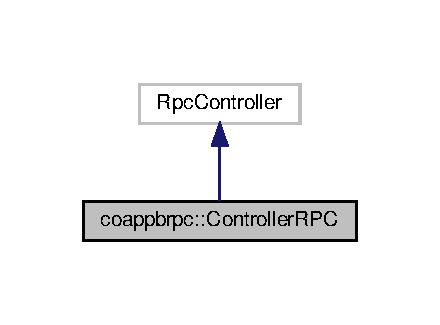
\includegraphics[width=211pt]{classcoappbrpc_1_1ControllerRPC__inherit__graph}
\end{center}
\end{figure}


Collaboration diagram for coappbrpc\+:\+:Controller\+R\+PC\+:\nopagebreak
\begin{figure}[H]
\begin{center}
\leavevmode
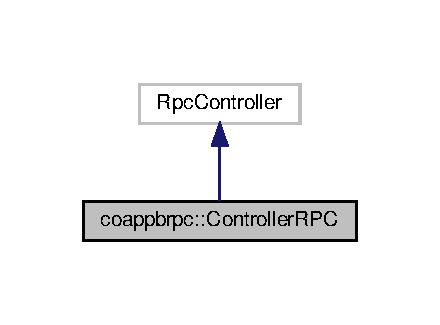
\includegraphics[width=211pt]{classcoappbrpc_1_1ControllerRPC__coll__graph}
\end{center}
\end{figure}
\subsection*{Public Member Functions}
\begin{DoxyCompactItemize}
\item 
\mbox{\Hypertarget{classcoappbrpc_1_1ControllerRPC_aac8d7a0e52a017d60a411a462bad6d91}\label{classcoappbrpc_1_1ControllerRPC_aac8d7a0e52a017d60a411a462bad6d91}} 
void \hyperlink{classcoappbrpc_1_1ControllerRPC_aac8d7a0e52a017d60a411a462bad6d91}{Reset} ()
\begin{DoxyCompactList}\small\item\em Resets m\+\_\+failed flag to false. \end{DoxyCompactList}\item 
\mbox{\Hypertarget{classcoappbrpc_1_1ControllerRPC_a20a3b119687bea2ac836db07a3b04287}\label{classcoappbrpc_1_1ControllerRPC_a20a3b119687bea2ac836db07a3b04287}} 
bool \hyperlink{classcoappbrpc_1_1ControllerRPC_a20a3b119687bea2ac836db07a3b04287}{Failed} () const
\begin{DoxyCompactList}\small\item\em getter function that returns m\+\_\+failed flag \end{DoxyCompactList}\item 
\mbox{\Hypertarget{classcoappbrpc_1_1ControllerRPC_a96035415234221d2972a3f2f790275ce}\label{classcoappbrpc_1_1ControllerRPC_a96035415234221d2972a3f2f790275ce}} 
string \hyperlink{classcoappbrpc_1_1ControllerRPC_a96035415234221d2972a3f2f790275ce}{Error\+Text} () const
\begin{DoxyCompactList}\small\item\em Getter function that returns message stored in m\+\_\+message. \end{DoxyCompactList}\item 
void \hyperlink{classcoappbrpc_1_1ControllerRPC_a3d91a6d0ba16232c531c3313e4412212}{Set\+Failed} (const string \&reason)
\begin{DoxyCompactList}\small\item\em Setter function which sets m\+\_\+failed to true when R\+PC fails and set m\+\_\+message to the reason of failure sent as parameter. \end{DoxyCompactList}\item 
void \hyperlink{classcoappbrpc_1_1ControllerRPC_a480586532b344e3ca8da2d2519ba593f}{append\+Failed} (const string \&reason)
\begin{DoxyCompactList}\small\item\em Function that appends multiple reasons for failure. \end{DoxyCompactList}\item 
\mbox{\Hypertarget{classcoappbrpc_1_1ControllerRPC_aab955bb22c799e5d544b3083fe64c7d7}\label{classcoappbrpc_1_1ControllerRPC_aab955bb22c799e5d544b3083fe64c7d7}} 
Error \hyperlink{classcoappbrpc_1_1ControllerRPC_aab955bb22c799e5d544b3083fe64c7d7}{error\+Obj} (void) const
\begin{DoxyCompactList}\small\item\em gets the Error object \end{DoxyCompactList}\item 
\mbox{\Hypertarget{classcoappbrpc_1_1ControllerRPC_a48a78ccc3c70a2135c78d612154e077c}\label{classcoappbrpc_1_1ControllerRPC_a48a78ccc3c70a2135c78d612154e077c}} 
void {\bfseries Start\+Cancel} ()
\item 
\mbox{\Hypertarget{classcoappbrpc_1_1ControllerRPC_ab6458ec248edf24fcc83b12a2573e13f}\label{classcoappbrpc_1_1ControllerRPC_ab6458ec248edf24fcc83b12a2573e13f}} 
bool {\bfseries Is\+Canceled} () const
\item 
\mbox{\Hypertarget{classcoappbrpc_1_1ControllerRPC_abc9385d7476171035cffb779c7966f89}\label{classcoappbrpc_1_1ControllerRPC_abc9385d7476171035cffb779c7966f89}} 
void {\bfseries Notify\+On\+Cancel} (Closure $\ast$callback)
\end{DoxyCompactItemize}


\subsection{Detailed Description}
This class inherits properties from google protobuf Rpc\+Controller, it has methods for resetting, setting failed, get error object if there is any error in the R\+PC. 

\subsection{Member Function Documentation}
\mbox{\Hypertarget{classcoappbrpc_1_1ControllerRPC_a480586532b344e3ca8da2d2519ba593f}\label{classcoappbrpc_1_1ControllerRPC_a480586532b344e3ca8da2d2519ba593f}} 
\index{coappbrpc\+::\+Controller\+R\+PC@{coappbrpc\+::\+Controller\+R\+PC}!append\+Failed@{append\+Failed}}
\index{append\+Failed@{append\+Failed}!coappbrpc\+::\+Controller\+R\+PC@{coappbrpc\+::\+Controller\+R\+PC}}
\subsubsection{\texorpdfstring{append\+Failed()}{appendFailed()}}
{\footnotesize\ttfamily void coappbrpc\+::\+Controller\+R\+P\+C\+::append\+Failed (\begin{DoxyParamCaption}\item[{const string \&}]{reason }\end{DoxyParamCaption})\hspace{0.3cm}{\ttfamily [inline]}}



Function that appends multiple reasons for failure. 


\begin{DoxyParams}{Parameters}
{\em reason} & string value that has explanation for failure \\
\hline
\end{DoxyParams}
\mbox{\Hypertarget{classcoappbrpc_1_1ControllerRPC_a3d91a6d0ba16232c531c3313e4412212}\label{classcoappbrpc_1_1ControllerRPC_a3d91a6d0ba16232c531c3313e4412212}} 
\index{coappbrpc\+::\+Controller\+R\+PC@{coappbrpc\+::\+Controller\+R\+PC}!Set\+Failed@{Set\+Failed}}
\index{Set\+Failed@{Set\+Failed}!coappbrpc\+::\+Controller\+R\+PC@{coappbrpc\+::\+Controller\+R\+PC}}
\subsubsection{\texorpdfstring{Set\+Failed()}{SetFailed()}}
{\footnotesize\ttfamily void coappbrpc\+::\+Controller\+R\+P\+C\+::\+Set\+Failed (\begin{DoxyParamCaption}\item[{const string \&}]{reason }\end{DoxyParamCaption})\hspace{0.3cm}{\ttfamily [inline]}}



Setter function which sets m\+\_\+failed to true when R\+PC fails and set m\+\_\+message to the reason of failure sent as parameter. 


\begin{DoxyParams}{Parameters}
{\em reason} & string value that has explanation for failure \\
\hline
\end{DoxyParams}


The documentation for this class was generated from the following file\+:\begin{DoxyCompactItemize}
\item 
include/\hyperlink{ControllerRPC_8h}{Controller\+R\+P\+C.\+h}\end{DoxyCompactItemize}

\hypertarget{classcoappbrpc_1_1Error}{}\section{coappbrpc\+:\+:Error Class Reference}
\label{classcoappbrpc_1_1Error}\index{coappbrpc\+::\+Error@{coappbrpc\+::\+Error}}


Inheritance diagram for coappbrpc\+:\+:Error\+:\nopagebreak
\begin{figure}[H]
\begin{center}
\leavevmode
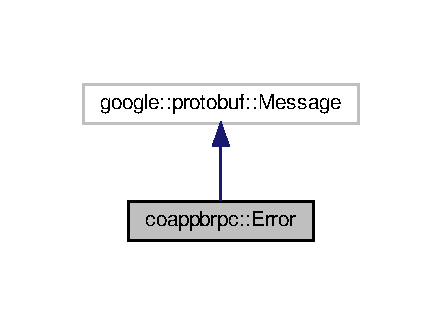
\includegraphics[width=212pt]{classcoappbrpc_1_1Error__inherit__graph}
\end{center}
\end{figure}


Collaboration diagram for coappbrpc\+:\+:Error\+:\nopagebreak
\begin{figure}[H]
\begin{center}
\leavevmode
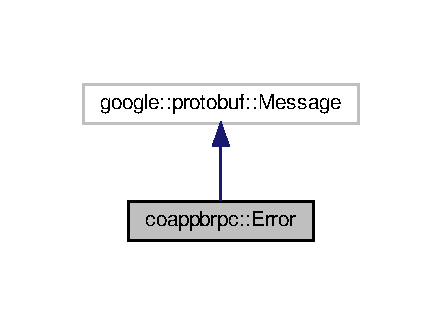
\includegraphics[width=212pt]{classcoappbrpc_1_1Error__coll__graph}
\end{center}
\end{figure}
\subsection*{Classes}
\begin{DoxyCompactItemize}
\item 
class \hyperlink{classcoappbrpc_1_1Error_1_1HasBitSetters}{Has\+Bit\+Setters}
\end{DoxyCompactItemize}
\subsection*{Public Member Functions}
\begin{DoxyCompactItemize}
\item 
\mbox{\Hypertarget{classcoappbrpc_1_1Error_a1a325665c85fc96f082a311cb3e3fc23}\label{classcoappbrpc_1_1Error_a1a325665c85fc96f082a311cb3e3fc23}} 
{\bfseries Error} (const \hyperlink{classcoappbrpc_1_1Error}{Error} \&from)
\item 
\mbox{\Hypertarget{classcoappbrpc_1_1Error_a06adcbeeca663447f9cf0387740f0744}\label{classcoappbrpc_1_1Error_a06adcbeeca663447f9cf0387740f0744}} 
\hyperlink{classcoappbrpc_1_1Error}{Error} \& {\bfseries operator=} (const \hyperlink{classcoappbrpc_1_1Error}{Error} \&from)
\item 
\mbox{\Hypertarget{classcoappbrpc_1_1Error_a0e09aab9715bdfa1c467f9ca7c4ed75a}\label{classcoappbrpc_1_1Error_a0e09aab9715bdfa1c467f9ca7c4ed75a}} 
void {\bfseries Swap} (\hyperlink{classcoappbrpc_1_1Error}{Error} $\ast$other)
\item 
\mbox{\Hypertarget{classcoappbrpc_1_1Error_ae52bf2329532524ec95a3e60225a62a2}\label{classcoappbrpc_1_1Error_ae52bf2329532524ec95a3e60225a62a2}} 
\hyperlink{classcoappbrpc_1_1Error}{Error} $\ast$ {\bfseries New} () const final
\item 
\mbox{\Hypertarget{classcoappbrpc_1_1Error_ac4bce964cb8730485d628a206af6d117}\label{classcoappbrpc_1_1Error_ac4bce964cb8730485d628a206af6d117}} 
\hyperlink{classcoappbrpc_1_1Error}{Error} $\ast$ {\bfseries New} (\+::google\+::protobuf\+::\+Arena $\ast$arena) const final
\item 
\mbox{\Hypertarget{classcoappbrpc_1_1Error_abf9ba3b9723a2d981aaf83d22ec8757a}\label{classcoappbrpc_1_1Error_abf9ba3b9723a2d981aaf83d22ec8757a}} 
void {\bfseries Copy\+From} (const \+::google\+::protobuf\+::\+Message \&from) final
\item 
\mbox{\Hypertarget{classcoappbrpc_1_1Error_ab853399916ca41d8eaa2aab0535533d0}\label{classcoappbrpc_1_1Error_ab853399916ca41d8eaa2aab0535533d0}} 
void {\bfseries Merge\+From} (const \+::google\+::protobuf\+::\+Message \&from) final
\item 
\mbox{\Hypertarget{classcoappbrpc_1_1Error_a52ca8b242a78f111be7735895160a1a3}\label{classcoappbrpc_1_1Error_a52ca8b242a78f111be7735895160a1a3}} 
void {\bfseries Copy\+From} (const \hyperlink{classcoappbrpc_1_1Error}{Error} \&from)
\item 
\mbox{\Hypertarget{classcoappbrpc_1_1Error_a9b8eca3a850aa4c53c8b46203c2dbffd}\label{classcoappbrpc_1_1Error_a9b8eca3a850aa4c53c8b46203c2dbffd}} 
void {\bfseries Merge\+From} (const \hyperlink{classcoappbrpc_1_1Error}{Error} \&from)
\item 
\mbox{\Hypertarget{classcoappbrpc_1_1Error_ad9e04e9f321d36f7f4fd97847cd228ce}\label{classcoappbrpc_1_1Error_ad9e04e9f321d36f7f4fd97847cd228ce}} 
void {\bfseries Clear} () final
\item 
\mbox{\Hypertarget{classcoappbrpc_1_1Error_ad9724721599eacc6eede185afac48793}\label{classcoappbrpc_1_1Error_ad9724721599eacc6eede185afac48793}} 
bool {\bfseries Is\+Initialized} () const final
\item 
\mbox{\Hypertarget{classcoappbrpc_1_1Error_aa858f0fd915c5692b4de0b551cb93b81}\label{classcoappbrpc_1_1Error_aa858f0fd915c5692b4de0b551cb93b81}} 
size\+\_\+t {\bfseries Byte\+Size\+Long} () const final
\item 
\mbox{\Hypertarget{classcoappbrpc_1_1Error_a615a3c932e6c7c1756cd1e53438cb119}\label{classcoappbrpc_1_1Error_a615a3c932e6c7c1756cd1e53438cb119}} 
bool {\bfseries Merge\+Partial\+From\+Coded\+Stream} (\+::google\+::protobuf\+::io\+::\+Coded\+Input\+Stream $\ast$input) final
\item 
\mbox{\Hypertarget{classcoappbrpc_1_1Error_a5cda1b9ed16feec0777bcbcf76f89c1e}\label{classcoappbrpc_1_1Error_a5cda1b9ed16feec0777bcbcf76f89c1e}} 
void {\bfseries Serialize\+With\+Cached\+Sizes} (\+::google\+::protobuf\+::io\+::\+Coded\+Output\+Stream $\ast$output) const final
\item 
\mbox{\Hypertarget{classcoappbrpc_1_1Error_a30aa6e3b7dbd72eabb6e1d962de68e8d}\label{classcoappbrpc_1_1Error_a30aa6e3b7dbd72eabb6e1d962de68e8d}} 
\+::google\+::protobuf\+::uint8 $\ast$ {\bfseries Internal\+Serialize\+With\+Cached\+Sizes\+To\+Array} (bool deterministic, \+::google\+::protobuf\+::uint8 $\ast$target) const final
\item 
\mbox{\Hypertarget{classcoappbrpc_1_1Error_a9b79b7d43fbbbb4f2e9172a1f898aeb4}\label{classcoappbrpc_1_1Error_a9b79b7d43fbbbb4f2e9172a1f898aeb4}} 
int {\bfseries Get\+Cached\+Size} () const final
\item 
\mbox{\Hypertarget{classcoappbrpc_1_1Error_a8803f21e0ec88ebc884b39923cfd3c7f}\label{classcoappbrpc_1_1Error_a8803f21e0ec88ebc884b39923cfd3c7f}} 
\+::google\+::protobuf\+::\+Metadata {\bfseries Get\+Metadata} () const final
\item 
\mbox{\Hypertarget{classcoappbrpc_1_1Error_a577934032656de1fa052835cad23626a}\label{classcoappbrpc_1_1Error_a577934032656de1fa052835cad23626a}} 
void {\bfseries clear\+\_\+message} ()
\item 
\mbox{\Hypertarget{classcoappbrpc_1_1Error_a9dc400abcdf851cec58bc02ebd2392cc}\label{classcoappbrpc_1_1Error_a9dc400abcdf851cec58bc02ebd2392cc}} 
const \+::std\+::string \& {\bfseries message} () const
\item 
\mbox{\Hypertarget{classcoappbrpc_1_1Error_a11354fca41ecfb10b1ae201c6232c8fd}\label{classcoappbrpc_1_1Error_a11354fca41ecfb10b1ae201c6232c8fd}} 
void {\bfseries set\+\_\+message} (const \+::std\+::string \&value)
\item 
\mbox{\Hypertarget{classcoappbrpc_1_1Error_ac7f5e9392eb8c448e87f23903c19c8aa}\label{classcoappbrpc_1_1Error_ac7f5e9392eb8c448e87f23903c19c8aa}} 
void {\bfseries set\+\_\+message} (const char $\ast$value)
\item 
\mbox{\Hypertarget{classcoappbrpc_1_1Error_a62ff01b3ac63dab5cb5b0f9c6973a5de}\label{classcoappbrpc_1_1Error_a62ff01b3ac63dab5cb5b0f9c6973a5de}} 
void {\bfseries set\+\_\+message} (const char $\ast$value, size\+\_\+t size)
\item 
\mbox{\Hypertarget{classcoappbrpc_1_1Error_a8b7ad03301f0e7ac9651f01144dbf82a}\label{classcoappbrpc_1_1Error_a8b7ad03301f0e7ac9651f01144dbf82a}} 
\+::std\+::string $\ast$ {\bfseries mutable\+\_\+message} ()
\item 
\mbox{\Hypertarget{classcoappbrpc_1_1Error_ab69f3ef2b76905f9843e9871c11a2d90}\label{classcoappbrpc_1_1Error_ab69f3ef2b76905f9843e9871c11a2d90}} 
\+::std\+::string $\ast$ {\bfseries release\+\_\+message} ()
\item 
\mbox{\Hypertarget{classcoappbrpc_1_1Error_aa481822f68e60ecd862635c6f2e3e397}\label{classcoappbrpc_1_1Error_aa481822f68e60ecd862635c6f2e3e397}} 
void {\bfseries set\+\_\+allocated\+\_\+message} (\+::std\+::string $\ast$message)
\item 
\mbox{\Hypertarget{classcoappbrpc_1_1Error_a223825c785dffa0c6184dba20c474a86}\label{classcoappbrpc_1_1Error_a223825c785dffa0c6184dba20c474a86}} 
void {\bfseries clear\+\_\+data} ()
\item 
\mbox{\Hypertarget{classcoappbrpc_1_1Error_af9cfa2e6266aeb1294ffef65da39da96}\label{classcoappbrpc_1_1Error_af9cfa2e6266aeb1294ffef65da39da96}} 
const \+::std\+::string \& {\bfseries data} () const
\item 
\mbox{\Hypertarget{classcoappbrpc_1_1Error_a1e65c8c348e8852ef6846621b317f22a}\label{classcoappbrpc_1_1Error_a1e65c8c348e8852ef6846621b317f22a}} 
void {\bfseries set\+\_\+data} (const \+::std\+::string \&value)
\item 
\mbox{\Hypertarget{classcoappbrpc_1_1Error_a71c4fff56dc64991d4b3aecf24778ad2}\label{classcoappbrpc_1_1Error_a71c4fff56dc64991d4b3aecf24778ad2}} 
void {\bfseries set\+\_\+data} (const char $\ast$value)
\item 
\mbox{\Hypertarget{classcoappbrpc_1_1Error_ab6fce8187d7f8b32aa627c394ff21ce1}\label{classcoappbrpc_1_1Error_ab6fce8187d7f8b32aa627c394ff21ce1}} 
void {\bfseries set\+\_\+data} (const void $\ast$value, size\+\_\+t size)
\item 
\mbox{\Hypertarget{classcoappbrpc_1_1Error_a43f80373d6775e1863b355c0bd80ac18}\label{classcoappbrpc_1_1Error_a43f80373d6775e1863b355c0bd80ac18}} 
\+::std\+::string $\ast$ {\bfseries mutable\+\_\+data} ()
\item 
\mbox{\Hypertarget{classcoappbrpc_1_1Error_ae54fc2d7f0a102d5b7a3b55a61bd96a1}\label{classcoappbrpc_1_1Error_ae54fc2d7f0a102d5b7a3b55a61bd96a1}} 
\+::std\+::string $\ast$ {\bfseries release\+\_\+data} ()
\item 
\mbox{\Hypertarget{classcoappbrpc_1_1Error_aeae3dd27dabf24258646616365846a22}\label{classcoappbrpc_1_1Error_aeae3dd27dabf24258646616365846a22}} 
void {\bfseries set\+\_\+allocated\+\_\+data} (\+::std\+::string $\ast$data)
\end{DoxyCompactItemize}
\subsection*{Static Public Member Functions}
\begin{DoxyCompactItemize}
\item 
\mbox{\Hypertarget{classcoappbrpc_1_1Error_a835816ae390a4823c3cda44d0eea4ac2}\label{classcoappbrpc_1_1Error_a835816ae390a4823c3cda44d0eea4ac2}} 
static const \+::google\+::protobuf\+::\+Descriptor $\ast$ {\bfseries descriptor} ()
\item 
\mbox{\Hypertarget{classcoappbrpc_1_1Error_ae4e0a093db086c07b372c9fed1b76b18}\label{classcoappbrpc_1_1Error_ae4e0a093db086c07b372c9fed1b76b18}} 
static const \hyperlink{classcoappbrpc_1_1Error}{Error} \& {\bfseries default\+\_\+instance} ()
\item 
\mbox{\Hypertarget{classcoappbrpc_1_1Error_a9ef5aed94b431be32ae561055e86da91}\label{classcoappbrpc_1_1Error_a9ef5aed94b431be32ae561055e86da91}} 
static void {\bfseries Init\+As\+Default\+Instance} ()
\item 
\mbox{\Hypertarget{classcoappbrpc_1_1Error_a054f12c7ba5aa48ac9e29c89eadfa00f}\label{classcoappbrpc_1_1Error_a054f12c7ba5aa48ac9e29c89eadfa00f}} 
static const \hyperlink{classcoappbrpc_1_1Error}{Error} $\ast$ {\bfseries internal\+\_\+default\+\_\+instance} ()
\end{DoxyCompactItemize}
\subsection*{Static Public Attributes}
\begin{DoxyCompactItemize}
\item 
static constexpr int {\bfseries k\+Index\+In\+File\+Messages}
\item 
\mbox{\Hypertarget{classcoappbrpc_1_1Error_ac3b04639b8436127975805d710defdaa}\label{classcoappbrpc_1_1Error_ac3b04639b8436127975805d710defdaa}} 
static const int {\bfseries k\+Message\+Field\+Number} = 1
\item 
\mbox{\Hypertarget{classcoappbrpc_1_1Error_afdf01e84439d824f3f8276b0fc18189a}\label{classcoappbrpc_1_1Error_afdf01e84439d824f3f8276b0fc18189a}} 
static const int {\bfseries k\+Data\+Field\+Number} = 2
\end{DoxyCompactItemize}
\subsection*{Friends}
\begin{DoxyCompactItemize}
\item 
\mbox{\Hypertarget{classcoappbrpc_1_1Error_a65c087bf06ded9c9be363691f7b7bafa}\label{classcoappbrpc_1_1Error_a65c087bf06ded9c9be363691f7b7bafa}} 
struct {\bfseries \+::\+Table\+Struct\+\_\+\+Msg\+Schema\+\_\+2eproto}
\item 
\mbox{\Hypertarget{classcoappbrpc_1_1Error_a8a56a72c6855aff317cf18b3c5f2fa5d}\label{classcoappbrpc_1_1Error_a8a56a72c6855aff317cf18b3c5f2fa5d}} 
void {\bfseries swap} (\hyperlink{classcoappbrpc_1_1Error}{Error} \&a, \hyperlink{classcoappbrpc_1_1Error}{Error} \&b)
\end{DoxyCompactItemize}


\subsection{Member Data Documentation}
\mbox{\Hypertarget{classcoappbrpc_1_1Error_a92d90802862d90205267fb130aa544b9}\label{classcoappbrpc_1_1Error_a92d90802862d90205267fb130aa544b9}} 
\index{coappbrpc\+::\+Error@{coappbrpc\+::\+Error}!k\+Index\+In\+File\+Messages@{k\+Index\+In\+File\+Messages}}
\index{k\+Index\+In\+File\+Messages@{k\+Index\+In\+File\+Messages}!coappbrpc\+::\+Error@{coappbrpc\+::\+Error}}
\subsubsection{\texorpdfstring{k\+Index\+In\+File\+Messages}{kIndexInFileMessages}}
{\footnotesize\ttfamily constexpr int coappbrpc\+::\+Error\+::k\+Index\+In\+File\+Messages\hspace{0.3cm}{\ttfamily [static]}}

{\bfseries Initial value\+:}
\begin{DoxyCode}
=
    1
\end{DoxyCode}


The documentation for this class was generated from the following files\+:\begin{DoxyCompactItemize}
\item 
build/proto/Msg\+Schema.\+pb.\+h\item 
build/proto/Msg\+Schema.\+pb.\+cc\end{DoxyCompactItemize}

\hypertarget{classcoappbrpc_1_1ErrorDefaultTypeInternal}{}\section{coappbrpc\+:\+:Error\+Default\+Type\+Internal Class Reference}
\label{classcoappbrpc_1_1ErrorDefaultTypeInternal}\index{coappbrpc\+::\+Error\+Default\+Type\+Internal@{coappbrpc\+::\+Error\+Default\+Type\+Internal}}
\subsection*{Public Attributes}
\begin{DoxyCompactItemize}
\item 
\mbox{\Hypertarget{classcoappbrpc_1_1ErrorDefaultTypeInternal_ade1a1ad28e83164588942a5e28bf23c5}\label{classcoappbrpc_1_1ErrorDefaultTypeInternal_ade1a1ad28e83164588942a5e28bf23c5}} 
\+::google\+::protobuf\+::internal\+::\+Explicitly\+Constructed$<$ \hyperlink{classcoappbrpc_1_1Error}{Error} $>$ {\bfseries \+\_\+instance}
\end{DoxyCompactItemize}


The documentation for this class was generated from the following file\+:\begin{DoxyCompactItemize}
\item 
build/proto/Msg\+Schema.\+pb.\+cc\end{DoxyCompactItemize}

\hypertarget{classGreeterClient}{}\section{Greeter\+Client Class Reference}
\label{classGreeterClient}\index{Greeter\+Client@{Greeter\+Client}}
\subsection*{Public Member Functions}
\begin{DoxyCompactItemize}
\item 
\mbox{\Hypertarget{classGreeterClient_a673a567cdce22eeed0afaf48bf808fa8}\label{classGreeterClient_a673a567cdce22eeed0afaf48bf808fa8}} 
string {\bfseries Say\+Hello} (const std\+::string \&user)
\end{DoxyCompactItemize}


The documentation for this class was generated from the following file\+:\begin{DoxyCompactItemize}
\item 
example/helloworld/client.\+cpp\end{DoxyCompactItemize}

\hypertarget{classcoappbrpc_1_1api_1_1GreeterServiceImpl}{}\section{coappbrpc\+:\+:api\+:\+:Greeter\+Service\+Impl Class Reference}
\label{classcoappbrpc_1_1api_1_1GreeterServiceImpl}\index{coappbrpc\+::api\+::\+Greeter\+Service\+Impl@{coappbrpc\+::api\+::\+Greeter\+Service\+Impl}}


Inheritance diagram for coappbrpc\+:\+:api\+:\+:Greeter\+Service\+Impl\+:
\nopagebreak
\begin{figure}[H]
\begin{center}
\leavevmode
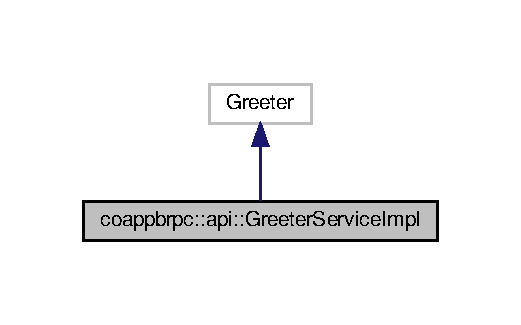
\includegraphics[width=250pt]{classcoappbrpc_1_1api_1_1GreeterServiceImpl__inherit__graph}
\end{center}
\end{figure}


Collaboration diagram for coappbrpc\+:\+:api\+:\+:Greeter\+Service\+Impl\+:
\nopagebreak
\begin{figure}[H]
\begin{center}
\leavevmode
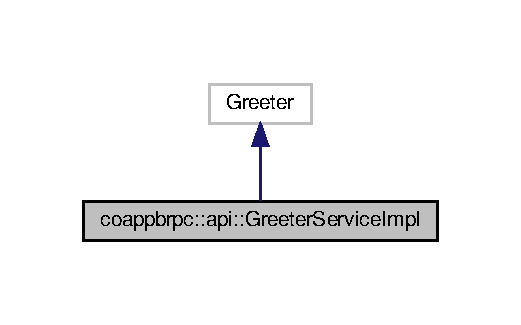
\includegraphics[width=250pt]{classcoappbrpc_1_1api_1_1GreeterServiceImpl__coll__graph}
\end{center}
\end{figure}
\subsection*{Public Member Functions}
\begin{DoxyCompactItemize}
\item 
\mbox{\Hypertarget{classcoappbrpc_1_1api_1_1GreeterServiceImpl_a009b97643d9728170104e367b8f40167}\label{classcoappbrpc_1_1api_1_1GreeterServiceImpl_a009b97643d9728170104e367b8f40167}} 
virtual void {\bfseries Say\+Hello} (Rpc\+Controller $\ast$controller, const Hello\+Request $\ast$request, Hello\+Reply $\ast$reply, Closure $\ast$done)
\end{DoxyCompactItemize}


The documentation for this class was generated from the following file\+:\begin{DoxyCompactItemize}
\item 
example/helloworld/server.\+cpp\end{DoxyCompactItemize}

\hypertarget{classcoappbrpc_1_1Request_1_1HasBitSetters}{}\section{coappbrpc\+:\+:Request\+:\+:Has\+Bit\+Setters Class Reference}
\label{classcoappbrpc_1_1Request_1_1HasBitSetters}\index{coappbrpc\+::\+Request\+::\+Has\+Bit\+Setters@{coappbrpc\+::\+Request\+::\+Has\+Bit\+Setters}}


The documentation for this class was generated from the following file\+:\begin{DoxyCompactItemize}
\item 
build/proto/Msg\+Schema.\+pb.\+cc\end{DoxyCompactItemize}

\hypertarget{classcoappbrpc_1_1Error_1_1HasBitSetters}{}\section{coappbrpc\+:\+:Error\+:\+:Has\+Bit\+Setters Class Reference}
\label{classcoappbrpc_1_1Error_1_1HasBitSetters}\index{coappbrpc\+::\+Error\+::\+Has\+Bit\+Setters@{coappbrpc\+::\+Error\+::\+Has\+Bit\+Setters}}


The documentation for this class was generated from the following file\+:\begin{DoxyCompactItemize}
\item 
build/proto/Msg\+Schema.\+pb.\+cc\end{DoxyCompactItemize}

\hypertarget{classcoappbrpc_1_1Response_1_1HasBitSetters}{}\section{coappbrpc\+:\+:Response\+:\+:Has\+Bit\+Setters Class Reference}
\label{classcoappbrpc_1_1Response_1_1HasBitSetters}\index{coappbrpc\+::\+Response\+::\+Has\+Bit\+Setters@{coappbrpc\+::\+Response\+::\+Has\+Bit\+Setters}}
\subsection*{Static Public Member Functions}
\begin{DoxyCompactItemize}
\item 
\mbox{\Hypertarget{classcoappbrpc_1_1Response_1_1HasBitSetters_afe7b2e5cad486fab4e12b8f92d20a5af}\label{classcoappbrpc_1_1Response_1_1HasBitSetters_afe7b2e5cad486fab4e12b8f92d20a5af}} 
static const \+::\hyperlink{classcoappbrpc_1_1Error}{coappbrpc\+::\+Error} \& {\bfseries error} (const \hyperlink{classcoappbrpc_1_1Response}{Response} $\ast$msg)
\end{DoxyCompactItemize}


The documentation for this class was generated from the following file\+:\begin{DoxyCompactItemize}
\item 
build/proto/Msg\+Schema.\+pb.\+cc\end{DoxyCompactItemize}

\hypertarget{classPingClient}{}\section{Ping\+Client Class Reference}
\label{classPingClient}\index{Ping\+Client@{Ping\+Client}}
\subsection*{Public Member Functions}
\begin{DoxyCompactItemize}
\item 
\mbox{\Hypertarget{classPingClient_a888873d874335defed11102c757e0612}\label{classPingClient_a888873d874335defed11102c757e0612}} 
string {\bfseries ping} (const string \&msg)
\end{DoxyCompactItemize}


The documentation for this class was generated from the following file\+:\begin{DoxyCompactItemize}
\item 
example/ping/client.\+cpp\end{DoxyCompactItemize}

\hypertarget{classcoappbrpc_1_1api_1_1PingServiceImpl}{}\section{coappbrpc\+:\+:api\+:\+:Ping\+Service\+Impl Class Reference}
\label{classcoappbrpc_1_1api_1_1PingServiceImpl}\index{coappbrpc\+::api\+::\+Ping\+Service\+Impl@{coappbrpc\+::api\+::\+Ping\+Service\+Impl}}


Inheritance diagram for coappbrpc\+:\+:api\+:\+:Ping\+Service\+Impl\+:
\nopagebreak
\begin{figure}[H]
\begin{center}
\leavevmode
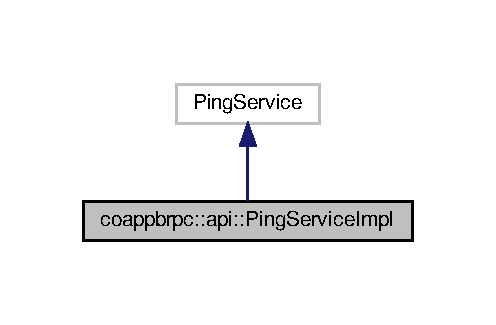
\includegraphics[width=238pt]{classcoappbrpc_1_1api_1_1PingServiceImpl__inherit__graph}
\end{center}
\end{figure}


Collaboration diagram for coappbrpc\+:\+:api\+:\+:Ping\+Service\+Impl\+:
\nopagebreak
\begin{figure}[H]
\begin{center}
\leavevmode
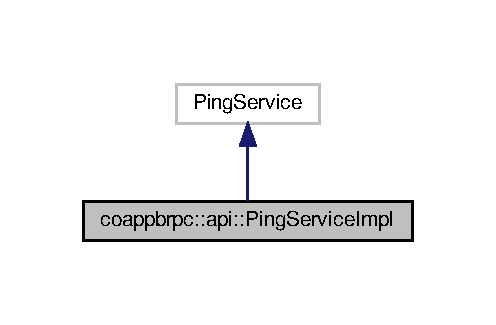
\includegraphics[width=238pt]{classcoappbrpc_1_1api_1_1PingServiceImpl__coll__graph}
\end{center}
\end{figure}
\subsection*{Public Member Functions}
\begin{DoxyCompactItemize}
\item 
\mbox{\Hypertarget{classcoappbrpc_1_1api_1_1PingServiceImpl_ad0fdead8e69607ba9114b277fe96844b}\label{classcoappbrpc_1_1api_1_1PingServiceImpl_ad0fdead8e69607ba9114b277fe96844b}} 
virtual void {\bfseries Ping} (Rpc\+Controller $\ast$controller, const Ping\+Request $\ast$request, Ping\+Response $\ast$response, Closure $\ast$done)
\end{DoxyCompactItemize}


The documentation for this class was generated from the following file\+:\begin{DoxyCompactItemize}
\item 
example/ping/server.\+cpp\end{DoxyCompactItemize}

\hypertarget{classcoappbrpc_1_1Request}{}\section{coappbrpc\+:\+:Request Class Reference}
\label{classcoappbrpc_1_1Request}\index{coappbrpc\+::\+Request@{coappbrpc\+::\+Request}}


Inheritance diagram for coappbrpc\+:\+:Request\+:
% FIG 0


Collaboration diagram for coappbrpc\+:\+:Request\+:
% FIG 1
\subsection*{Classes}
\begin{DoxyCompactItemize}
\item 
class \hyperlink{classcoappbrpc_1_1Request_1_1HasBitSetters}{Has\+Bit\+Setters}
\end{DoxyCompactItemize}
\subsection*{Public Member Functions}
\begin{DoxyCompactItemize}
\item 
\mbox{\Hypertarget{classcoappbrpc_1_1Request_a47a39167c3ce45e3c3fd7e02b1fc543d}\label{classcoappbrpc_1_1Request_a47a39167c3ce45e3c3fd7e02b1fc543d}} 
{\bfseries Request} (const \hyperlink{classcoappbrpc_1_1Request}{Request} \&from)
\item 
\mbox{\Hypertarget{classcoappbrpc_1_1Request_a16ffbdf9dda710d5118fa74bac52d61a}\label{classcoappbrpc_1_1Request_a16ffbdf9dda710d5118fa74bac52d61a}} 
\hyperlink{classcoappbrpc_1_1Request}{Request} \& {\bfseries operator=} (const \hyperlink{classcoappbrpc_1_1Request}{Request} \&from)
\item 
\mbox{\Hypertarget{classcoappbrpc_1_1Request_a98653b1ed247cbb328495fe00c8741b1}\label{classcoappbrpc_1_1Request_a98653b1ed247cbb328495fe00c8741b1}} 
void {\bfseries Swap} (\hyperlink{classcoappbrpc_1_1Request}{Request} $\ast$other)
\item 
\mbox{\Hypertarget{classcoappbrpc_1_1Request_aeff1989d6f4b25ae7923492201489f75}\label{classcoappbrpc_1_1Request_aeff1989d6f4b25ae7923492201489f75}} 
\hyperlink{classcoappbrpc_1_1Request}{Request} $\ast$ {\bfseries New} () const final
\item 
\mbox{\Hypertarget{classcoappbrpc_1_1Request_a9b3c97de3afd1435da415cf623ca5a49}\label{classcoappbrpc_1_1Request_a9b3c97de3afd1435da415cf623ca5a49}} 
\hyperlink{classcoappbrpc_1_1Request}{Request} $\ast$ {\bfseries New} (\+::google\+::protobuf\+::\+Arena $\ast$arena) const final
\item 
\mbox{\Hypertarget{classcoappbrpc_1_1Request_a4d2f9d18648487a08edb25e1f9a6a4c2}\label{classcoappbrpc_1_1Request_a4d2f9d18648487a08edb25e1f9a6a4c2}} 
void {\bfseries Copy\+From} (const \+::google\+::protobuf\+::\+Message \&from) final
\item 
\mbox{\Hypertarget{classcoappbrpc_1_1Request_a74dcbf992d27f7d18822e381dac3713c}\label{classcoappbrpc_1_1Request_a74dcbf992d27f7d18822e381dac3713c}} 
void {\bfseries Merge\+From} (const \+::google\+::protobuf\+::\+Message \&from) final
\item 
\mbox{\Hypertarget{classcoappbrpc_1_1Request_a4c74f0343c8b770aab1074a3571ba9ce}\label{classcoappbrpc_1_1Request_a4c74f0343c8b770aab1074a3571ba9ce}} 
void {\bfseries Copy\+From} (const \hyperlink{classcoappbrpc_1_1Request}{Request} \&from)
\item 
\mbox{\Hypertarget{classcoappbrpc_1_1Request_a745157bc69afe4509e157ca9835e2d9c}\label{classcoappbrpc_1_1Request_a745157bc69afe4509e157ca9835e2d9c}} 
void {\bfseries Merge\+From} (const \hyperlink{classcoappbrpc_1_1Request}{Request} \&from)
\item 
\mbox{\Hypertarget{classcoappbrpc_1_1Request_a3699329574cf56b9b684dcb984176910}\label{classcoappbrpc_1_1Request_a3699329574cf56b9b684dcb984176910}} 
void {\bfseries Clear} () final
\item 
\mbox{\Hypertarget{classcoappbrpc_1_1Request_a3b3733fa1bb216ecaa3013b506485bf3}\label{classcoappbrpc_1_1Request_a3b3733fa1bb216ecaa3013b506485bf3}} 
bool {\bfseries Is\+Initialized} () const final
\item 
\mbox{\Hypertarget{classcoappbrpc_1_1Request_af3933a049ac9a8bcae6efeccb6be6823}\label{classcoappbrpc_1_1Request_af3933a049ac9a8bcae6efeccb6be6823}} 
size\+\_\+t {\bfseries Byte\+Size\+Long} () const final
\item 
\mbox{\Hypertarget{classcoappbrpc_1_1Request_a590deeb6a5bf95ab9e0bdbff4d6ed92a}\label{classcoappbrpc_1_1Request_a590deeb6a5bf95ab9e0bdbff4d6ed92a}} 
bool {\bfseries Merge\+Partial\+From\+Coded\+Stream} (\+::google\+::protobuf\+::io\+::\+Coded\+Input\+Stream $\ast$input) final
\item 
\mbox{\Hypertarget{classcoappbrpc_1_1Request_a707fec97351a1cf2e2af40c4628579a4}\label{classcoappbrpc_1_1Request_a707fec97351a1cf2e2af40c4628579a4}} 
void {\bfseries Serialize\+With\+Cached\+Sizes} (\+::google\+::protobuf\+::io\+::\+Coded\+Output\+Stream $\ast$output) const final
\item 
\mbox{\Hypertarget{classcoappbrpc_1_1Request_abf99985c08c4b47e71275959b2a5a643}\label{classcoappbrpc_1_1Request_abf99985c08c4b47e71275959b2a5a643}} 
\+::google\+::protobuf\+::uint8 $\ast$ {\bfseries Internal\+Serialize\+With\+Cached\+Sizes\+To\+Array} (bool deterministic, \+::google\+::protobuf\+::uint8 $\ast$target) const final
\item 
\mbox{\Hypertarget{classcoappbrpc_1_1Request_a3e6421e0c870ce79d40ad896db78d0c7}\label{classcoappbrpc_1_1Request_a3e6421e0c870ce79d40ad896db78d0c7}} 
int {\bfseries Get\+Cached\+Size} () const final
\item 
\mbox{\Hypertarget{classcoappbrpc_1_1Request_a09b5a02b3a1a5b62d9cc02e5861cebe4}\label{classcoappbrpc_1_1Request_a09b5a02b3a1a5b62d9cc02e5861cebe4}} 
\+::google\+::protobuf\+::\+Metadata {\bfseries Get\+Metadata} () const final
\item 
\mbox{\Hypertarget{classcoappbrpc_1_1Request_a9ede440fd8f0d845e4fe8ce1deb5973f}\label{classcoappbrpc_1_1Request_a9ede440fd8f0d845e4fe8ce1deb5973f}} 
void {\bfseries clear\+\_\+version} ()
\item 
\mbox{\Hypertarget{classcoappbrpc_1_1Request_a35f5cd80696f6c7b56c4d4e24d1f344a}\label{classcoappbrpc_1_1Request_a35f5cd80696f6c7b56c4d4e24d1f344a}} 
const \+::std\+::string \& {\bfseries version} () const
\item 
\mbox{\Hypertarget{classcoappbrpc_1_1Request_a6563f82b332ac0714c61daa2ad010374}\label{classcoappbrpc_1_1Request_a6563f82b332ac0714c61daa2ad010374}} 
void {\bfseries set\+\_\+version} (const \+::std\+::string \&value)
\item 
\mbox{\Hypertarget{classcoappbrpc_1_1Request_ad431e4dc189a9e3ebe32b5d058727b69}\label{classcoappbrpc_1_1Request_ad431e4dc189a9e3ebe32b5d058727b69}} 
void {\bfseries set\+\_\+version} (const char $\ast$value)
\item 
\mbox{\Hypertarget{classcoappbrpc_1_1Request_a3111278b77ba1c4b5b1531df140124f2}\label{classcoappbrpc_1_1Request_a3111278b77ba1c4b5b1531df140124f2}} 
void {\bfseries set\+\_\+version} (const char $\ast$value, size\+\_\+t size)
\item 
\mbox{\Hypertarget{classcoappbrpc_1_1Request_ae9ec424b715eace57f2d6dc7d500f286}\label{classcoappbrpc_1_1Request_ae9ec424b715eace57f2d6dc7d500f286}} 
\+::std\+::string $\ast$ {\bfseries mutable\+\_\+version} ()
\item 
\mbox{\Hypertarget{classcoappbrpc_1_1Request_a06f0d58dc46d2fae775c5dfdc71458be}\label{classcoappbrpc_1_1Request_a06f0d58dc46d2fae775c5dfdc71458be}} 
\+::std\+::string $\ast$ {\bfseries release\+\_\+version} ()
\item 
\mbox{\Hypertarget{classcoappbrpc_1_1Request_a6b06bcc01a30ab256cf15dd18089eeab}\label{classcoappbrpc_1_1Request_a6b06bcc01a30ab256cf15dd18089eeab}} 
void {\bfseries set\+\_\+allocated\+\_\+version} (\+::std\+::string $\ast$version)
\item 
\mbox{\Hypertarget{classcoappbrpc_1_1Request_a0fc178adfb20c19e00eeaab82b80f53f}\label{classcoappbrpc_1_1Request_a0fc178adfb20c19e00eeaab82b80f53f}} 
void {\bfseries clear\+\_\+service} ()
\item 
\mbox{\Hypertarget{classcoappbrpc_1_1Request_a7ad2daa87ccc004815226d499e958413}\label{classcoappbrpc_1_1Request_a7ad2daa87ccc004815226d499e958413}} 
const \+::std\+::string \& {\bfseries service} () const
\item 
\mbox{\Hypertarget{classcoappbrpc_1_1Request_afeac2f99fef1585356a8f3ac97b0f75e}\label{classcoappbrpc_1_1Request_afeac2f99fef1585356a8f3ac97b0f75e}} 
void {\bfseries set\+\_\+service} (const \+::std\+::string \&value)
\item 
\mbox{\Hypertarget{classcoappbrpc_1_1Request_a36bacf2f08ded736916657c94b14fc60}\label{classcoappbrpc_1_1Request_a36bacf2f08ded736916657c94b14fc60}} 
void {\bfseries set\+\_\+service} (const char $\ast$value)
\item 
\mbox{\Hypertarget{classcoappbrpc_1_1Request_aa59b8a2db7fcf08849232a23d90260d0}\label{classcoappbrpc_1_1Request_aa59b8a2db7fcf08849232a23d90260d0}} 
void {\bfseries set\+\_\+service} (const char $\ast$value, size\+\_\+t size)
\item 
\mbox{\Hypertarget{classcoappbrpc_1_1Request_a9fb0e2a179f69ad34a07025789a000d5}\label{classcoappbrpc_1_1Request_a9fb0e2a179f69ad34a07025789a000d5}} 
\+::std\+::string $\ast$ {\bfseries mutable\+\_\+service} ()
\item 
\mbox{\Hypertarget{classcoappbrpc_1_1Request_ad24c1c227bf3b8bd1c2ee60c3617eb7c}\label{classcoappbrpc_1_1Request_ad24c1c227bf3b8bd1c2ee60c3617eb7c}} 
\+::std\+::string $\ast$ {\bfseries release\+\_\+service} ()
\item 
\mbox{\Hypertarget{classcoappbrpc_1_1Request_a59e8d08d63e9f91ea83cad31d73ae7e6}\label{classcoappbrpc_1_1Request_a59e8d08d63e9f91ea83cad31d73ae7e6}} 
void {\bfseries set\+\_\+allocated\+\_\+service} (\+::std\+::string $\ast$service)
\item 
\mbox{\Hypertarget{classcoappbrpc_1_1Request_a0bf017c8c04f9ba6c9008d56ea417e70}\label{classcoappbrpc_1_1Request_a0bf017c8c04f9ba6c9008d56ea417e70}} 
void {\bfseries clear\+\_\+method} ()
\item 
\mbox{\Hypertarget{classcoappbrpc_1_1Request_a0fd5b103c1ce2681040a80f88fdb8b37}\label{classcoappbrpc_1_1Request_a0fd5b103c1ce2681040a80f88fdb8b37}} 
const \+::std\+::string \& {\bfseries method} () const
\item 
\mbox{\Hypertarget{classcoappbrpc_1_1Request_abce4c7d94de659fe0b1078907fade489}\label{classcoappbrpc_1_1Request_abce4c7d94de659fe0b1078907fade489}} 
void {\bfseries set\+\_\+method} (const \+::std\+::string \&value)
\item 
\mbox{\Hypertarget{classcoappbrpc_1_1Request_a578f6f991711590b9c55e17581f8561c}\label{classcoappbrpc_1_1Request_a578f6f991711590b9c55e17581f8561c}} 
void {\bfseries set\+\_\+method} (const char $\ast$value)
\item 
\mbox{\Hypertarget{classcoappbrpc_1_1Request_abb7aa04c7773dedb82e60d5569f3aa78}\label{classcoappbrpc_1_1Request_abb7aa04c7773dedb82e60d5569f3aa78}} 
void {\bfseries set\+\_\+method} (const char $\ast$value, size\+\_\+t size)
\item 
\mbox{\Hypertarget{classcoappbrpc_1_1Request_a1145ab28351a4c3f8dd846ce17770730}\label{classcoappbrpc_1_1Request_a1145ab28351a4c3f8dd846ce17770730}} 
\+::std\+::string $\ast$ {\bfseries mutable\+\_\+method} ()
\item 
\mbox{\Hypertarget{classcoappbrpc_1_1Request_a2394d4827b0c92238294c38424590419}\label{classcoappbrpc_1_1Request_a2394d4827b0c92238294c38424590419}} 
\+::std\+::string $\ast$ {\bfseries release\+\_\+method} ()
\item 
\mbox{\Hypertarget{classcoappbrpc_1_1Request_abc69e31e8d9b71ad106e57386d14891d}\label{classcoappbrpc_1_1Request_abc69e31e8d9b71ad106e57386d14891d}} 
void {\bfseries set\+\_\+allocated\+\_\+method} (\+::std\+::string $\ast$method)
\item 
\mbox{\Hypertarget{classcoappbrpc_1_1Request_a80b1ab7b95c197b7d7c7ef01d478d5c9}\label{classcoappbrpc_1_1Request_a80b1ab7b95c197b7d7c7ef01d478d5c9}} 
void {\bfseries clear\+\_\+params} ()
\item 
\mbox{\Hypertarget{classcoappbrpc_1_1Request_a475de4a3d35e86c91adad2b824bbd52d}\label{classcoappbrpc_1_1Request_a475de4a3d35e86c91adad2b824bbd52d}} 
const \+::std\+::string \& {\bfseries params} () const
\item 
\mbox{\Hypertarget{classcoappbrpc_1_1Request_a738278b90cadfe2e5452ade21fd34691}\label{classcoappbrpc_1_1Request_a738278b90cadfe2e5452ade21fd34691}} 
void {\bfseries set\+\_\+params} (const \+::std\+::string \&value)
\item 
\mbox{\Hypertarget{classcoappbrpc_1_1Request_a37741785a7e7ea8498839962a575d319}\label{classcoappbrpc_1_1Request_a37741785a7e7ea8498839962a575d319}} 
void {\bfseries set\+\_\+params} (const char $\ast$value)
\item 
\mbox{\Hypertarget{classcoappbrpc_1_1Request_a9fcffc4c495208606973bc8b6683248d}\label{classcoappbrpc_1_1Request_a9fcffc4c495208606973bc8b6683248d}} 
void {\bfseries set\+\_\+params} (const void $\ast$value, size\+\_\+t size)
\item 
\mbox{\Hypertarget{classcoappbrpc_1_1Request_a42c21d76e979369b8df159a1b1b03573}\label{classcoappbrpc_1_1Request_a42c21d76e979369b8df159a1b1b03573}} 
\+::std\+::string $\ast$ {\bfseries mutable\+\_\+params} ()
\item 
\mbox{\Hypertarget{classcoappbrpc_1_1Request_a2aec9643c67b70935692a3648af508aa}\label{classcoappbrpc_1_1Request_a2aec9643c67b70935692a3648af508aa}} 
\+::std\+::string $\ast$ {\bfseries release\+\_\+params} ()
\item 
\mbox{\Hypertarget{classcoappbrpc_1_1Request_aa7f19fbcc325f288b0d70b3e3eb55829}\label{classcoappbrpc_1_1Request_aa7f19fbcc325f288b0d70b3e3eb55829}} 
void {\bfseries set\+\_\+allocated\+\_\+params} (\+::std\+::string $\ast$params)
\item 
\mbox{\Hypertarget{classcoappbrpc_1_1Request_a687f7932f9718823e114a934d5d4a41f}\label{classcoappbrpc_1_1Request_a687f7932f9718823e114a934d5d4a41f}} 
void {\bfseries clear\+\_\+id} ()
\item 
\mbox{\Hypertarget{classcoappbrpc_1_1Request_a48a39437866e9a8f9ee50759966cbc7e}\label{classcoappbrpc_1_1Request_a48a39437866e9a8f9ee50759966cbc7e}} 
\+::google\+::protobuf\+::int32 {\bfseries id} () const
\item 
\mbox{\Hypertarget{classcoappbrpc_1_1Request_a6d5f7f9cbd2757ff922ed6339055dc5b}\label{classcoappbrpc_1_1Request_a6d5f7f9cbd2757ff922ed6339055dc5b}} 
void {\bfseries set\+\_\+id} (\+::google\+::protobuf\+::int32 value)
\end{DoxyCompactItemize}
\subsection*{Static Public Member Functions}
\begin{DoxyCompactItemize}
\item 
\mbox{\Hypertarget{classcoappbrpc_1_1Request_acee20e2a177227b514ff52c82cc23cdf}\label{classcoappbrpc_1_1Request_acee20e2a177227b514ff52c82cc23cdf}} 
static const \+::google\+::protobuf\+::\+Descriptor $\ast$ {\bfseries descriptor} ()
\item 
\mbox{\Hypertarget{classcoappbrpc_1_1Request_a24d20d232627a8baaf01bb0ed9266c46}\label{classcoappbrpc_1_1Request_a24d20d232627a8baaf01bb0ed9266c46}} 
static const \hyperlink{classcoappbrpc_1_1Request}{Request} \& {\bfseries default\+\_\+instance} ()
\item 
\mbox{\Hypertarget{classcoappbrpc_1_1Request_aa650d4a3da3187eb70e13f0d7931bad6}\label{classcoappbrpc_1_1Request_aa650d4a3da3187eb70e13f0d7931bad6}} 
static void {\bfseries Init\+As\+Default\+Instance} ()
\item 
\mbox{\Hypertarget{classcoappbrpc_1_1Request_a6f72b785009d065f41981a2a7ad8f294}\label{classcoappbrpc_1_1Request_a6f72b785009d065f41981a2a7ad8f294}} 
static const \hyperlink{classcoappbrpc_1_1Request}{Request} $\ast$ {\bfseries internal\+\_\+default\+\_\+instance} ()
\end{DoxyCompactItemize}
\subsection*{Static Public Attributes}
\begin{DoxyCompactItemize}
\item 
static constexpr int {\bfseries k\+Index\+In\+File\+Messages}
\item 
\mbox{\Hypertarget{classcoappbrpc_1_1Request_a6b131649a4743ce2e4d49c760c872d9a}\label{classcoappbrpc_1_1Request_a6b131649a4743ce2e4d49c760c872d9a}} 
static const int {\bfseries k\+Version\+Field\+Number} = 1
\item 
\mbox{\Hypertarget{classcoappbrpc_1_1Request_a99a19c8f4f9a2a2a336205fc58054ff7}\label{classcoappbrpc_1_1Request_a99a19c8f4f9a2a2a336205fc58054ff7}} 
static const int {\bfseries k\+Service\+Field\+Number} = 2
\item 
\mbox{\Hypertarget{classcoappbrpc_1_1Request_a3a65833e8c31413fcfd80a10762aa42a}\label{classcoappbrpc_1_1Request_a3a65833e8c31413fcfd80a10762aa42a}} 
static const int {\bfseries k\+Method\+Field\+Number} = 3
\item 
\mbox{\Hypertarget{classcoappbrpc_1_1Request_a47ecf8c271e621d08fa508e7364a19dd}\label{classcoappbrpc_1_1Request_a47ecf8c271e621d08fa508e7364a19dd}} 
static const int {\bfseries k\+Params\+Field\+Number} = 4
\item 
\mbox{\Hypertarget{classcoappbrpc_1_1Request_aa3808ae5825a8d4b9bfd587b63db6325}\label{classcoappbrpc_1_1Request_aa3808ae5825a8d4b9bfd587b63db6325}} 
static const int {\bfseries k\+Id\+Field\+Number} = 5
\end{DoxyCompactItemize}
\subsection*{Friends}
\begin{DoxyCompactItemize}
\item 
\mbox{\Hypertarget{classcoappbrpc_1_1Request_a65c087bf06ded9c9be363691f7b7bafa}\label{classcoappbrpc_1_1Request_a65c087bf06ded9c9be363691f7b7bafa}} 
struct {\bfseries \+::\+Table\+Struct\+\_\+\+Msg\+Schema\+\_\+2eproto}
\item 
\mbox{\Hypertarget{classcoappbrpc_1_1Request_ad4e2154e85b9878aaaf70f5f9afde893}\label{classcoappbrpc_1_1Request_ad4e2154e85b9878aaaf70f5f9afde893}} 
void {\bfseries swap} (\hyperlink{classcoappbrpc_1_1Request}{Request} \&a, \hyperlink{classcoappbrpc_1_1Request}{Request} \&b)
\end{DoxyCompactItemize}


\subsection{Member Data Documentation}
\mbox{\Hypertarget{classcoappbrpc_1_1Request_a20c30089794b648d7e2f0d9ad193c625}\label{classcoappbrpc_1_1Request_a20c30089794b648d7e2f0d9ad193c625}} 
\index{coappbrpc\+::\+Request@{coappbrpc\+::\+Request}!k\+Index\+In\+File\+Messages@{k\+Index\+In\+File\+Messages}}
\index{k\+Index\+In\+File\+Messages@{k\+Index\+In\+File\+Messages}!coappbrpc\+::\+Request@{coappbrpc\+::\+Request}}
\subsubsection{\texorpdfstring{k\+Index\+In\+File\+Messages}{kIndexInFileMessages}}
{\footnotesize\ttfamily constexpr int coappbrpc\+::\+Request\+::k\+Index\+In\+File\+Messages\hspace{0.3cm}{\ttfamily [static]}}

{\bfseries Initial value\+:}
\begin{DoxyCode}
=
    0
\end{DoxyCode}


The documentation for this class was generated from the following files\+:\begin{DoxyCompactItemize}
\item 
build/proto/Msg\+Schema.\+pb.\+h\item 
build/proto/Msg\+Schema.\+pb.\+cc\end{DoxyCompactItemize}

\hypertarget{classcoappbrpc_1_1RequestDefaultTypeInternal}{}\section{coappbrpc\+:\+:Request\+Default\+Type\+Internal Class Reference}
\label{classcoappbrpc_1_1RequestDefaultTypeInternal}\index{coappbrpc\+::\+Request\+Default\+Type\+Internal@{coappbrpc\+::\+Request\+Default\+Type\+Internal}}
\subsection*{Public Attributes}
\begin{DoxyCompactItemize}
\item 
\mbox{\Hypertarget{classcoappbrpc_1_1RequestDefaultTypeInternal_a9e4ffe30bd0910a694598331fb695828}\label{classcoappbrpc_1_1RequestDefaultTypeInternal_a9e4ffe30bd0910a694598331fb695828}} 
\+::google\+::protobuf\+::internal\+::\+Explicitly\+Constructed$<$ \hyperlink{classcoappbrpc_1_1Request}{Request} $>$ {\bfseries \+\_\+instance}
\end{DoxyCompactItemize}


The documentation for this class was generated from the following file\+:\begin{DoxyCompactItemize}
\item 
build/proto/Msg\+Schema.\+pb.\+cc\end{DoxyCompactItemize}

\hypertarget{classcoappbrpc_1_1Response}{}\section{coappbrpc\+:\+:Response Class Reference}
\label{classcoappbrpc_1_1Response}\index{coappbrpc\+::\+Response@{coappbrpc\+::\+Response}}


Inheritance diagram for coappbrpc\+:\+:Response\+:\nopagebreak
\begin{figure}[H]
\begin{center}
\leavevmode
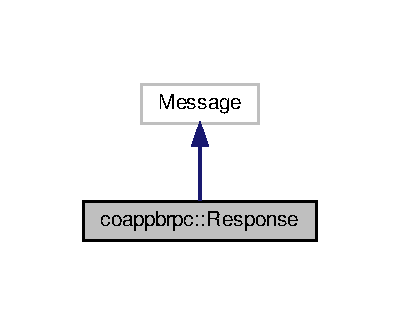
\includegraphics[width=192pt]{classcoappbrpc_1_1Response__inherit__graph}
\end{center}
\end{figure}


Collaboration diagram for coappbrpc\+:\+:Response\+:\nopagebreak
\begin{figure}[H]
\begin{center}
\leavevmode
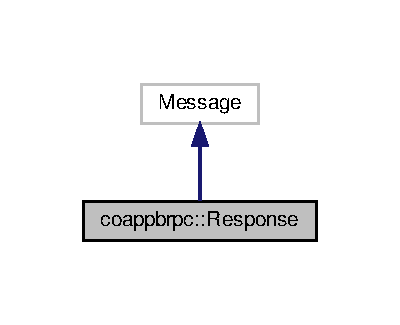
\includegraphics[width=192pt]{classcoappbrpc_1_1Response__coll__graph}
\end{center}
\end{figure}
\subsection*{Classes}
\begin{DoxyCompactItemize}
\item 
class \hyperlink{classcoappbrpc_1_1Response_1_1HasBitSetters}{Has\+Bit\+Setters}
\end{DoxyCompactItemize}
\subsection*{Public Member Functions}
\begin{DoxyCompactItemize}
\item 
\mbox{\Hypertarget{classcoappbrpc_1_1Response_a24904bb0f0787fce30908baa49edc716}\label{classcoappbrpc_1_1Response_a24904bb0f0787fce30908baa49edc716}} 
{\bfseries Response} (const \hyperlink{classcoappbrpc_1_1Response}{Response} \&from)
\item 
\mbox{\Hypertarget{classcoappbrpc_1_1Response_a61b7fa1a0db69410c56d5fe68780c672}\label{classcoappbrpc_1_1Response_a61b7fa1a0db69410c56d5fe68780c672}} 
\hyperlink{classcoappbrpc_1_1Response}{Response} \& {\bfseries operator=} (const \hyperlink{classcoappbrpc_1_1Response}{Response} \&from)
\item 
\mbox{\Hypertarget{classcoappbrpc_1_1Response_a8c4a23436a8b69a56ae78b77275b6c73}\label{classcoappbrpc_1_1Response_a8c4a23436a8b69a56ae78b77275b6c73}} 
void {\bfseries Swap} (\hyperlink{classcoappbrpc_1_1Response}{Response} $\ast$other)
\item 
\mbox{\Hypertarget{classcoappbrpc_1_1Response_a5376077cc9b1c06db82f865bbdde3393}\label{classcoappbrpc_1_1Response_a5376077cc9b1c06db82f865bbdde3393}} 
\hyperlink{classcoappbrpc_1_1Response}{Response} $\ast$ {\bfseries New} () const final
\item 
\mbox{\Hypertarget{classcoappbrpc_1_1Response_abd3c0c6327b76e29a6346ed2c4a3a799}\label{classcoappbrpc_1_1Response_abd3c0c6327b76e29a6346ed2c4a3a799}} 
\hyperlink{classcoappbrpc_1_1Response}{Response} $\ast$ {\bfseries New} (\+::google\+::protobuf\+::\+Arena $\ast$arena) const final
\item 
\mbox{\Hypertarget{classcoappbrpc_1_1Response_acd3ee1f81b27d08c0ffb155bdb9b3c1d}\label{classcoappbrpc_1_1Response_acd3ee1f81b27d08c0ffb155bdb9b3c1d}} 
void {\bfseries Copy\+From} (const \+::google\+::protobuf\+::\+Message \&from) final
\item 
\mbox{\Hypertarget{classcoappbrpc_1_1Response_ad20d2e5d879b0a4d6cd313b4da6618a1}\label{classcoappbrpc_1_1Response_ad20d2e5d879b0a4d6cd313b4da6618a1}} 
void {\bfseries Merge\+From} (const \+::google\+::protobuf\+::\+Message \&from) final
\item 
\mbox{\Hypertarget{classcoappbrpc_1_1Response_a3a27916c27b9cf8e3a437d1cbd1147c4}\label{classcoappbrpc_1_1Response_a3a27916c27b9cf8e3a437d1cbd1147c4}} 
void {\bfseries Copy\+From} (const \hyperlink{classcoappbrpc_1_1Response}{Response} \&from)
\item 
\mbox{\Hypertarget{classcoappbrpc_1_1Response_a9e65ff105d739a4f0fda6cf8ea0dd91f}\label{classcoappbrpc_1_1Response_a9e65ff105d739a4f0fda6cf8ea0dd91f}} 
void {\bfseries Merge\+From} (const \hyperlink{classcoappbrpc_1_1Response}{Response} \&from)
\item 
\mbox{\Hypertarget{classcoappbrpc_1_1Response_aa9b68b199f18a06cf3036430e6469ec2}\label{classcoappbrpc_1_1Response_aa9b68b199f18a06cf3036430e6469ec2}} 
void {\bfseries Clear} () final
\item 
\mbox{\Hypertarget{classcoappbrpc_1_1Response_a687c386d4428e724be5226c2c2c14479}\label{classcoappbrpc_1_1Response_a687c386d4428e724be5226c2c2c14479}} 
bool {\bfseries Is\+Initialized} () const final
\item 
\mbox{\Hypertarget{classcoappbrpc_1_1Response_a85bd1f7ae73c9dc3d370547a2794d56d}\label{classcoappbrpc_1_1Response_a85bd1f7ae73c9dc3d370547a2794d56d}} 
size\+\_\+t {\bfseries Byte\+Size\+Long} () const final
\item 
\mbox{\Hypertarget{classcoappbrpc_1_1Response_a338f6e91d6b68734fab073e37e842104}\label{classcoappbrpc_1_1Response_a338f6e91d6b68734fab073e37e842104}} 
bool {\bfseries Merge\+Partial\+From\+Coded\+Stream} (\+::google\+::protobuf\+::io\+::\+Coded\+Input\+Stream $\ast$input) final
\item 
\mbox{\Hypertarget{classcoappbrpc_1_1Response_a9245b3575fed37198c288936a47ba31c}\label{classcoappbrpc_1_1Response_a9245b3575fed37198c288936a47ba31c}} 
void {\bfseries Serialize\+With\+Cached\+Sizes} (\+::google\+::protobuf\+::io\+::\+Coded\+Output\+Stream $\ast$output) const final
\item 
\mbox{\Hypertarget{classcoappbrpc_1_1Response_a54352ac27422f88aec17253468593172}\label{classcoappbrpc_1_1Response_a54352ac27422f88aec17253468593172}} 
\+::google\+::protobuf\+::uint8 $\ast$ {\bfseries Internal\+Serialize\+With\+Cached\+Sizes\+To\+Array} (bool deterministic, \+::google\+::protobuf\+::uint8 $\ast$target) const final
\item 
\mbox{\Hypertarget{classcoappbrpc_1_1Response_a4eeebf1befe309f178185e3f8b4da3d1}\label{classcoappbrpc_1_1Response_a4eeebf1befe309f178185e3f8b4da3d1}} 
int {\bfseries Get\+Cached\+Size} () const final
\item 
\mbox{\Hypertarget{classcoappbrpc_1_1Response_a6724cea13f3ebabd4db02fead5bf0b12}\label{classcoappbrpc_1_1Response_a6724cea13f3ebabd4db02fead5bf0b12}} 
\+::google\+::protobuf\+::\+Metadata {\bfseries Get\+Metadata} () const final
\item 
\mbox{\Hypertarget{classcoappbrpc_1_1Response_a56714ff4c70fe010ca24ee2ab7c08b5a}\label{classcoappbrpc_1_1Response_a56714ff4c70fe010ca24ee2ab7c08b5a}} 
void {\bfseries clear\+\_\+version} ()
\item 
\mbox{\Hypertarget{classcoappbrpc_1_1Response_accf32df398527b83ac819ad6ddeb6bdf}\label{classcoappbrpc_1_1Response_accf32df398527b83ac819ad6ddeb6bdf}} 
const \+::std\+::string \& {\bfseries version} () const
\item 
\mbox{\Hypertarget{classcoappbrpc_1_1Response_a68bd09f954ddf08a00d478735e1c1eae}\label{classcoappbrpc_1_1Response_a68bd09f954ddf08a00d478735e1c1eae}} 
void {\bfseries set\+\_\+version} (const \+::std\+::string \&value)
\item 
\mbox{\Hypertarget{classcoappbrpc_1_1Response_a573b1dd1a43e6b6b6ad96a964ab576bb}\label{classcoappbrpc_1_1Response_a573b1dd1a43e6b6b6ad96a964ab576bb}} 
void {\bfseries set\+\_\+version} (const char $\ast$value)
\item 
\mbox{\Hypertarget{classcoappbrpc_1_1Response_aef97211cb8eebdef5b706d371098c9fe}\label{classcoappbrpc_1_1Response_aef97211cb8eebdef5b706d371098c9fe}} 
void {\bfseries set\+\_\+version} (const char $\ast$value, size\+\_\+t size)
\item 
\mbox{\Hypertarget{classcoappbrpc_1_1Response_a41691f43bfc03b7bd5703cc79a2e70a1}\label{classcoappbrpc_1_1Response_a41691f43bfc03b7bd5703cc79a2e70a1}} 
\+::std\+::string $\ast$ {\bfseries mutable\+\_\+version} ()
\item 
\mbox{\Hypertarget{classcoappbrpc_1_1Response_aab3845a6fca89242d3a507f1fb4ef411}\label{classcoappbrpc_1_1Response_aab3845a6fca89242d3a507f1fb4ef411}} 
\+::std\+::string $\ast$ {\bfseries release\+\_\+version} ()
\item 
\mbox{\Hypertarget{classcoappbrpc_1_1Response_a0f7068126473cbac403752d3be8c4374}\label{classcoappbrpc_1_1Response_a0f7068126473cbac403752d3be8c4374}} 
void {\bfseries set\+\_\+allocated\+\_\+version} (\+::std\+::string $\ast$version)
\item 
\mbox{\Hypertarget{classcoappbrpc_1_1Response_af8a767aac84ca69eb13656e15138fe77}\label{classcoappbrpc_1_1Response_af8a767aac84ca69eb13656e15138fe77}} 
void {\bfseries clear\+\_\+result} ()
\item 
\mbox{\Hypertarget{classcoappbrpc_1_1Response_a4a917b0e205dc60bf1a5d424fa5c4728}\label{classcoappbrpc_1_1Response_a4a917b0e205dc60bf1a5d424fa5c4728}} 
const \+::std\+::string \& {\bfseries result} () const
\item 
\mbox{\Hypertarget{classcoappbrpc_1_1Response_a4181db1a6c4b74f734693689d60d2edc}\label{classcoappbrpc_1_1Response_a4181db1a6c4b74f734693689d60d2edc}} 
void {\bfseries set\+\_\+result} (const \+::std\+::string \&value)
\item 
\mbox{\Hypertarget{classcoappbrpc_1_1Response_a232e7faf993df8c3c3adf40395091353}\label{classcoappbrpc_1_1Response_a232e7faf993df8c3c3adf40395091353}} 
void {\bfseries set\+\_\+result} (const char $\ast$value)
\item 
\mbox{\Hypertarget{classcoappbrpc_1_1Response_a6869735924f8020db2c8edf16ffea9a3}\label{classcoappbrpc_1_1Response_a6869735924f8020db2c8edf16ffea9a3}} 
void {\bfseries set\+\_\+result} (const void $\ast$value, size\+\_\+t size)
\item 
\mbox{\Hypertarget{classcoappbrpc_1_1Response_a3023ea3c2231705bd8ebd4754a0dd5aa}\label{classcoappbrpc_1_1Response_a3023ea3c2231705bd8ebd4754a0dd5aa}} 
\+::std\+::string $\ast$ {\bfseries mutable\+\_\+result} ()
\item 
\mbox{\Hypertarget{classcoappbrpc_1_1Response_ae35bcc72629ab642c373f331533d1ada}\label{classcoappbrpc_1_1Response_ae35bcc72629ab642c373f331533d1ada}} 
\+::std\+::string $\ast$ {\bfseries release\+\_\+result} ()
\item 
\mbox{\Hypertarget{classcoappbrpc_1_1Response_a3c01ab6b32b7411301538f447c1bc532}\label{classcoappbrpc_1_1Response_a3c01ab6b32b7411301538f447c1bc532}} 
void {\bfseries set\+\_\+allocated\+\_\+result} (\+::std\+::string $\ast$result)
\item 
\mbox{\Hypertarget{classcoappbrpc_1_1Response_a6a51678205f747030d38bfef138d705e}\label{classcoappbrpc_1_1Response_a6a51678205f747030d38bfef138d705e}} 
bool {\bfseries has\+\_\+error} () const
\item 
\mbox{\Hypertarget{classcoappbrpc_1_1Response_ac226b43c4a08c6fcb8b68d68c20b60ab}\label{classcoappbrpc_1_1Response_ac226b43c4a08c6fcb8b68d68c20b60ab}} 
void {\bfseries clear\+\_\+error} ()
\item 
\mbox{\Hypertarget{classcoappbrpc_1_1Response_a42b9742feb5e666028ef646e1854523f}\label{classcoappbrpc_1_1Response_a42b9742feb5e666028ef646e1854523f}} 
const \+::\hyperlink{classcoappbrpc_1_1Error}{coappbrpc\+::\+Error} \& {\bfseries error} () const
\item 
\mbox{\Hypertarget{classcoappbrpc_1_1Response_a024c37fee8ee34f3daaa45ff55d39e84}\label{classcoappbrpc_1_1Response_a024c37fee8ee34f3daaa45ff55d39e84}} 
\+::\hyperlink{classcoappbrpc_1_1Error}{coappbrpc\+::\+Error} $\ast$ {\bfseries release\+\_\+error} ()
\item 
\mbox{\Hypertarget{classcoappbrpc_1_1Response_a48c1ac0df3977860dd2531d6c8429ad9}\label{classcoappbrpc_1_1Response_a48c1ac0df3977860dd2531d6c8429ad9}} 
\+::\hyperlink{classcoappbrpc_1_1Error}{coappbrpc\+::\+Error} $\ast$ {\bfseries mutable\+\_\+error} ()
\item 
\mbox{\Hypertarget{classcoappbrpc_1_1Response_aa536601e1f7dcd45fd6fccffa6e15ca9}\label{classcoappbrpc_1_1Response_aa536601e1f7dcd45fd6fccffa6e15ca9}} 
void {\bfseries set\+\_\+allocated\+\_\+error} (\+::\hyperlink{classcoappbrpc_1_1Error}{coappbrpc\+::\+Error} $\ast$error)
\item 
\mbox{\Hypertarget{classcoappbrpc_1_1Response_a205de4d84232bde24326a6274d9b8acf}\label{classcoappbrpc_1_1Response_a205de4d84232bde24326a6274d9b8acf}} 
void {\bfseries clear\+\_\+id} ()
\item 
\mbox{\Hypertarget{classcoappbrpc_1_1Response_a89389be177aab69c762aaf218821bb32}\label{classcoappbrpc_1_1Response_a89389be177aab69c762aaf218821bb32}} 
\+::google\+::protobuf\+::int32 {\bfseries id} () const
\item 
\mbox{\Hypertarget{classcoappbrpc_1_1Response_af23aeab5cc0df75a26500f87e9942cee}\label{classcoappbrpc_1_1Response_af23aeab5cc0df75a26500f87e9942cee}} 
void {\bfseries set\+\_\+id} (\+::google\+::protobuf\+::int32 value)
\end{DoxyCompactItemize}
\subsection*{Static Public Member Functions}
\begin{DoxyCompactItemize}
\item 
\mbox{\Hypertarget{classcoappbrpc_1_1Response_aee7d5c409330433ba6061269965d7dd5}\label{classcoappbrpc_1_1Response_aee7d5c409330433ba6061269965d7dd5}} 
static const \+::google\+::protobuf\+::\+Descriptor $\ast$ {\bfseries descriptor} ()
\item 
\mbox{\Hypertarget{classcoappbrpc_1_1Response_a61ecfdb459c74f3ce536b878d5759007}\label{classcoappbrpc_1_1Response_a61ecfdb459c74f3ce536b878d5759007}} 
static const \hyperlink{classcoappbrpc_1_1Response}{Response} \& {\bfseries default\+\_\+instance} ()
\item 
\mbox{\Hypertarget{classcoappbrpc_1_1Response_a07665b433b0600546098d98a0afb52d7}\label{classcoappbrpc_1_1Response_a07665b433b0600546098d98a0afb52d7}} 
static void {\bfseries Init\+As\+Default\+Instance} ()
\item 
\mbox{\Hypertarget{classcoappbrpc_1_1Response_a0551fd997235f3871029b45c170b70ed}\label{classcoappbrpc_1_1Response_a0551fd997235f3871029b45c170b70ed}} 
static const \hyperlink{classcoappbrpc_1_1Response}{Response} $\ast$ {\bfseries internal\+\_\+default\+\_\+instance} ()
\end{DoxyCompactItemize}
\subsection*{Static Public Attributes}
\begin{DoxyCompactItemize}
\item 
static constexpr int {\bfseries k\+Index\+In\+File\+Messages}
\item 
\mbox{\Hypertarget{classcoappbrpc_1_1Response_a419e8532ffd97e6bab8cdcf27d31203f}\label{classcoappbrpc_1_1Response_a419e8532ffd97e6bab8cdcf27d31203f}} 
static const int {\bfseries k\+Version\+Field\+Number} = 1
\item 
\mbox{\Hypertarget{classcoappbrpc_1_1Response_a0132ee8e4087c92e607c548d46474964}\label{classcoappbrpc_1_1Response_a0132ee8e4087c92e607c548d46474964}} 
static const int {\bfseries k\+Result\+Field\+Number} = 2
\item 
\mbox{\Hypertarget{classcoappbrpc_1_1Response_ae7fdafbc86f89e117a6760c67eb3d9c2}\label{classcoappbrpc_1_1Response_ae7fdafbc86f89e117a6760c67eb3d9c2}} 
static const int {\bfseries k\+Error\+Field\+Number} = 3
\item 
\mbox{\Hypertarget{classcoappbrpc_1_1Response_ab1099b6e840365727c22e8bbe79f979a}\label{classcoappbrpc_1_1Response_ab1099b6e840365727c22e8bbe79f979a}} 
static const int {\bfseries k\+Id\+Field\+Number} = 4
\end{DoxyCompactItemize}
\subsection*{Friends}
\begin{DoxyCompactItemize}
\item 
\mbox{\Hypertarget{classcoappbrpc_1_1Response_a65c087bf06ded9c9be363691f7b7bafa}\label{classcoappbrpc_1_1Response_a65c087bf06ded9c9be363691f7b7bafa}} 
struct {\bfseries \+::\+Table\+Struct\+\_\+\+Msg\+Schema\+\_\+2eproto}
\item 
\mbox{\Hypertarget{classcoappbrpc_1_1Response_abd2d29760e9668486937c4d6f11784e6}\label{classcoappbrpc_1_1Response_abd2d29760e9668486937c4d6f11784e6}} 
void {\bfseries swap} (\hyperlink{classcoappbrpc_1_1Response}{Response} \&a, \hyperlink{classcoappbrpc_1_1Response}{Response} \&b)
\end{DoxyCompactItemize}


\subsection{Member Data Documentation}
\mbox{\Hypertarget{classcoappbrpc_1_1Response_ae8e167e80cc311e00980ac897decdceb}\label{classcoappbrpc_1_1Response_ae8e167e80cc311e00980ac897decdceb}} 
\index{coappbrpc\+::\+Response@{coappbrpc\+::\+Response}!k\+Index\+In\+File\+Messages@{k\+Index\+In\+File\+Messages}}
\index{k\+Index\+In\+File\+Messages@{k\+Index\+In\+File\+Messages}!coappbrpc\+::\+Response@{coappbrpc\+::\+Response}}
\subsubsection{\texorpdfstring{k\+Index\+In\+File\+Messages}{kIndexInFileMessages}}
{\footnotesize\ttfamily constexpr int coappbrpc\+::\+Response\+::k\+Index\+In\+File\+Messages\hspace{0.3cm}{\ttfamily [static]}}

{\bfseries Initial value\+:}
\begin{DoxyCode}
=
    2
\end{DoxyCode}


The documentation for this class was generated from the following files\+:\begin{DoxyCompactItemize}
\item 
build/proto/Msg\+Schema.\+pb.\+h\item 
build/proto/Msg\+Schema.\+pb.\+cc\end{DoxyCompactItemize}

\hypertarget{classcoappbrpc_1_1ResponseDefaultTypeInternal}{}\section{coappbrpc\+:\+:Response\+Default\+Type\+Internal Class Reference}
\label{classcoappbrpc_1_1ResponseDefaultTypeInternal}\index{coappbrpc\+::\+Response\+Default\+Type\+Internal@{coappbrpc\+::\+Response\+Default\+Type\+Internal}}
\subsection*{Public Attributes}
\begin{DoxyCompactItemize}
\item 
\mbox{\Hypertarget{classcoappbrpc_1_1ResponseDefaultTypeInternal_a2682abc1502e4594ce2ef83ca88e219d}\label{classcoappbrpc_1_1ResponseDefaultTypeInternal_a2682abc1502e4594ce2ef83ca88e219d}} 
\+::google\+::protobuf\+::internal\+::\+Explicitly\+Constructed$<$ \hyperlink{classcoappbrpc_1_1Response}{Response} $>$ {\bfseries \+\_\+instance}
\end{DoxyCompactItemize}


The documentation for this class was generated from the following file\+:\begin{DoxyCompactItemize}
\item 
build/proto/Msg\+Schema.\+pb.\+cc\end{DoxyCompactItemize}

\hypertarget{classcoappbrpc_1_1RpcClient}{}\section{coappbrpc\+:\+:Rpc\+Client Class Reference}
\label{classcoappbrpc_1_1RpcClient}\index{coappbrpc\+::\+Rpc\+Client@{coappbrpc\+::\+Rpc\+Client}}


This class contains methods to run client, set responses, get responses, setup server addresses and execute function which is called from client stubs.  




{\ttfamily \#include $<$Rpc\+Client.\+h$>$}

\subsection*{Public Member Functions}
\begin{DoxyCompactItemize}
\item 
\mbox{\Hypertarget{classcoappbrpc_1_1RpcClient_a9b90b3ba0fef5ebd90748e454c1c7fd9}\label{classcoappbrpc_1_1RpcClient_a9b90b3ba0fef5ebd90748e454c1c7fd9}} 
virtual \hyperlink{classcoappbrpc_1_1RpcClient_a9b90b3ba0fef5ebd90748e454c1c7fd9}{$\sim$\+Rpc\+Client} ()
\begin{DoxyCompactList}\small\item\em R\+PC Client Destructor. \end{DoxyCompactList}\item 
\mbox{\Hypertarget{classcoappbrpc_1_1RpcClient_a19f14a9f5ac45332f1656c0ab033dc09}\label{classcoappbrpc_1_1RpcClient_a19f14a9f5ac45332f1656c0ab033dc09}} 
void \hyperlink{classcoappbrpc_1_1RpcClient_a19f14a9f5ac45332f1656c0ab033dc09}{run\+Client} ()
\begin{DoxyCompactList}\small\item\em Creates data structure to be sent to Coap Client and executes coap client\textquotesingle{}s execute\+Client function. \end{DoxyCompactList}\item 
void \hyperlink{classcoappbrpc_1_1RpcClient_a0f08b63838a62377d4470eb2a0259178}{set\+Response} (string)
\begin{DoxyCompactList}\small\item\em Setter function to store response to m\+\_\+response variable. \end{DoxyCompactList}\item 
\mbox{\Hypertarget{classcoappbrpc_1_1RpcClient_ac79e3b2a76335a214cbe1c6f169d46c2}\label{classcoappbrpc_1_1RpcClient_ac79e3b2a76335a214cbe1c6f169d46c2}} 
string \hyperlink{classcoappbrpc_1_1RpcClient_ac79e3b2a76335a214cbe1c6f169d46c2}{get\+Response} ()
\begin{DoxyCompactList}\small\item\em Getter function to get response stored in m\+\_\+response variable. \end{DoxyCompactList}\item 
void \hyperlink{classcoappbrpc_1_1RpcClient_a69755d690a7f2d6373e191d359e48986}{set\+Server\+Addr} (string, string)
\begin{DoxyCompactList}\small\item\em Setter function to store ip address and port to m\+\_\+address and m\+\_\+port respectively. \end{DoxyCompactList}\item 
Response \hyperlink{classcoappbrpc_1_1RpcClient_afe2dc0caa49442db4898379d040c8b64}{exec\+Func} (string, string, string, string)
\begin{DoxyCompactList}\small\item\em Creates protocol buffer data structure containing version number, services, methods, method parameters, unique Random ids. Then it serializes the data into string and stores it in m\+\_\+payload variable. This function calls run\+Client function. And after it receives response, it returns response as type Response. \end{DoxyCompactList}\end{DoxyCompactItemize}
\subsection*{Static Public Member Functions}
\begin{DoxyCompactItemize}
\item 
\mbox{\Hypertarget{classcoappbrpc_1_1RpcClient_a36bb0e75fae00e4ea9e643d8c1b16f5c}\label{classcoappbrpc_1_1RpcClient_a36bb0e75fae00e4ea9e643d8c1b16f5c}} 
static \hyperlink{classcoappbrpc_1_1RpcClient}{Rpc\+Client} $\ast$ \hyperlink{classcoappbrpc_1_1RpcClient_a36bb0e75fae00e4ea9e643d8c1b16f5c}{get\+Instance} ()
\begin{DoxyCompactList}\small\item\em getting new client\+R\+PC instance \end{DoxyCompactList}\end{DoxyCompactItemize}


\subsection{Detailed Description}
This class contains methods to run client, set responses, get responses, setup server addresses and execute function which is called from client stubs. 

\subsection{Member Function Documentation}
\mbox{\Hypertarget{classcoappbrpc_1_1RpcClient_afe2dc0caa49442db4898379d040c8b64}\label{classcoappbrpc_1_1RpcClient_afe2dc0caa49442db4898379d040c8b64}} 
\index{coappbrpc\+::\+Rpc\+Client@{coappbrpc\+::\+Rpc\+Client}!exec\+Func@{exec\+Func}}
\index{exec\+Func@{exec\+Func}!coappbrpc\+::\+Rpc\+Client@{coappbrpc\+::\+Rpc\+Client}}
\subsubsection{\texorpdfstring{exec\+Func()}{execFunc()}}
{\footnotesize\ttfamily Response coappbrpc\+::\+Rpc\+Client\+::exec\+Func (\begin{DoxyParamCaption}\item[{string}]{vers,  }\item[{string}]{service\+Name,  }\item[{string}]{method,  }\item[{string}]{msg }\end{DoxyParamCaption})}



Creates protocol buffer data structure containing version number, services, methods, method parameters, unique Random ids. Then it serializes the data into string and stores it in m\+\_\+payload variable. This function calls run\+Client function. And after it receives response, it returns response as type Response. 


\begin{DoxyParams}{Parameters}
{\em vers} & version number defined in \hyperlink{Config_8h}{Config.\+h} file \\
\hline
{\em service\+Name} & Name of Service to be used for R\+PC calls \\
\hline
{\em method} & Method name to be called when executing R\+PC \\
\hline
{\em msg} & Serialized message to be sent to Server, contains defination of various parameters to a particular method. \\
\hline
\end{DoxyParams}
\mbox{\Hypertarget{classcoappbrpc_1_1RpcClient_a0f08b63838a62377d4470eb2a0259178}\label{classcoappbrpc_1_1RpcClient_a0f08b63838a62377d4470eb2a0259178}} 
\index{coappbrpc\+::\+Rpc\+Client@{coappbrpc\+::\+Rpc\+Client}!set\+Response@{set\+Response}}
\index{set\+Response@{set\+Response}!coappbrpc\+::\+Rpc\+Client@{coappbrpc\+::\+Rpc\+Client}}
\subsubsection{\texorpdfstring{set\+Response()}{setResponse()}}
{\footnotesize\ttfamily void coappbrpc\+::\+Rpc\+Client\+::set\+Response (\begin{DoxyParamCaption}\item[{string}]{resp }\end{DoxyParamCaption})}



Setter function to store response to m\+\_\+response variable. 


\begin{DoxyParams}{Parameters}
{\em resp} & Response string to be stored in member variable m\+\_\+response \\
\hline
\end{DoxyParams}
\mbox{\Hypertarget{classcoappbrpc_1_1RpcClient_a69755d690a7f2d6373e191d359e48986}\label{classcoappbrpc_1_1RpcClient_a69755d690a7f2d6373e191d359e48986}} 
\index{coappbrpc\+::\+Rpc\+Client@{coappbrpc\+::\+Rpc\+Client}!set\+Server\+Addr@{set\+Server\+Addr}}
\index{set\+Server\+Addr@{set\+Server\+Addr}!coappbrpc\+::\+Rpc\+Client@{coappbrpc\+::\+Rpc\+Client}}
\subsubsection{\texorpdfstring{set\+Server\+Addr()}{setServerAddr()}}
{\footnotesize\ttfamily void coappbrpc\+::\+Rpc\+Client\+::set\+Server\+Addr (\begin{DoxyParamCaption}\item[{string}]{ip\+Addr,  }\item[{string}]{port }\end{DoxyParamCaption})}



Setter function to store ip address and port to m\+\_\+address and m\+\_\+port respectively. 


\begin{DoxyParams}{Parameters}
{\em ip\+Addr} & Ip Address may be I\+Pv4 or I\+Pv6 to be stored in m\+\_\+address variable \\
\hline
{\em port} & Port no to be stored in m\+\_\+port variable \\
\hline
\end{DoxyParams}


The documentation for this class was generated from the following files\+:\begin{DoxyCompactItemize}
\item 
include/\hyperlink{RpcClient_8h}{Rpc\+Client.\+h}\item 
src/\hyperlink{RpcClient_8cc}{Rpc\+Client.\+cc}\end{DoxyCompactItemize}

\hypertarget{classcoappbrpc_1_1RpcMethod}{}\section{coappbrpc\+:\+:Rpc\+Method Class Reference}
\label{classcoappbrpc_1_1RpcMethod}\index{coappbrpc\+::\+Rpc\+Method@{coappbrpc\+::\+Rpc\+Method}}
\subsection*{Public Member Functions}
\begin{DoxyCompactItemize}
\item 
\mbox{\Hypertarget{classcoappbrpc_1_1RpcMethod_af48f7fb693239a6b0359dc083b855a93}\label{classcoappbrpc_1_1RpcMethod_af48f7fb693239a6b0359dc083b855a93}} 
{\bfseries Rpc\+Method} (const Method\+Descriptor $\ast$\hyperlink{classcoappbrpc_1_1RpcMethod_a52010a290e164174ca969c8904d1f3da}{descriptor}, const Message $\ast$\hyperlink{classcoappbrpc_1_1RpcMethod_ac8d0272f2480f41d10c91c023708b8f8}{request}, const Message $\ast$\hyperlink{classcoappbrpc_1_1RpcMethod_a95a64db4546c8e418232fafa297fc9a5}{response})
\end{DoxyCompactItemize}
\subsection*{Public Attributes}
\begin{DoxyCompactItemize}
\item 
const Method\+Descriptor $\ast$ \hyperlink{classcoappbrpc_1_1RpcMethod_a52010a290e164174ca969c8904d1f3da}{descriptor}
\item 
const Message $\ast$ \hyperlink{classcoappbrpc_1_1RpcMethod_ac8d0272f2480f41d10c91c023708b8f8}{request}
\item 
const Message $\ast$ \hyperlink{classcoappbrpc_1_1RpcMethod_a95a64db4546c8e418232fafa297fc9a5}{response}
\end{DoxyCompactItemize}


\subsection{Member Data Documentation}
\mbox{\Hypertarget{classcoappbrpc_1_1RpcMethod_a52010a290e164174ca969c8904d1f3da}\label{classcoappbrpc_1_1RpcMethod_a52010a290e164174ca969c8904d1f3da}} 
\index{coappbrpc\+::\+Rpc\+Method@{coappbrpc\+::\+Rpc\+Method}!descriptor@{descriptor}}
\index{descriptor@{descriptor}!coappbrpc\+::\+Rpc\+Method@{coappbrpc\+::\+Rpc\+Method}}
\subsubsection{\texorpdfstring{descriptor}{descriptor}}
{\footnotesize\ttfamily const Method\+Descriptor$\ast$ coappbrpc\+::\+Rpc\+Method\+::descriptor}

method descriptor \mbox{\Hypertarget{classcoappbrpc_1_1RpcMethod_ac8d0272f2480f41d10c91c023708b8f8}\label{classcoappbrpc_1_1RpcMethod_ac8d0272f2480f41d10c91c023708b8f8}} 
\index{coappbrpc\+::\+Rpc\+Method@{coappbrpc\+::\+Rpc\+Method}!request@{request}}
\index{request@{request}!coappbrpc\+::\+Rpc\+Method@{coappbrpc\+::\+Rpc\+Method}}
\subsubsection{\texorpdfstring{request}{request}}
{\footnotesize\ttfamily const Message$\ast$ coappbrpc\+::\+Rpc\+Method\+::request}

parameters \mbox{\Hypertarget{classcoappbrpc_1_1RpcMethod_a95a64db4546c8e418232fafa297fc9a5}\label{classcoappbrpc_1_1RpcMethod_a95a64db4546c8e418232fafa297fc9a5}} 
\index{coappbrpc\+::\+Rpc\+Method@{coappbrpc\+::\+Rpc\+Method}!response@{response}}
\index{response@{response}!coappbrpc\+::\+Rpc\+Method@{coappbrpc\+::\+Rpc\+Method}}
\subsubsection{\texorpdfstring{response}{response}}
{\footnotesize\ttfamily const Message$\ast$ coappbrpc\+::\+Rpc\+Method\+::response}

result 

The documentation for this class was generated from the following file\+:\begin{DoxyCompactItemize}
\item 
include/\hyperlink{RpcMethod_8h}{Rpc\+Method.\+h}\end{DoxyCompactItemize}

\hypertarget{classcoappbrpc_1_1RpcServer}{}\section{coappbrpc\+:\+:Rpc\+Server Class Reference}
\label{classcoappbrpc_1_1RpcServer}\index{coappbrpc\+::\+Rpc\+Server@{coappbrpc\+::\+Rpc\+Server}}


This class consists of methods to register\+Service and run\+Server.  




{\ttfamily \#include $<$Rpc\+Server.\+h$>$}

\subsection*{Public Member Functions}
\begin{DoxyCompactItemize}
\item 
\mbox{\Hypertarget{classcoappbrpc_1_1RpcServer_af204829e600b25eebbe1b2f25998bf3a}\label{classcoappbrpc_1_1RpcServer_af204829e600b25eebbe1b2f25998bf3a}} 
\hyperlink{classcoappbrpc_1_1RpcServer_af204829e600b25eebbe1b2f25998bf3a}{Rpc\+Server} ()
\begin{DoxyCompactList}\small\item\em Constructor function which sets variable \char`\"{}running\char`\"{} to false for every instance. \end{DoxyCompactList}\item 
\mbox{\Hypertarget{classcoappbrpc_1_1RpcServer_a6fdde51aa522ed81525990fe2d969380}\label{classcoappbrpc_1_1RpcServer_a6fdde51aa522ed81525990fe2d969380}} 
virtual \hyperlink{classcoappbrpc_1_1RpcServer_a6fdde51aa522ed81525990fe2d969380}{$\sim$\+Rpc\+Server} ()
\begin{DoxyCompactList}\small\item\em Destructor Function. \end{DoxyCompactList}\item 
\mbox{\Hypertarget{classcoappbrpc_1_1RpcServer_a7658f607ecc19f8c05082363ffd5cd54}\label{classcoappbrpc_1_1RpcServer_a7658f607ecc19f8c05082363ffd5cd54}} 
int \hyperlink{classcoappbrpc_1_1RpcServer_a7658f607ecc19f8c05082363ffd5cd54}{start} ()
\begin{DoxyCompactList}\small\item\em this function starts the coap server First it checks if the R\+PC server is running or not. Then it creates a coap context, handles coap resresources and runs the coap server. \end{DoxyCompactList}\item 
\mbox{\Hypertarget{classcoappbrpc_1_1RpcServer_a93a8e554d0e52b30b79ca8077f040bb2}\label{classcoappbrpc_1_1RpcServer_a93a8e554d0e52b30b79ca8077f040bb2}} 
bool \hyperlink{classcoappbrpc_1_1RpcServer_a93a8e554d0e52b30b79ca8077f040bb2}{stop} (int)
\begin{DoxyCompactList}\small\item\em This function stops the coap server It stops coap server, free coap context, cleanup memory allocations and resets running flag to false. \end{DoxyCompactList}\item 
\mbox{\Hypertarget{classcoappbrpc_1_1RpcServer_a453e2eb88b54439a1ba249ee66ee912e}\label{classcoappbrpc_1_1RpcServer_a453e2eb88b54439a1ba249ee66ee912e}} 
void \hyperlink{classcoappbrpc_1_1RpcServer_a453e2eb88b54439a1ba249ee66ee912e}{run\+Server} ()
\begin{DoxyCompactList}\small\item\em default run\+Server function which overloads if ip address and port is not given. \end{DoxyCompactList}\item 
void \hyperlink{classcoappbrpc_1_1RpcServer_ac1742b534bbb7c0b054c40346c876cf5}{run\+Server} (const char $\ast$, const char $\ast$)
\begin{DoxyCompactList}\small\item\em Setter function to set server ip address and port number and calls for \char`\"{}start\char`\"{} function to run Server. Default address is localhost and port is 5683. Function overloading used for handling default values incase parameters are not passed. \end{DoxyCompactList}\item 
void \hyperlink{classcoappbrpc_1_1RpcServer_acc9877a9bfff6783aa0261942d2917c2}{register\+Service} (Service $\ast$service)
\begin{DoxyCompactList}\small\item\em This function calls handle\+Reg\+Service. \end{DoxyCompactList}\end{DoxyCompactItemize}
\subsection*{Public Attributes}
\begin{DoxyCompactItemize}
\item 
coap\+\_\+context\+\_\+t $\ast$ \hyperlink{classcoappbrpc_1_1RpcServer_a34a0db66e265d8986dea6d9e360a7ca3}{ctx} = nullptr
\item 
const char $\ast$ \hyperlink{classcoappbrpc_1_1RpcServer_a9fec802c5d77b168560d14b73fc988e1}{port}
\item 
const char $\ast$ \hyperlink{classcoappbrpc_1_1RpcServer_a14953d39d8e53a7f3dcffde2d15734d0}{server\+Addr}
\item 
bool \hyperlink{classcoappbrpc_1_1RpcServer_a5110ce6a1447e421359982aff15744e2}{running} = false
\end{DoxyCompactItemize}


\subsection{Detailed Description}
This class consists of methods to register\+Service and run\+Server. 

\subsection{Member Function Documentation}
\mbox{\Hypertarget{classcoappbrpc_1_1RpcServer_acc9877a9bfff6783aa0261942d2917c2}\label{classcoappbrpc_1_1RpcServer_acc9877a9bfff6783aa0261942d2917c2}} 
\index{coappbrpc\+::\+Rpc\+Server@{coappbrpc\+::\+Rpc\+Server}!register\+Service@{register\+Service}}
\index{register\+Service@{register\+Service}!coappbrpc\+::\+Rpc\+Server@{coappbrpc\+::\+Rpc\+Server}}
\subsubsection{\texorpdfstring{register\+Service()}{registerService()}}
{\footnotesize\ttfamily void coappbrpc\+::\+Rpc\+Server\+::register\+Service (\begin{DoxyParamCaption}\item[{Service $\ast$}]{service }\end{DoxyParamCaption})}



This function calls handle\+Reg\+Service. 


\begin{DoxyParams}{Parameters}
{\em service} & Type Service defined in protobuf services \\
\hline
\end{DoxyParams}
\mbox{\Hypertarget{classcoappbrpc_1_1RpcServer_ac1742b534bbb7c0b054c40346c876cf5}\label{classcoappbrpc_1_1RpcServer_ac1742b534bbb7c0b054c40346c876cf5}} 
\index{coappbrpc\+::\+Rpc\+Server@{coappbrpc\+::\+Rpc\+Server}!run\+Server@{run\+Server}}
\index{run\+Server@{run\+Server}!coappbrpc\+::\+Rpc\+Server@{coappbrpc\+::\+Rpc\+Server}}
\subsubsection{\texorpdfstring{run\+Server()}{runServer()}}
{\footnotesize\ttfamily void coappbrpc\+::\+Rpc\+Server\+::run\+Server (\begin{DoxyParamCaption}\item[{const char $\ast$}]{ip\+Addr,  }\item[{const char $\ast$}]{port }\end{DoxyParamCaption})}



Setter function to set server ip address and port number and calls for \char`\"{}start\char`\"{} function to run Server. Default address is localhost and port is 5683. Function overloading used for handling default values incase parameters are not passed. 


\begin{DoxyParams}{Parameters}
{\em ip\+Addr} & Ip Address reference variable \\
\hline
{\em port} & port reference variable \\
\hline
\end{DoxyParams}


\subsection{Member Data Documentation}
\mbox{\Hypertarget{classcoappbrpc_1_1RpcServer_a34a0db66e265d8986dea6d9e360a7ca3}\label{classcoappbrpc_1_1RpcServer_a34a0db66e265d8986dea6d9e360a7ca3}} 
\index{coappbrpc\+::\+Rpc\+Server@{coappbrpc\+::\+Rpc\+Server}!ctx@{ctx}}
\index{ctx@{ctx}!coappbrpc\+::\+Rpc\+Server@{coappbrpc\+::\+Rpc\+Server}}
\subsubsection{\texorpdfstring{ctx}{ctx}}
{\footnotesize\ttfamily coap\+\_\+context\+\_\+t$\ast$ coappbrpc\+::\+Rpc\+Server\+::ctx = nullptr}

Coap context pointer variable \mbox{\Hypertarget{classcoappbrpc_1_1RpcServer_a9fec802c5d77b168560d14b73fc988e1}\label{classcoappbrpc_1_1RpcServer_a9fec802c5d77b168560d14b73fc988e1}} 
\index{coappbrpc\+::\+Rpc\+Server@{coappbrpc\+::\+Rpc\+Server}!port@{port}}
\index{port@{port}!coappbrpc\+::\+Rpc\+Server@{coappbrpc\+::\+Rpc\+Server}}
\subsubsection{\texorpdfstring{port}{port}}
{\footnotesize\ttfamily const char$\ast$ coappbrpc\+::\+Rpc\+Server\+::port}

const char variable to store port no \mbox{\Hypertarget{classcoappbrpc_1_1RpcServer_a5110ce6a1447e421359982aff15744e2}\label{classcoappbrpc_1_1RpcServer_a5110ce6a1447e421359982aff15744e2}} 
\index{coappbrpc\+::\+Rpc\+Server@{coappbrpc\+::\+Rpc\+Server}!running@{running}}
\index{running@{running}!coappbrpc\+::\+Rpc\+Server@{coappbrpc\+::\+Rpc\+Server}}
\subsubsection{\texorpdfstring{running}{running}}
{\footnotesize\ttfamily bool coappbrpc\+::\+Rpc\+Server\+::running = false}

boolean variable to flag whether R\+PC is running or not \mbox{\Hypertarget{classcoappbrpc_1_1RpcServer_a14953d39d8e53a7f3dcffde2d15734d0}\label{classcoappbrpc_1_1RpcServer_a14953d39d8e53a7f3dcffde2d15734d0}} 
\index{coappbrpc\+::\+Rpc\+Server@{coappbrpc\+::\+Rpc\+Server}!server\+Addr@{server\+Addr}}
\index{server\+Addr@{server\+Addr}!coappbrpc\+::\+Rpc\+Server@{coappbrpc\+::\+Rpc\+Server}}
\subsubsection{\texorpdfstring{server\+Addr}{serverAddr}}
{\footnotesize\ttfamily const char$\ast$ coappbrpc\+::\+Rpc\+Server\+::server\+Addr}

const char variable to store IP address 

The documentation for this class was generated from the following files\+:\begin{DoxyCompactItemize}
\item 
include/\hyperlink{RpcServer_8h}{Rpc\+Server.\+h}\item 
src/\hyperlink{RpcServer_8cc}{Rpc\+Server.\+cc}\end{DoxyCompactItemize}

\hypertarget{classcoappbrpc_1_1RpcService}{}\section{coappbrpc\+:\+:Rpc\+Service Class Reference}
\label{classcoappbrpc_1_1RpcService}\index{coappbrpc\+::\+Rpc\+Service@{coappbrpc\+::\+Rpc\+Service}}


This class defines service for remote calls. It has methods for adding rpc methods, getting methods, validating if method exists.  




{\ttfamily \#include $<$Rpc\+Service.\+h$>$}

\subsection*{Public Member Functions}
\begin{DoxyCompactItemize}
\item 
\hyperlink{classcoappbrpc_1_1RpcService_a66c75fc19a62dbf650f4dc5080d15bfa}{Rpc\+Service} (Service $\ast$service)
\begin{DoxyCompactList}\small\item\em This is constructor function that scans service description, gets request prototype \& response prototype,loops over numbers of available methods and calls add\+Method function for each methods defined. \end{DoxyCompactList}\item 
\mbox{\Hypertarget{classcoappbrpc_1_1RpcService_a3cb969b5056dc0d5264552a16c1d244f}\label{classcoappbrpc_1_1RpcService_a3cb969b5056dc0d5264552a16c1d244f}} 
void \hyperlink{classcoappbrpc_1_1RpcService_a3cb969b5056dc0d5264552a16c1d244f}{add\+Method} (const \hyperlink{classcoappbrpc_1_1RpcMethod}{Rpc\+Method} \&method, const string \&method\+Name)
\begin{DoxyCompactList}\small\item\em This function is setter function that adds method\+Name to \+\_\+method array of type map$<$string, Rpc\+Method$>$ \end{DoxyCompactList}\item 
\mbox{\Hypertarget{classcoappbrpc_1_1RpcService_afdbb7a187c602fc830c5b3101e6b2e35}\label{classcoappbrpc_1_1RpcService_afdbb7a187c602fc830c5b3101e6b2e35}} 
const \hyperlink{classcoappbrpc_1_1RpcMethod}{Rpc\+Method} $\ast$ \hyperlink{classcoappbrpc_1_1RpcService_afdbb7a187c602fc830c5b3101e6b2e35}{get\+Method} (const string \&method\+Name) const
\begin{DoxyCompactList}\small\item\em This is getter function that gets the methods if they exist in \+\_\+method array. \end{DoxyCompactList}\item 
\mbox{\Hypertarget{classcoappbrpc_1_1RpcService_a0c7f4041e49a3d4e0abd6eb9aad9691d}\label{classcoappbrpc_1_1RpcService_a0c7f4041e49a3d4e0abd6eb9aad9691d}} 
bool \hyperlink{classcoappbrpc_1_1RpcService_a0c7f4041e49a3d4e0abd6eb9aad9691d}{is\+Exist\+Method} (const string \&method\+Name) const
\begin{DoxyCompactList}\small\item\em This function is for validating if the method name exists or not. \end{DoxyCompactList}\end{DoxyCompactItemize}
\subsection*{Public Attributes}
\begin{DoxyCompactItemize}
\item 
Service $\ast$ \hyperlink{classcoappbrpc_1_1RpcService_ab79621dd2a66b154352101e64f2dfefa}{\+\_\+service}
\item 
map$<$ string, \hyperlink{classcoappbrpc_1_1RpcMethod}{Rpc\+Method} $>$ \hyperlink{classcoappbrpc_1_1RpcService_a14b0b1bae1efc308e1c61d7737b7c4ac}{\+\_\+methods}
\end{DoxyCompactItemize}


\subsection{Detailed Description}
This class defines service for remote calls. It has methods for adding rpc methods, getting methods, validating if method exists. 

\subsection{Constructor \& Destructor Documentation}
\mbox{\Hypertarget{classcoappbrpc_1_1RpcService_a66c75fc19a62dbf650f4dc5080d15bfa}\label{classcoappbrpc_1_1RpcService_a66c75fc19a62dbf650f4dc5080d15bfa}} 
\index{coappbrpc\+::\+Rpc\+Service@{coappbrpc\+::\+Rpc\+Service}!Rpc\+Service@{Rpc\+Service}}
\index{Rpc\+Service@{Rpc\+Service}!coappbrpc\+::\+Rpc\+Service@{coappbrpc\+::\+Rpc\+Service}}
\subsubsection{\texorpdfstring{Rpc\+Service()}{RpcService()}}
{\footnotesize\ttfamily coappbrpc\+::\+Rpc\+Service\+::\+Rpc\+Service (\begin{DoxyParamCaption}\item[{Service $\ast$}]{service }\end{DoxyParamCaption})\hspace{0.3cm}{\ttfamily [inline]}}



This is constructor function that scans service description, gets request prototype \& response prototype,loops over numbers of available methods and calls add\+Method function for each methods defined. 


\begin{DoxyParams}{Parameters}
{\em service} & service is of type Service defined in google\textquotesingle{}s protobuf service \\
\hline
\end{DoxyParams}


\subsection{Member Data Documentation}
\mbox{\Hypertarget{classcoappbrpc_1_1RpcService_a14b0b1bae1efc308e1c61d7737b7c4ac}\label{classcoappbrpc_1_1RpcService_a14b0b1bae1efc308e1c61d7737b7c4ac}} 
\index{coappbrpc\+::\+Rpc\+Service@{coappbrpc\+::\+Rpc\+Service}!\+\_\+methods@{\+\_\+methods}}
\index{\+\_\+methods@{\+\_\+methods}!coappbrpc\+::\+Rpc\+Service@{coappbrpc\+::\+Rpc\+Service}}
\subsubsection{\texorpdfstring{\+\_\+methods}{\_methods}}
{\footnotesize\ttfamily map$<$string, \hyperlink{classcoappbrpc_1_1RpcMethod}{Rpc\+Method}$>$ coappbrpc\+::\+Rpc\+Service\+::\+\_\+methods}

The methods in service \mbox{\Hypertarget{classcoappbrpc_1_1RpcService_ab79621dd2a66b154352101e64f2dfefa}\label{classcoappbrpc_1_1RpcService_ab79621dd2a66b154352101e64f2dfefa}} 
\index{coappbrpc\+::\+Rpc\+Service@{coappbrpc\+::\+Rpc\+Service}!\+\_\+service@{\+\_\+service}}
\index{\+\_\+service@{\+\_\+service}!coappbrpc\+::\+Rpc\+Service@{coappbrpc\+::\+Rpc\+Service}}
\subsubsection{\texorpdfstring{\+\_\+service}{\_service}}
{\footnotesize\ttfamily Service$\ast$ coappbrpc\+::\+Rpc\+Service\+::\+\_\+service}

Instance pointer of Service 

The documentation for this class was generated from the following file\+:\begin{DoxyCompactItemize}
\item 
include/\hyperlink{RpcService_8h}{Rpc\+Service.\+h}\end{DoxyCompactItemize}

\hypertarget{classcoappbrpc_1_1ServiceManager}{}\section{coappbrpc\+:\+:Service\+Manager Class Reference}
\label{classcoappbrpc_1_1ServiceManager}\index{coappbrpc\+::\+Service\+Manager@{coappbrpc\+::\+Service\+Manager}}


This class contains methods to handle R\+PC, register services, get services, get method details, validate passed parameters, validate requests, validate versions, and check if services are already existed or not.  




{\ttfamily \#include $<$Service\+Manager.\+h$>$}

\subsection*{Public Member Functions}
\begin{DoxyCompactItemize}
\item 
\mbox{\Hypertarget{classcoappbrpc_1_1ServiceManager_a7d88663a8d839cf80c3e4942346fa48f}\label{classcoappbrpc_1_1ServiceManager_a7d88663a8d839cf80c3e4942346fa48f}} 
\hyperlink{classcoappbrpc_1_1ServiceManager_a7d88663a8d839cf80c3e4942346fa48f}{Service\+Manager} ()
\begin{DoxyCompactList}\small\item\em \hyperlink{classcoappbrpc_1_1ServiceManager}{Service\+Manager} Constructor function. \end{DoxyCompactList}\item 
\mbox{\Hypertarget{classcoappbrpc_1_1ServiceManager_a051a08030f0df597217ce33627efce37}\label{classcoappbrpc_1_1ServiceManager_a051a08030f0df597217ce33627efce37}} 
virtual \hyperlink{classcoappbrpc_1_1ServiceManager_a051a08030f0df597217ce33627efce37}{$\sim$\+Service\+Manager} ()
\begin{DoxyCompactList}\small\item\em \hyperlink{classcoappbrpc_1_1ServiceManager}{Service\+Manager} Destructor function, calls free\+Services method. \end{DoxyCompactList}\item 
void \hyperlink{classcoappbrpc_1_1ServiceManager_a13dd031e5d5f6f22af9cbead44ed1db1}{handle\+R\+PC} (const char $\ast$data, const size\+\_\+t len, string \&ret)
\begin{DoxyCompactList}\small\item\em This is important function that checks the validity of the parameters passed and actual method calling takes place inside this function. If received parameters are not valid then error messages are sent back to client. \end{DoxyCompactList}\item 
void \hyperlink{classcoappbrpc_1_1ServiceManager_ace94f3f9fbbabc2b1ce23d4267bbfa71}{reg\+Service} (Service $\ast$service)
\begin{DoxyCompactList}\small\item\em Registers services. \end{DoxyCompactList}\end{DoxyCompactItemize}


\subsection{Detailed Description}
This class contains methods to handle R\+PC, register services, get services, get method details, validate passed parameters, validate requests, validate versions, and check if services are already existed or not. 

\subsection{Member Function Documentation}
\mbox{\Hypertarget{classcoappbrpc_1_1ServiceManager_a13dd031e5d5f6f22af9cbead44ed1db1}\label{classcoappbrpc_1_1ServiceManager_a13dd031e5d5f6f22af9cbead44ed1db1}} 
\index{coappbrpc\+::\+Service\+Manager@{coappbrpc\+::\+Service\+Manager}!handle\+R\+PC@{handle\+R\+PC}}
\index{handle\+R\+PC@{handle\+R\+PC}!coappbrpc\+::\+Service\+Manager@{coappbrpc\+::\+Service\+Manager}}
\subsubsection{\texorpdfstring{handle\+R\+P\+C()}{handleRPC()}}
{\footnotesize\ttfamily void coappbrpc\+::\+Service\+Manager\+::handle\+R\+PC (\begin{DoxyParamCaption}\item[{const char $\ast$}]{data,  }\item[{const size\+\_\+t}]{len,  }\item[{string \&}]{ret }\end{DoxyParamCaption})}



This is important function that checks the validity of the parameters passed and actual method calling takes place inside this function. If received parameters are not valid then error messages are sent back to client. 


\begin{DoxyParams}{Parameters}
{\em data} & data sent to R\+PC \\
\hline
{\em len} & length of variable data \\
\hline
{\em ret} & output variable for response. \\
\hline
\end{DoxyParams}
\mbox{\Hypertarget{classcoappbrpc_1_1ServiceManager_ace94f3f9fbbabc2b1ce23d4267bbfa71}\label{classcoappbrpc_1_1ServiceManager_ace94f3f9fbbabc2b1ce23d4267bbfa71}} 
\index{coappbrpc\+::\+Service\+Manager@{coappbrpc\+::\+Service\+Manager}!reg\+Service@{reg\+Service}}
\index{reg\+Service@{reg\+Service}!coappbrpc\+::\+Service\+Manager@{coappbrpc\+::\+Service\+Manager}}
\subsubsection{\texorpdfstring{reg\+Service()}{regService()}}
{\footnotesize\ttfamily void coappbrpc\+::\+Service\+Manager\+::reg\+Service (\begin{DoxyParamCaption}\item[{Service $\ast$}]{service }\end{DoxyParamCaption})}



Registers services. 


\begin{DoxyParams}{Parameters}
{\em service} & instance of service pointer \\
\hline
\end{DoxyParams}


The documentation for this class was generated from the following files\+:\begin{DoxyCompactItemize}
\item 
include/\hyperlink{ServiceManager_8h}{Service\+Manager.\+h}\item 
src/\hyperlink{ServiceManager_8cc}{Service\+Manager.\+cc}\end{DoxyCompactItemize}

\hypertarget{structTableStruct__MsgSchema__2eproto}{}\section{Table\+Struct\+\_\+\+Msg\+Schema\+\_\+2eproto Struct Reference}
\label{structTableStruct__MsgSchema__2eproto}\index{Table\+Struct\+\_\+\+Msg\+Schema\+\_\+2eproto@{Table\+Struct\+\_\+\+Msg\+Schema\+\_\+2eproto}}
\subsection*{Static Public Member Functions}
\begin{DoxyCompactItemize}
\item 
\mbox{\Hypertarget{structTableStruct__MsgSchema__2eproto_a9e17b991eba73579d7dacd464dfc5d88}\label{structTableStruct__MsgSchema__2eproto_a9e17b991eba73579d7dacd464dfc5d88}} 
static const \+::google\+::protobuf\+::internal\+::\+Parse\+Table\+Field entries \mbox{[}$\,$\mbox{]} {\bfseries G\+O\+O\+G\+L\+E\+\_\+\+P\+R\+O\+T\+O\+B\+U\+F\+\_\+\+A\+T\+T\+R\+I\+B\+U\+T\+E\+\_\+\+S\+E\+C\+T\+I\+O\+N\+\_\+\+V\+A\+R\+I\+A\+B\+LE} (protodesc\+\_\+cold)
\item 
\mbox{\Hypertarget{structTableStruct__MsgSchema__2eproto_ab49573d9af0b50a96b245e4d45a4e5c6}\label{structTableStruct__MsgSchema__2eproto_ab49573d9af0b50a96b245e4d45a4e5c6}} 
static const \+::google\+::protobuf\+::internal\+::\+Auxillary\+Parse\+Table\+Field aux \mbox{[}$\,$\mbox{]} {\bfseries G\+O\+O\+G\+L\+E\+\_\+\+P\+R\+O\+T\+O\+B\+U\+F\+\_\+\+A\+T\+T\+R\+I\+B\+U\+T\+E\+\_\+\+S\+E\+C\+T\+I\+O\+N\+\_\+\+V\+A\+R\+I\+A\+B\+LE} (protodesc\+\_\+cold)
\item 
\mbox{\Hypertarget{structTableStruct__MsgSchema__2eproto_a7d89af52e441e5a74302b6aa8a7d2807}\label{structTableStruct__MsgSchema__2eproto_a7d89af52e441e5a74302b6aa8a7d2807}} 
static const \+::google\+::protobuf\+::internal\+::\+Parse\+Table schema \mbox{[}3\mbox{]} {\bfseries G\+O\+O\+G\+L\+E\+\_\+\+P\+R\+O\+T\+O\+B\+U\+F\+\_\+\+A\+T\+T\+R\+I\+B\+U\+T\+E\+\_\+\+S\+E\+C\+T\+I\+O\+N\+\_\+\+V\+A\+R\+I\+A\+B\+LE} (protodesc\+\_\+cold)
\end{DoxyCompactItemize}
\subsection*{Static Public Attributes}
\begin{DoxyCompactItemize}
\item 
\mbox{\Hypertarget{structTableStruct__MsgSchema__2eproto_a286cf9547bc3afe449eb0ebae18a8489}\label{structTableStruct__MsgSchema__2eproto_a286cf9547bc3afe449eb0ebae18a8489}} 
static const \+::google\+::protobuf\+::internal\+::\+Field\+Metadata {\bfseries field\+\_\+metadata} \mbox{[}$\,$\mbox{]}
\item 
\mbox{\Hypertarget{structTableStruct__MsgSchema__2eproto_a9ae73a30fce925957293eaa7d6332065}\label{structTableStruct__MsgSchema__2eproto_a9ae73a30fce925957293eaa7d6332065}} 
static const \+::google\+::protobuf\+::internal\+::\+Serialization\+Table {\bfseries serialization\+\_\+table} \mbox{[}$\,$\mbox{]}
\item 
\mbox{\Hypertarget{structTableStruct__MsgSchema__2eproto_a9dcec084a54bde0488e3692c5f721b77}\label{structTableStruct__MsgSchema__2eproto_a9dcec084a54bde0488e3692c5f721b77}} 
static const \+::google\+::protobuf\+::uint32 {\bfseries offsets} \mbox{[}$\,$\mbox{]}
\end{DoxyCompactItemize}


The documentation for this struct was generated from the following file\+:\begin{DoxyCompactItemize}
\item 
build/proto/Msg\+Schema.\+pb.\+h\end{DoxyCompactItemize}

\chapter{File Documentation}
\hypertarget{CoapClient_8h}{}\section{include/\+Coap\+Client.h File Reference}
\label{CoapClient_8h}\index{include/\+Coap\+Client.\+h@{include/\+Coap\+Client.\+h}}


Client Handling for Co\+AP protocol.  


{\ttfamily \#include $<$coap2/coap.\+h$>$}\newline
{\ttfamily \#include $<$string$>$}\newline
{\ttfamily \#include \char`\"{}Coap\+Common.\+h\char`\"{}}\newline
Include dependency graph for Coap\+Client.\+h\+:
\nopagebreak
\begin{figure}[H]
\begin{center}
\leavevmode
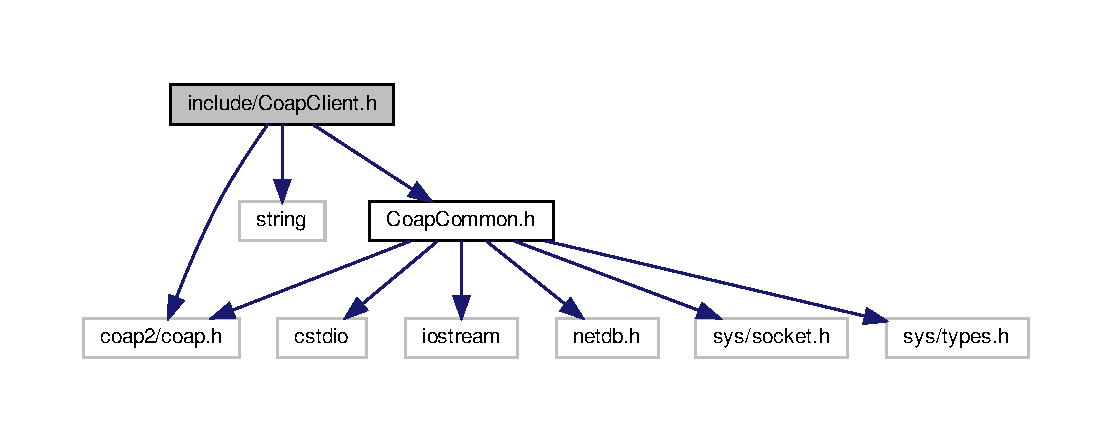
\includegraphics[width=350pt]{CoapClient_8h__incl}
\end{center}
\end{figure}
This graph shows which files directly or indirectly include this file\+:
\nopagebreak
\begin{figure}[H]
\begin{center}
\leavevmode
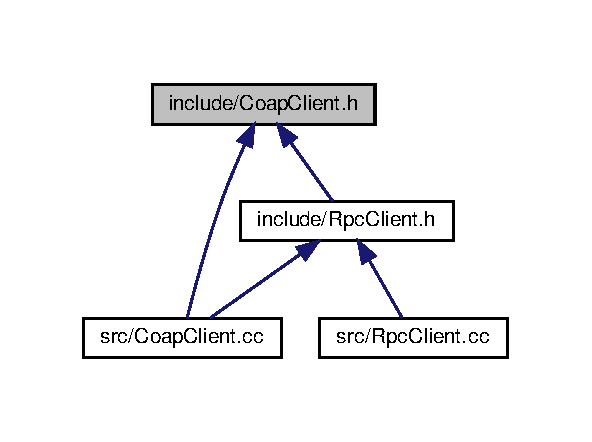
\includegraphics[width=284pt]{CoapClient_8h__dep__incl}
\end{center}
\end{figure}
\subsection*{Classes}
\begin{DoxyCompactItemize}
\item 
struct \hyperlink{structClientParams}{Client\+Params}
\item 
class \hyperlink{classcoappbrpc_1_1CoapClient}{coappbrpc\+::\+Coap\+Client}
\end{DoxyCompactItemize}


\subsection{Detailed Description}
Client Handling for Co\+AP protocol. 


\hypertarget{CoapCommon_8h}{}\section{include/\+Coap\+Common.h File Reference}
\label{CoapCommon_8h}\index{include/\+Coap\+Common.\+h@{include/\+Coap\+Common.\+h}}


Common function to resolve address used by both coap client and coap server.  


{\ttfamily \#include $<$coap2/coap.\+h$>$}\newline
{\ttfamily \#include $<$cstdio$>$}\newline
{\ttfamily \#include $<$iostream$>$}\newline
{\ttfamily \#include $<$netdb.\+h$>$}\newline
{\ttfamily \#include $<$sys/socket.\+h$>$}\newline
{\ttfamily \#include $<$sys/types.\+h$>$}\newline
Include dependency graph for Coap\+Common.\+h\+:\nopagebreak
\begin{figure}[H]
\begin{center}
\leavevmode
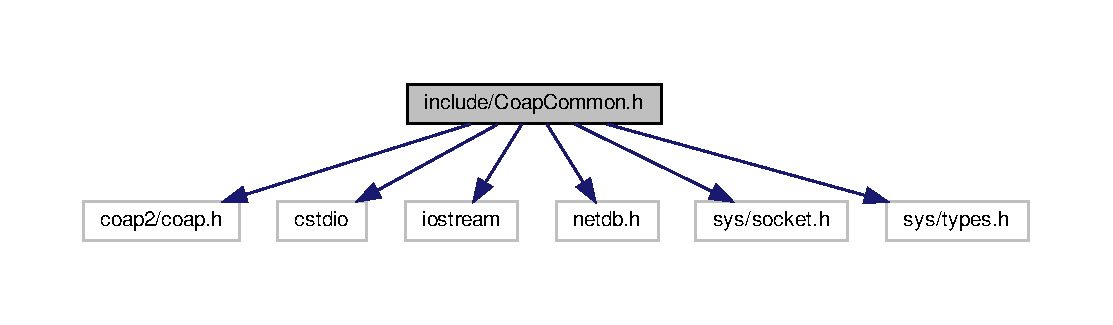
\includegraphics[width=350pt]{CoapCommon_8h__incl}
\end{center}
\end{figure}
This graph shows which files directly or indirectly include this file\+:\nopagebreak
\begin{figure}[H]
\begin{center}
\leavevmode
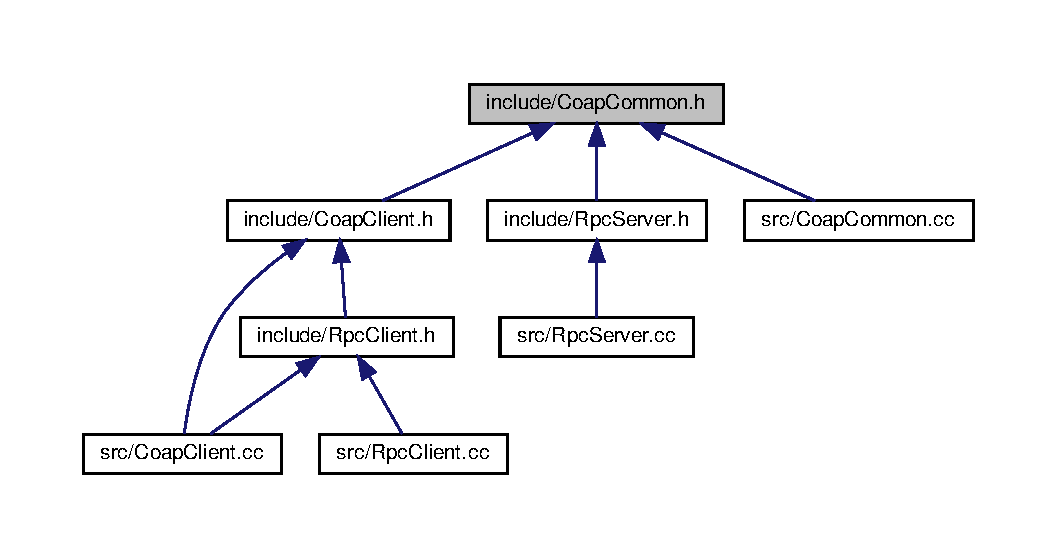
\includegraphics[width=350pt]{CoapCommon_8h__dep__incl}
\end{center}
\end{figure}
\subsection*{Classes}
\begin{DoxyCompactItemize}
\item 
class \hyperlink{classCoapCommon}{Coap\+Common}
\end{DoxyCompactItemize}
\subsection*{Macros}
\begin{DoxyCompactItemize}
\item 
\mbox{\Hypertarget{CoapCommon_8h_a064db62080cf9c526cb56e1b512427e2}\label{CoapCommon_8h_a064db62080cf9c526cb56e1b512427e2}} 
\#define \hyperlink{CoapCommon_8h_a064db62080cf9c526cb56e1b512427e2}{C\+O\+A\+P\+\_\+\+I\+N\+T\+E\+R\+F\+A\+C\+E\+\_\+\+N\+A\+ME}~\char`\"{}rpc\char`\"{}
\begin{DoxyCompactList}\small\item\em A macro containing name of U\+RI to be used in C\+O\+AP request. \end{DoxyCompactList}\end{DoxyCompactItemize}


\subsection{Detailed Description}
Common function to resolve address used by both coap client and coap server. 


\hypertarget{ControllerRPC_8h}{}\section{include/\+Controller\+R\+PC.h File Reference}
\label{ControllerRPC_8h}\index{include/\+Controller\+R\+P\+C.\+h@{include/\+Controller\+R\+P\+C.\+h}}


Controls R\+PC, resets, sets failed if R\+PC failes, handles error messages.  


{\ttfamily \#include \char`\"{}Msg\+Schema.\+pb.\+h\char`\"{}}\newline
{\ttfamily \#include $<$google/protobuf/service.\+h$>$}\newline
{\ttfamily \#include $<$string$>$}\newline
Include dependency graph for Controller\+R\+P\+C.\+h\+:\nopagebreak
\begin{figure}[H]
\begin{center}
\leavevmode
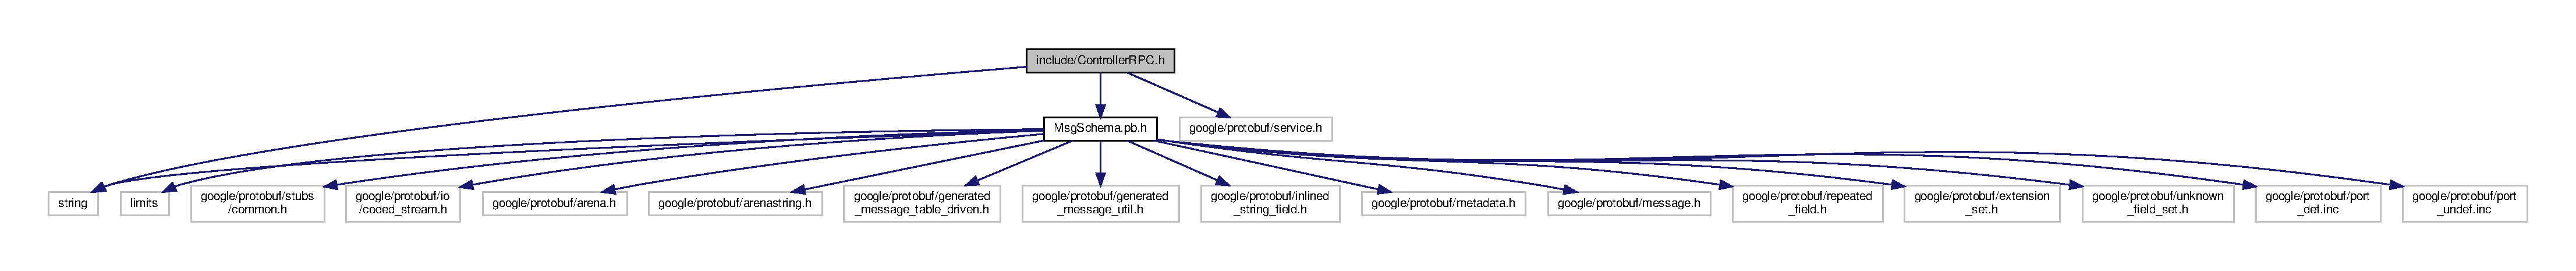
\includegraphics[width=350pt]{ControllerRPC_8h__incl}
\end{center}
\end{figure}
This graph shows which files directly or indirectly include this file\+:\nopagebreak
\begin{figure}[H]
\begin{center}
\leavevmode
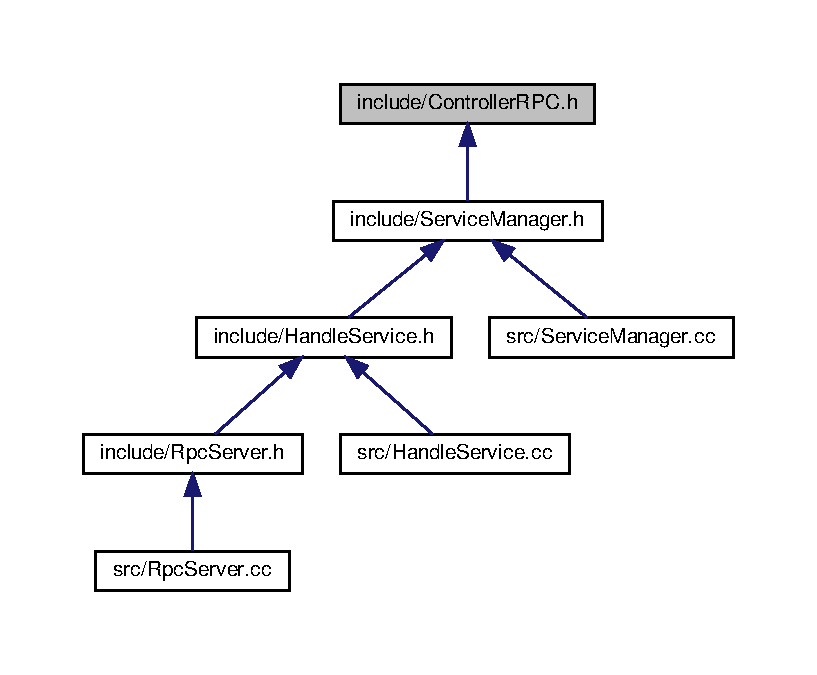
\includegraphics[width=350pt]{ControllerRPC_8h__dep__incl}
\end{center}
\end{figure}
\subsection*{Classes}
\begin{DoxyCompactItemize}
\item 
class \hyperlink{classcoappbrpc_1_1ControllerRPC}{coappbrpc\+::\+Controller\+R\+PC}
\end{DoxyCompactItemize}


\subsection{Detailed Description}
Controls R\+PC, resets, sets failed if R\+PC failes, handles error messages. 


\hypertarget{HandleService_8h}{}\section{include/\+Handle\+Service.h File Reference}
\label{HandleService_8h}\index{include/\+Handle\+Service.\+h@{include/\+Handle\+Service.\+h}}


Handles R\+PC service and registry of services.  


{\ttfamily \#include \char`\"{}Service\+Manager.\+h\char`\"{}}\newline
{\ttfamily \#include $<$google/protobuf/service.\+h$>$}\newline
{\ttfamily \#include $<$string$>$}\newline
Include dependency graph for Handle\+Service.\+h\+:
\nopagebreak
\begin{figure}[H]
\begin{center}
\leavevmode
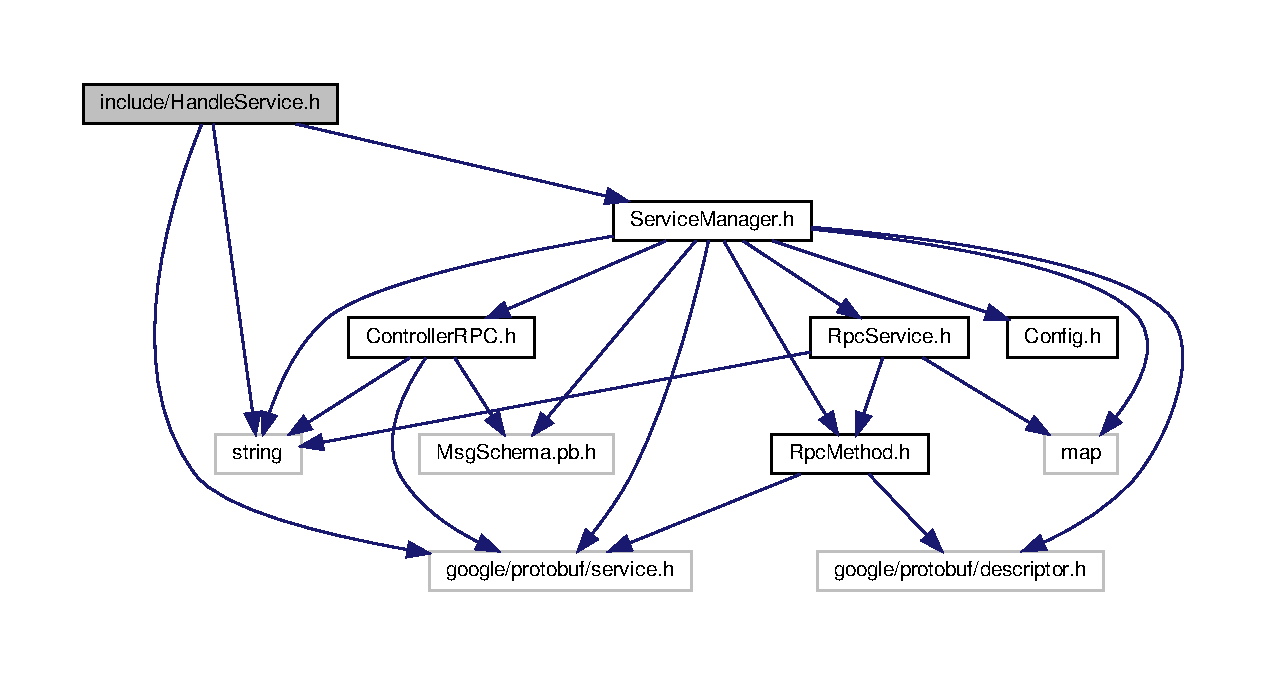
\includegraphics[width=350pt]{HandleService_8h__incl}
\end{center}
\end{figure}
This graph shows which files directly or indirectly include this file\+:
\nopagebreak
\begin{figure}[H]
\begin{center}
\leavevmode
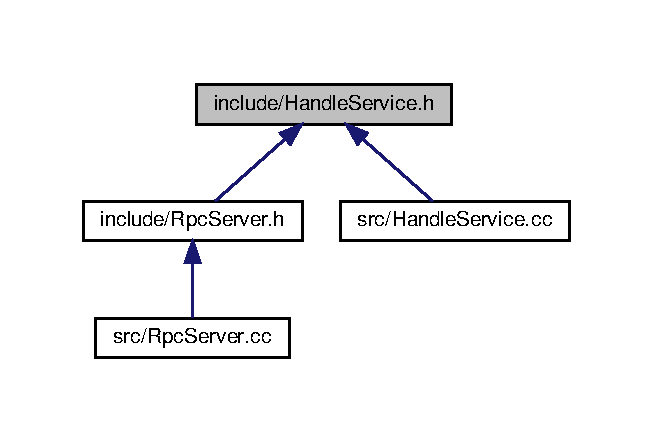
\includegraphics[width=314pt]{HandleService_8h__dep__incl}
\end{center}
\end{figure}
\subsection*{Functions}
\begin{DoxyCompactItemize}
\item 
string \hyperlink{HandleService_8h_a9e514884c719781f5f98d5b81f426177}{coappbrpc\+::handle\+Service} (const char $\ast$, const size\+\_\+t)
\begin{DoxyCompactList}\small\item\em Uses handle\+R\+PC function of \hyperlink{classcoappbrpc_1_1ServiceManager}{Service\+Manager} instance. error. \end{DoxyCompactList}\item 
void \hyperlink{HandleService_8h_ae35f0cbe6fe555f7f59d061063c39b93}{coappbrpc\+::handle\+Reg\+Service} (Service $\ast$)
\begin{DoxyCompactList}\small\item\em Uses register Service function of \hyperlink{classcoappbrpc_1_1ServiceManager}{Service\+Manager} instance. error. \end{DoxyCompactList}\end{DoxyCompactItemize}


\subsection{Detailed Description}
Handles R\+PC service and registry of services. 



\subsection{Function Documentation}
\mbox{\Hypertarget{HandleService_8h_file_ae35f0cbe6fe555f7f59d061063c39b93}\label{HandleService_8h_file_ae35f0cbe6fe555f7f59d061063c39b93}} 
\index{Handle\+Service.\+h@{Handle\+Service.\+h}!handle\+Reg\+Service@{handle\+Reg\+Service}}
\index{handle\+Reg\+Service@{handle\+Reg\+Service}!Handle\+Service.\+h@{Handle\+Service.\+h}}
\subsubsection{\texorpdfstring{handle\+Reg\+Service()}{handleRegService()}}
{\footnotesize\ttfamily void coappbrpc\+::handle\+Reg\+Service (\begin{DoxyParamCaption}\item[{Service $\ast$}]{service }\end{DoxyParamCaption})}



Uses register Service function of Service\+Manager instance. error. 


\begin{DoxyParams}{Parameters}
{\em service} & Service reference to be sent to Service Manager \\
\hline
\end{DoxyParams}
\mbox{\Hypertarget{HandleService_8h_file_a9e514884c719781f5f98d5b81f426177}\label{HandleService_8h_file_a9e514884c719781f5f98d5b81f426177}} 
\index{Handle\+Service.\+h@{Handle\+Service.\+h}!handle\+Service@{handle\+Service}}
\index{handle\+Service@{handle\+Service}!Handle\+Service.\+h@{Handle\+Service.\+h}}
\subsubsection{\texorpdfstring{handle\+Service()}{handleService()}}
{\footnotesize\ttfamily string coappbrpc\+::handle\+Service (\begin{DoxyParamCaption}\item[{const char $\ast$}]{data,  }\item[{const size\+\_\+t}]{len }\end{DoxyParamCaption})}



Uses handle\+R\+PC function of Service\+Manager instance. error. 


\begin{DoxyParams}{Parameters}
{\em data} & Data reference to be sent to Service Manager, of type char \\
\hline
{\em len} & length of data of type size\+\_\+t \\
\hline
\end{DoxyParams}

\hypertarget{RpcClient_8h}{}\section{include/\+Rpc\+Client.h File Reference}
\label{RpcClient_8h}\index{include/\+Rpc\+Client.\+h@{include/\+Rpc\+Client.\+h}}


Sets Client parameters to be passed as Coap Parameters and calls for execution of Co\+AP protocol.  


{\ttfamily \#include \char`\"{}Coap\+Client.\+h\char`\"{}}\newline
{\ttfamily \#include \char`\"{}Msg\+Schema.\+pb.\+h\char`\"{}}\newline
{\ttfamily \#include $<$iostream$>$}\newline
{\ttfamily \#include $<$string$>$}\newline
Include dependency graph for Rpc\+Client.\+h\+:\nopagebreak
\begin{figure}[H]
\begin{center}
\leavevmode
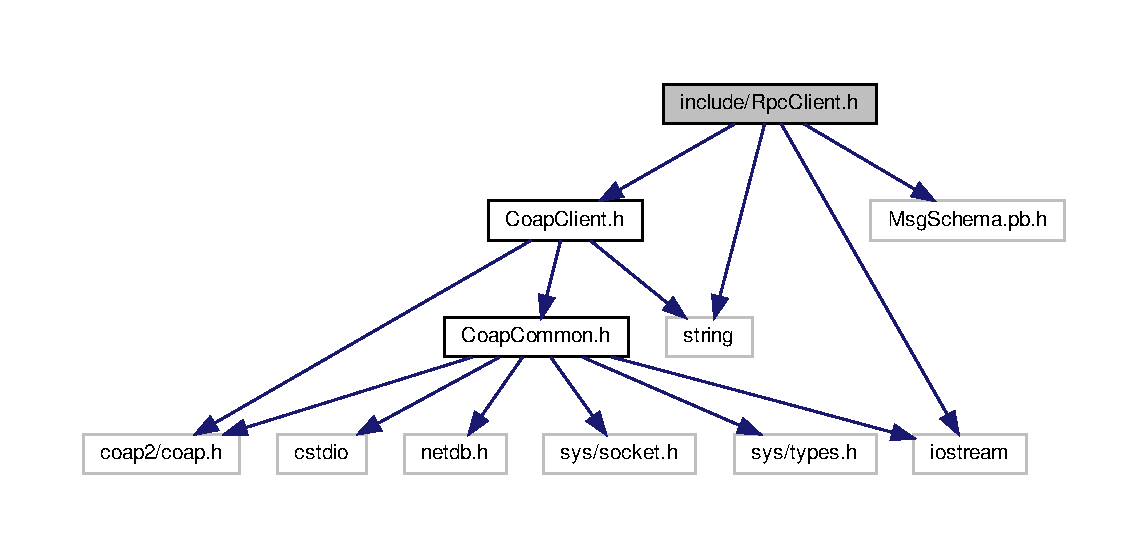
\includegraphics[width=350pt]{RpcClient_8h__incl}
\end{center}
\end{figure}
This graph shows which files directly or indirectly include this file\+:\nopagebreak
\begin{figure}[H]
\begin{center}
\leavevmode
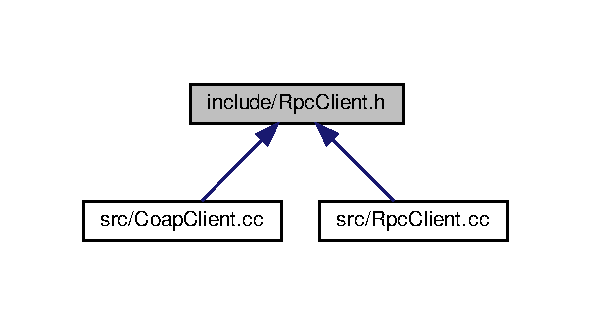
\includegraphics[width=284pt]{RpcClient_8h__dep__incl}
\end{center}
\end{figure}
\subsection*{Classes}
\begin{DoxyCompactItemize}
\item 
class \hyperlink{classcoappbrpc_1_1RpcClient}{coappbrpc\+::\+Rpc\+Client}
\begin{DoxyCompactList}\small\item\em This class contains methods to run client, set responses, get responses, setup server addresses and execute function which is called from client stubs. \end{DoxyCompactList}\end{DoxyCompactItemize}


\subsection{Detailed Description}
Sets Client parameters to be passed as Coap Parameters and calls for execution of Co\+AP protocol. 


\hypertarget{RpcMethod_8h}{}\section{include/\+Rpc\+Method.h File Reference}
\label{RpcMethod_8h}\index{include/\+Rpc\+Method.\+h@{include/\+Rpc\+Method.\+h}}


Handles R\+PC service and registry of services.  


{\ttfamily \#include $<$google/protobuf/descriptor.\+h$>$}\newline
{\ttfamily \#include $<$google/protobuf/service.\+h$>$}\newline
Include dependency graph for Rpc\+Method.\+h\+:
\nopagebreak
\begin{figure}[H]
\begin{center}
\leavevmode
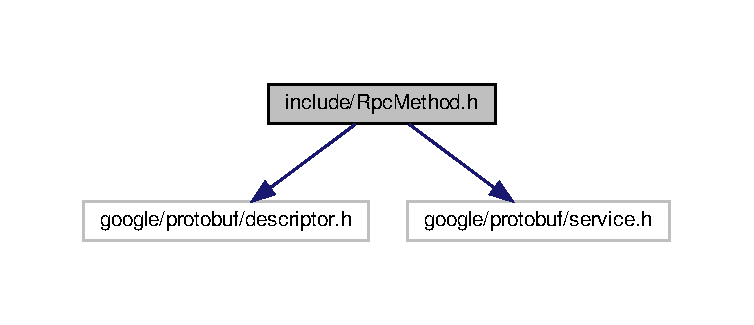
\includegraphics[width=350pt]{RpcMethod_8h__incl}
\end{center}
\end{figure}
This graph shows which files directly or indirectly include this file\+:
\nopagebreak
\begin{figure}[H]
\begin{center}
\leavevmode
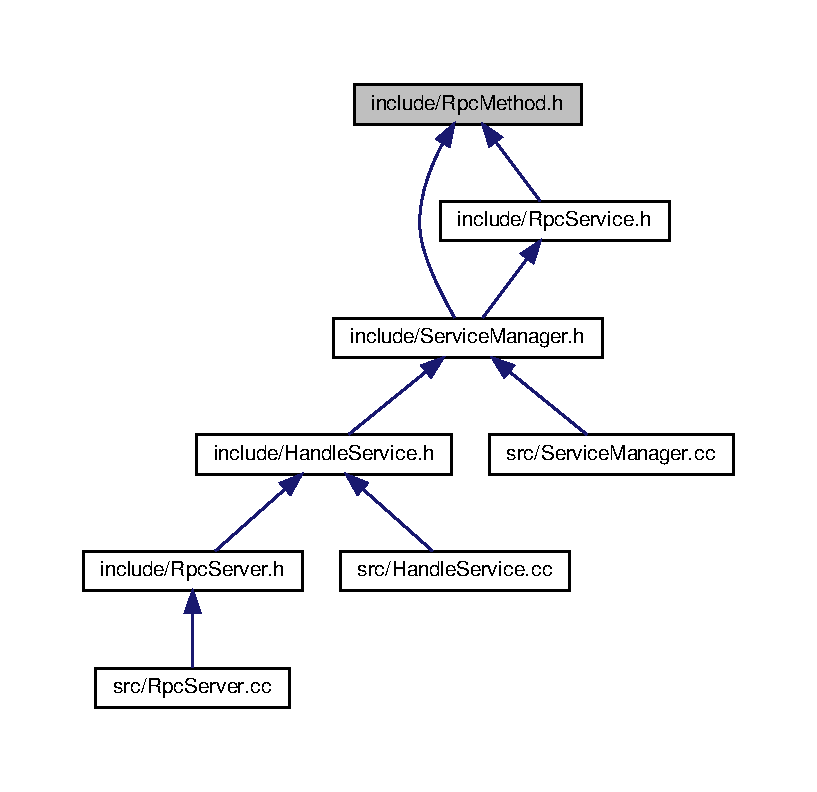
\includegraphics[width=350pt]{RpcMethod_8h__dep__incl}
\end{center}
\end{figure}
\subsection*{Classes}
\begin{DoxyCompactItemize}
\item 
class \hyperlink{classcoappbrpc_1_1RpcMethod}{coappbrpc\+::\+Rpc\+Method}
\end{DoxyCompactItemize}


\subsection{Detailed Description}
Handles R\+PC service and registry of services. 


\hypertarget{RpcServer_8h}{}\section{include/\+Rpc\+Server.h File Reference}
\label{RpcServer_8h}\index{include/\+Rpc\+Server.\+h@{include/\+Rpc\+Server.\+h}}


Server Handling for Co\+AP protocol.  


{\ttfamily \#include \char`\"{}Msg\+Schema.\+pb.\+h\char`\"{}}\newline
{\ttfamily \#include $<$coap2/coap.\+h$>$}\newline
{\ttfamily \#include $<$google/protobuf/service.\+h$>$}\newline
{\ttfamily \#include $<$iostream$>$}\newline
{\ttfamily \#include $<$stdlib.\+h$>$}\newline
{\ttfamily \#include $<$string$>$}\newline
{\ttfamily \#include \char`\"{}Coap\+Common.\+h\char`\"{}}\newline
{\ttfamily \#include \char`\"{}Handle\+Service.\+h\char`\"{}}\newline
Include dependency graph for Rpc\+Server.\+h\+:\nopagebreak
\begin{figure}[H]
\begin{center}
\leavevmode
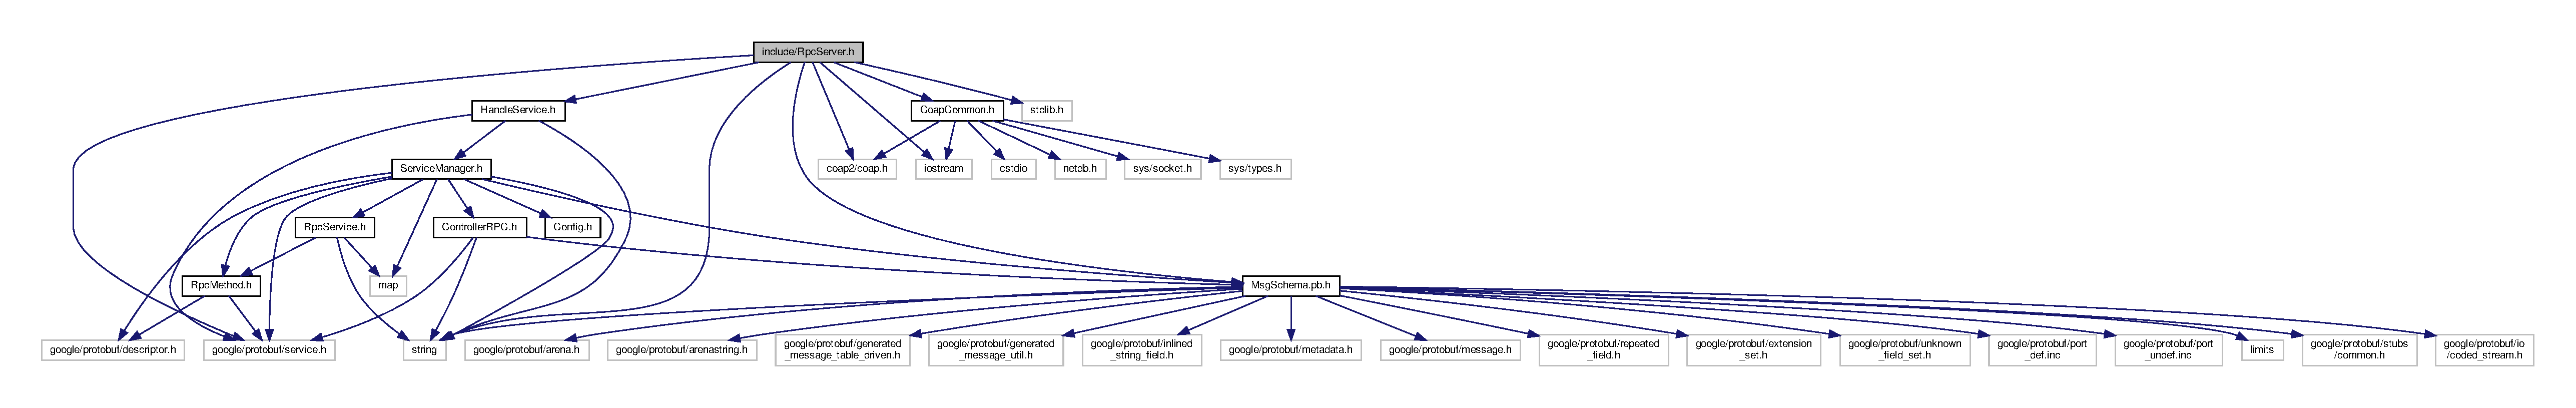
\includegraphics[width=350pt]{RpcServer_8h__incl}
\end{center}
\end{figure}
This graph shows which files directly or indirectly include this file\+:\nopagebreak
\begin{figure}[H]
\begin{center}
\leavevmode
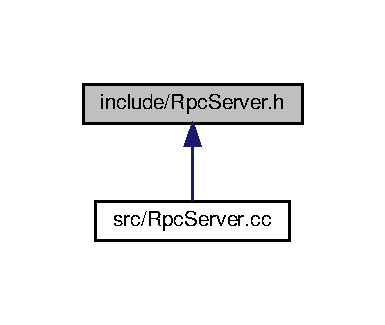
\includegraphics[width=185pt]{RpcServer_8h__dep__incl}
\end{center}
\end{figure}
\subsection*{Classes}
\begin{DoxyCompactItemize}
\item 
class \hyperlink{classcoappbrpc_1_1RpcServer}{coappbrpc\+::\+Rpc\+Server}
\end{DoxyCompactItemize}


\subsection{Detailed Description}
Server Handling for Co\+AP protocol. 


\hypertarget{RpcService_8h}{}\section{include/\+Rpc\+Service.h File Reference}
\label{RpcService_8h}\index{include/\+Rpc\+Service.\+h@{include/\+Rpc\+Service.\+h}}


R\+PC Services Handling , adding methods, getting methods and checking if method exists or not.  


{\ttfamily \#include $<$map$>$}\newline
{\ttfamily \#include $<$string$>$}\newline
{\ttfamily \#include \char`\"{}Rpc\+Method.\+h\char`\"{}}\newline
Include dependency graph for Rpc\+Service.\+h\+:\nopagebreak
\begin{figure}[H]
\begin{center}
\leavevmode
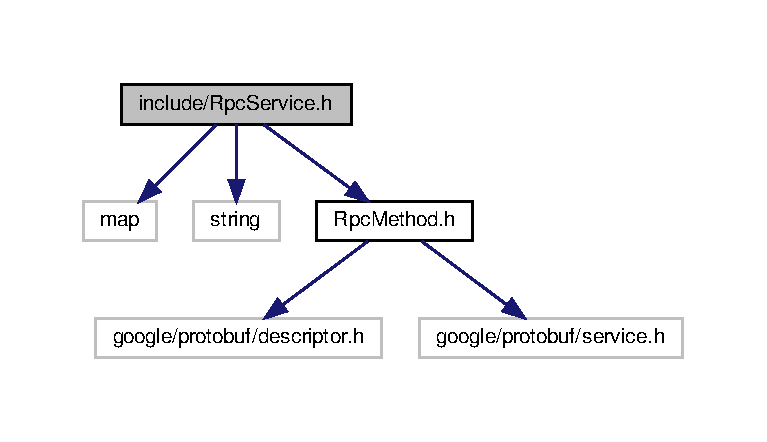
\includegraphics[width=350pt]{RpcService_8h__incl}
\end{center}
\end{figure}
This graph shows which files directly or indirectly include this file\+:\nopagebreak
\begin{figure}[H]
\begin{center}
\leavevmode
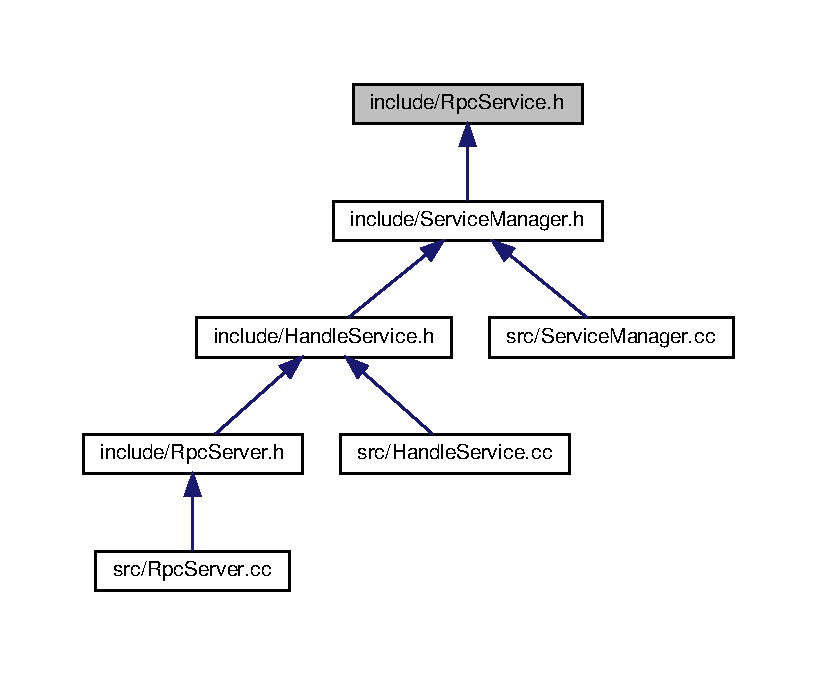
\includegraphics[width=350pt]{RpcService_8h__dep__incl}
\end{center}
\end{figure}
\subsection*{Classes}
\begin{DoxyCompactItemize}
\item 
class \hyperlink{classcoappbrpc_1_1RpcService}{coappbrpc\+::\+Rpc\+Service}
\begin{DoxyCompactList}\small\item\em This class defines service for remote calls. It has methods for adding rpc methods, getting methods, validating if method exists. \end{DoxyCompactList}\end{DoxyCompactItemize}


\subsection{Detailed Description}
R\+PC Services Handling , adding methods, getting methods and checking if method exists or not. 


\hypertarget{ServiceManager_8h}{}\section{include/\+Service\+Manager.h File Reference}
\label{ServiceManager_8h}\index{include/\+Service\+Manager.\+h@{include/\+Service\+Manager.\+h}}


Handles Service creation, registration, getting and setting Services, handles R\+PC and validates requests.  


{\ttfamily \#include $<$map$>$}\newline
{\ttfamily \#include $<$string$>$}\newline
{\ttfamily \#include $<$google/protobuf/descriptor.\+h$>$}\newline
{\ttfamily \#include $<$google/protobuf/service.\+h$>$}\newline
{\ttfamily \#include \char`\"{}Config.\+h\char`\"{}}\newline
{\ttfamily \#include \char`\"{}Controller\+R\+P\+C.\+h\char`\"{}}\newline
{\ttfamily \#include \char`\"{}Rpc\+Method.\+h\char`\"{}}\newline
{\ttfamily \#include \char`\"{}Rpc\+Service.\+h\char`\"{}}\newline
{\ttfamily \#include \char`\"{}Msg\+Schema.\+pb.\+h\char`\"{}}\newline
Include dependency graph for Service\+Manager.\+h\+:\nopagebreak
\begin{figure}[H]
\begin{center}
\leavevmode
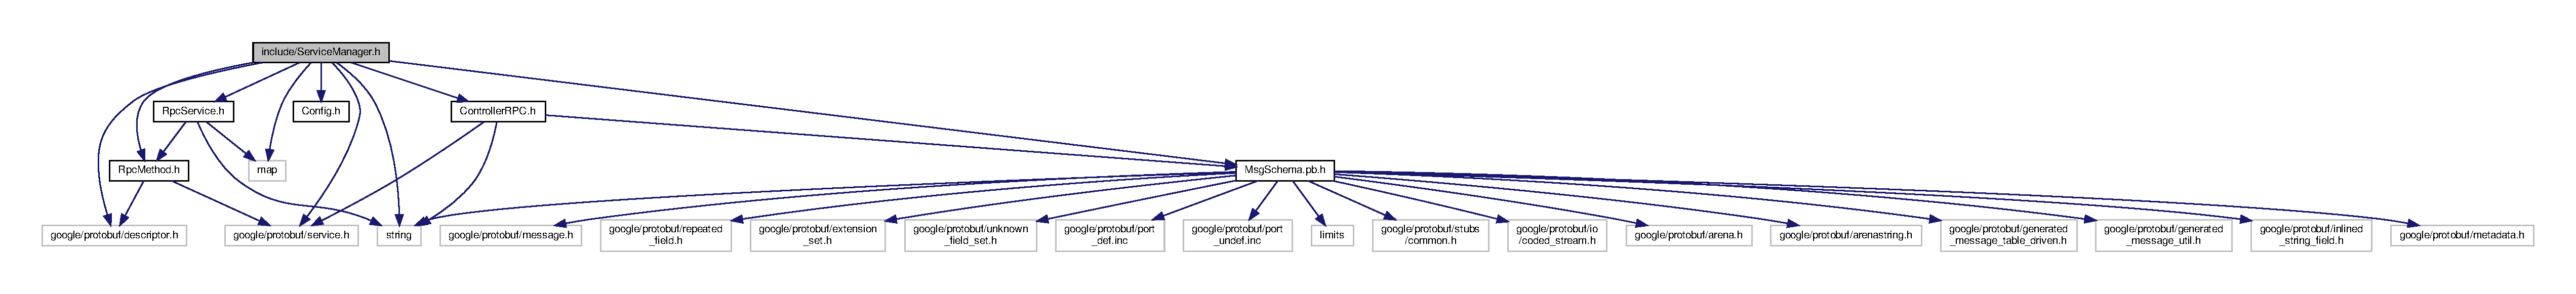
\includegraphics[width=350pt]{ServiceManager_8h__incl}
\end{center}
\end{figure}
This graph shows which files directly or indirectly include this file\+:\nopagebreak
\begin{figure}[H]
\begin{center}
\leavevmode
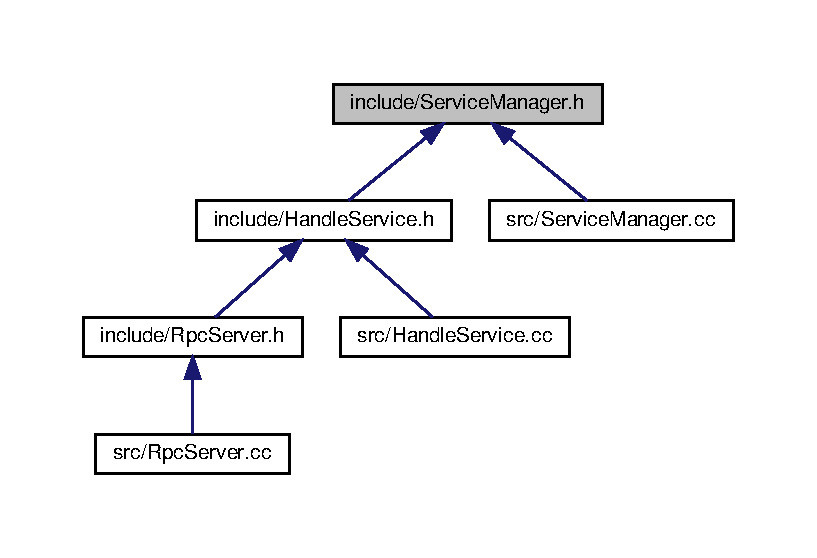
\includegraphics[width=350pt]{ServiceManager_8h__dep__incl}
\end{center}
\end{figure}
\subsection*{Classes}
\begin{DoxyCompactItemize}
\item 
class \hyperlink{classcoappbrpc_1_1ServiceManager}{coappbrpc\+::\+Service\+Manager}
\begin{DoxyCompactList}\small\item\em This class contains methods to handle R\+PC, register services, get services, get method details, validate passed parameters, validate requests, validate versions, and check if services are already existed or not. \end{DoxyCompactList}\end{DoxyCompactItemize}


\subsection{Detailed Description}
Handles Service creation, registration, getting and setting Services, handles R\+PC and validates requests. 


\hypertarget{CoapClient_8cc}{}\section{src/\+Coap\+Client.cc File Reference}
\label{CoapClient_8cc}\index{src/\+Coap\+Client.\+cc@{src/\+Coap\+Client.\+cc}}


Client Handling for Co\+AP protocol.  


{\ttfamily \#include \char`\"{}Coap\+Client.\+h\char`\"{}}\newline
{\ttfamily \#include \char`\"{}Rpc\+Client.\+h\char`\"{}}\newline
Include dependency graph for Coap\+Client.\+cc\+:\nopagebreak
\begin{figure}[H]
\begin{center}
\leavevmode
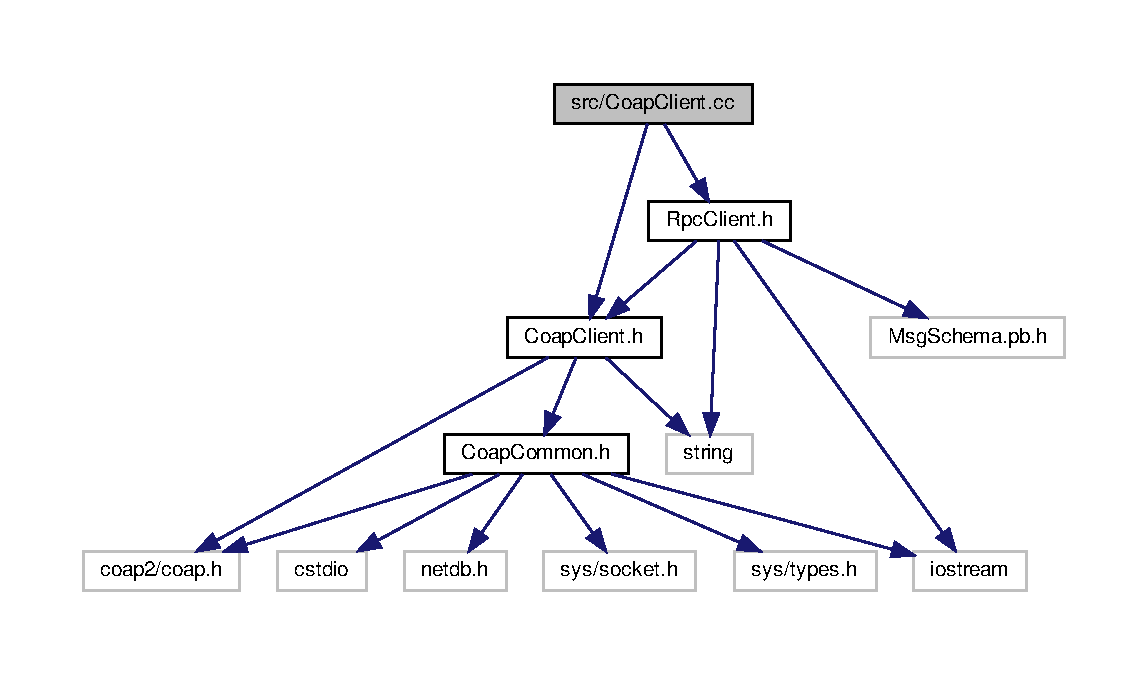
\includegraphics[width=350pt]{CoapClient_8cc__incl}
\end{center}
\end{figure}


\subsection{Detailed Description}
Client Handling for Co\+AP protocol. 


\hypertarget{CoapCommon_8cc}{}\section{src/\+Coap\+Common.cc File Reference}
\label{CoapCommon_8cc}\index{src/\+Coap\+Common.\+cc@{src/\+Coap\+Common.\+cc}}


Common function to resolve address used by both coap client and coap server.  


{\ttfamily \#include \char`\"{}Coap\+Common.\+h\char`\"{}}\newline
Include dependency graph for Coap\+Common.\+cc\+:
\nopagebreak
\begin{figure}[H]
\begin{center}
\leavevmode
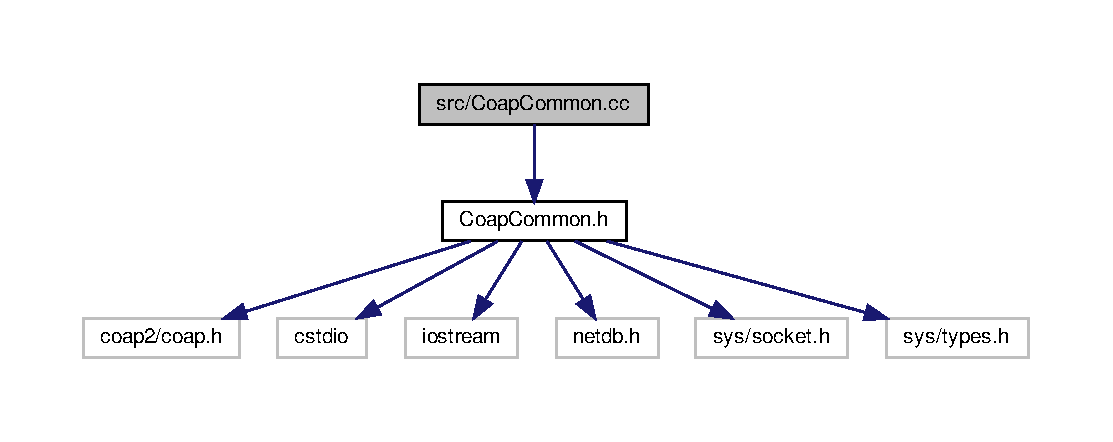
\includegraphics[width=350pt]{CoapCommon_8cc__incl}
\end{center}
\end{figure}


\subsection{Detailed Description}
Common function to resolve address used by both coap client and coap server. 


\hypertarget{HandleService_8cc}{}\section{src/\+Handle\+Service.cc File Reference}
\label{HandleService_8cc}\index{src/\+Handle\+Service.\+cc@{src/\+Handle\+Service.\+cc}}


Handles R\+PC service and registry of services.  


{\ttfamily \#include \char`\"{}Handle\+Service.\+h\char`\"{}}\newline
Include dependency graph for Handle\+Service.\+cc\+:
\nopagebreak
\begin{figure}[H]
\begin{center}
\leavevmode
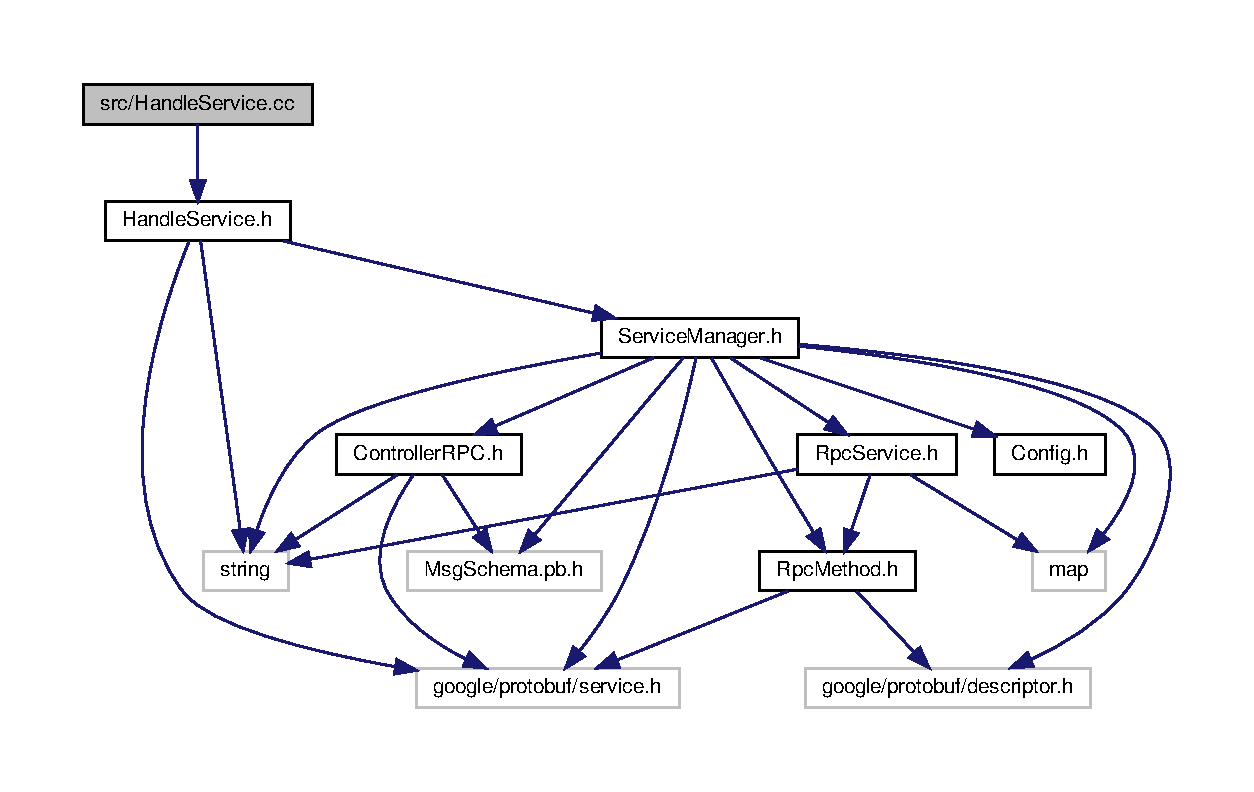
\includegraphics[width=350pt]{HandleService_8cc__incl}
\end{center}
\end{figure}
\subsection*{Functions}
\begin{DoxyCompactItemize}
\item 
string \hyperlink{HandleService_8h_a9e514884c719781f5f98d5b81f426177}{coappbrpc\+::handle\+Service} (const char $\ast$, const size\+\_\+t)
\begin{DoxyCompactList}\small\item\em Uses handle\+R\+PC function of \hyperlink{classcoappbrpc_1_1ServiceManager}{Service\+Manager} instance. error. \end{DoxyCompactList}\item 
void \hyperlink{HandleService_8h_ae35f0cbe6fe555f7f59d061063c39b93}{coappbrpc\+::handle\+Reg\+Service} (Service $\ast$)
\begin{DoxyCompactList}\small\item\em Uses register Service function of \hyperlink{classcoappbrpc_1_1ServiceManager}{Service\+Manager} instance. error. \end{DoxyCompactList}\end{DoxyCompactItemize}
\subsection*{Variables}
\begin{DoxyCompactItemize}
\item 
\mbox{\Hypertarget{HandleService_8cc_a4358e4719668d75dbda322877e3c1409}\label{HandleService_8cc_a4358e4719668d75dbda322877e3c1409}} 
Service\+Manager {\bfseries coappbrpc\+::\+\_\+\+\_\+srv\+\_\+man}
\end{DoxyCompactItemize}


\subsection{Detailed Description}
Handles R\+PC service and registry of services. 



\subsection{Function Documentation}
\mbox{\Hypertarget{HandleService_8h_file_ae35f0cbe6fe555f7f59d061063c39b93}\label{HandleService_8h_file_ae35f0cbe6fe555f7f59d061063c39b93}} 
\index{Handle\+Service.\+cc@{Handle\+Service.\+cc}!handle\+Reg\+Service@{handle\+Reg\+Service}}
\index{handle\+Reg\+Service@{handle\+Reg\+Service}!Handle\+Service.\+cc@{Handle\+Service.\+cc}}
\subsubsection{\texorpdfstring{handle\+Reg\+Service()}{handleRegService()}}
{\footnotesize\ttfamily void coappbrpc\+::handle\+Reg\+Service (\begin{DoxyParamCaption}\item[{Service $\ast$}]{service }\end{DoxyParamCaption})}



Uses register Service function of Service\+Manager instance. error. 


\begin{DoxyParams}{Parameters}
{\em service} & Service reference to be sent to Service Manager \\
\hline
\end{DoxyParams}
\mbox{\Hypertarget{HandleService_8h_file_a9e514884c719781f5f98d5b81f426177}\label{HandleService_8h_file_a9e514884c719781f5f98d5b81f426177}} 
\index{Handle\+Service.\+cc@{Handle\+Service.\+cc}!handle\+Service@{handle\+Service}}
\index{handle\+Service@{handle\+Service}!Handle\+Service.\+cc@{Handle\+Service.\+cc}}
\subsubsection{\texorpdfstring{handle\+Service()}{handleService()}}
{\footnotesize\ttfamily string coappbrpc\+::handle\+Service (\begin{DoxyParamCaption}\item[{const char $\ast$}]{data,  }\item[{const size\+\_\+t}]{len }\end{DoxyParamCaption})}



Uses handle\+R\+PC function of Service\+Manager instance. error. 


\begin{DoxyParams}{Parameters}
{\em data} & Data reference to be sent to Service Manager, of type char \\
\hline
{\em len} & length of data of type size\+\_\+t \\
\hline
\end{DoxyParams}

\hypertarget{RpcClient_8cc}{}\section{src/\+Rpc\+Client.cc File Reference}
\label{RpcClient_8cc}\index{src/\+Rpc\+Client.\+cc@{src/\+Rpc\+Client.\+cc}}


Sets Client parameters to be passed as Coap Parameters and calls for execution of Co\+AP protocol.  


{\ttfamily \#include \char`\"{}Rpc\+Client.\+h\char`\"{}}\newline
Include dependency graph for Rpc\+Client.\+cc\+:\nopagebreak
\begin{figure}[H]
\begin{center}
\leavevmode
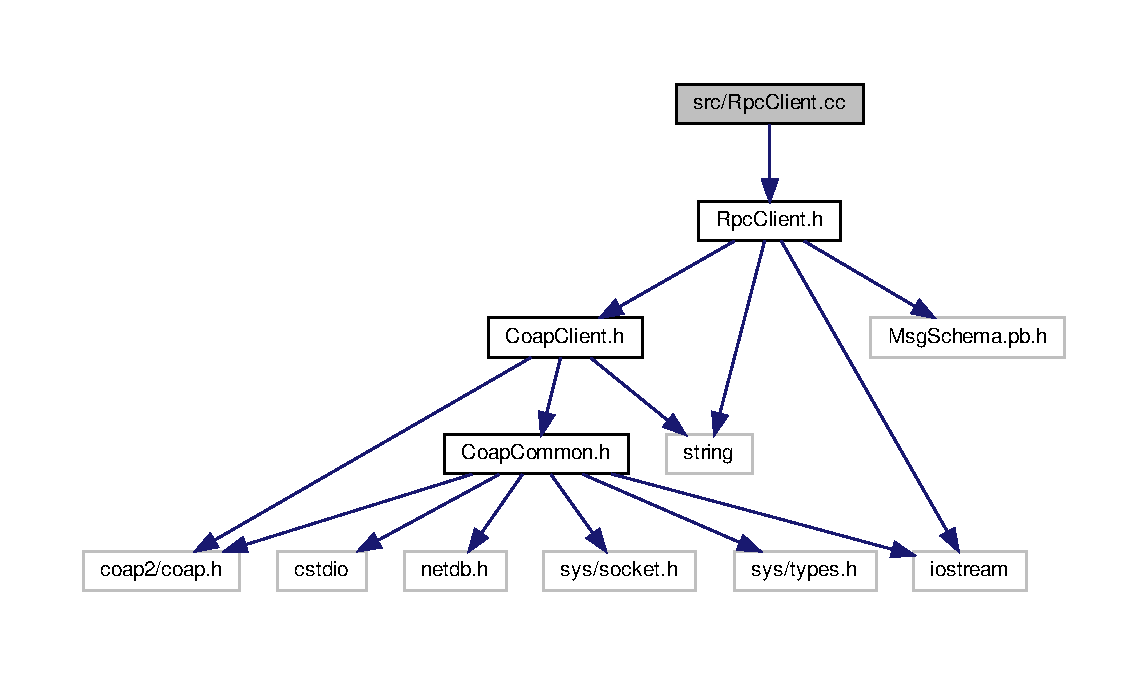
\includegraphics[width=350pt]{RpcClient_8cc__incl}
\end{center}
\end{figure}


\subsection{Detailed Description}
Sets Client parameters to be passed as Coap Parameters and calls for execution of Co\+AP protocol. 


\hypertarget{RpcServer_8cc}{}\section{src/\+Rpc\+Server.cc File Reference}
\label{RpcServer_8cc}\index{src/\+Rpc\+Server.\+cc@{src/\+Rpc\+Server.\+cc}}


Server Handling for Co\+AP protocol.  


{\ttfamily \#include \char`\"{}Rpc\+Server.\+h\char`\"{}}\newline
Include dependency graph for Rpc\+Server.\+cc\+:\nopagebreak
\begin{figure}[H]
\begin{center}
\leavevmode
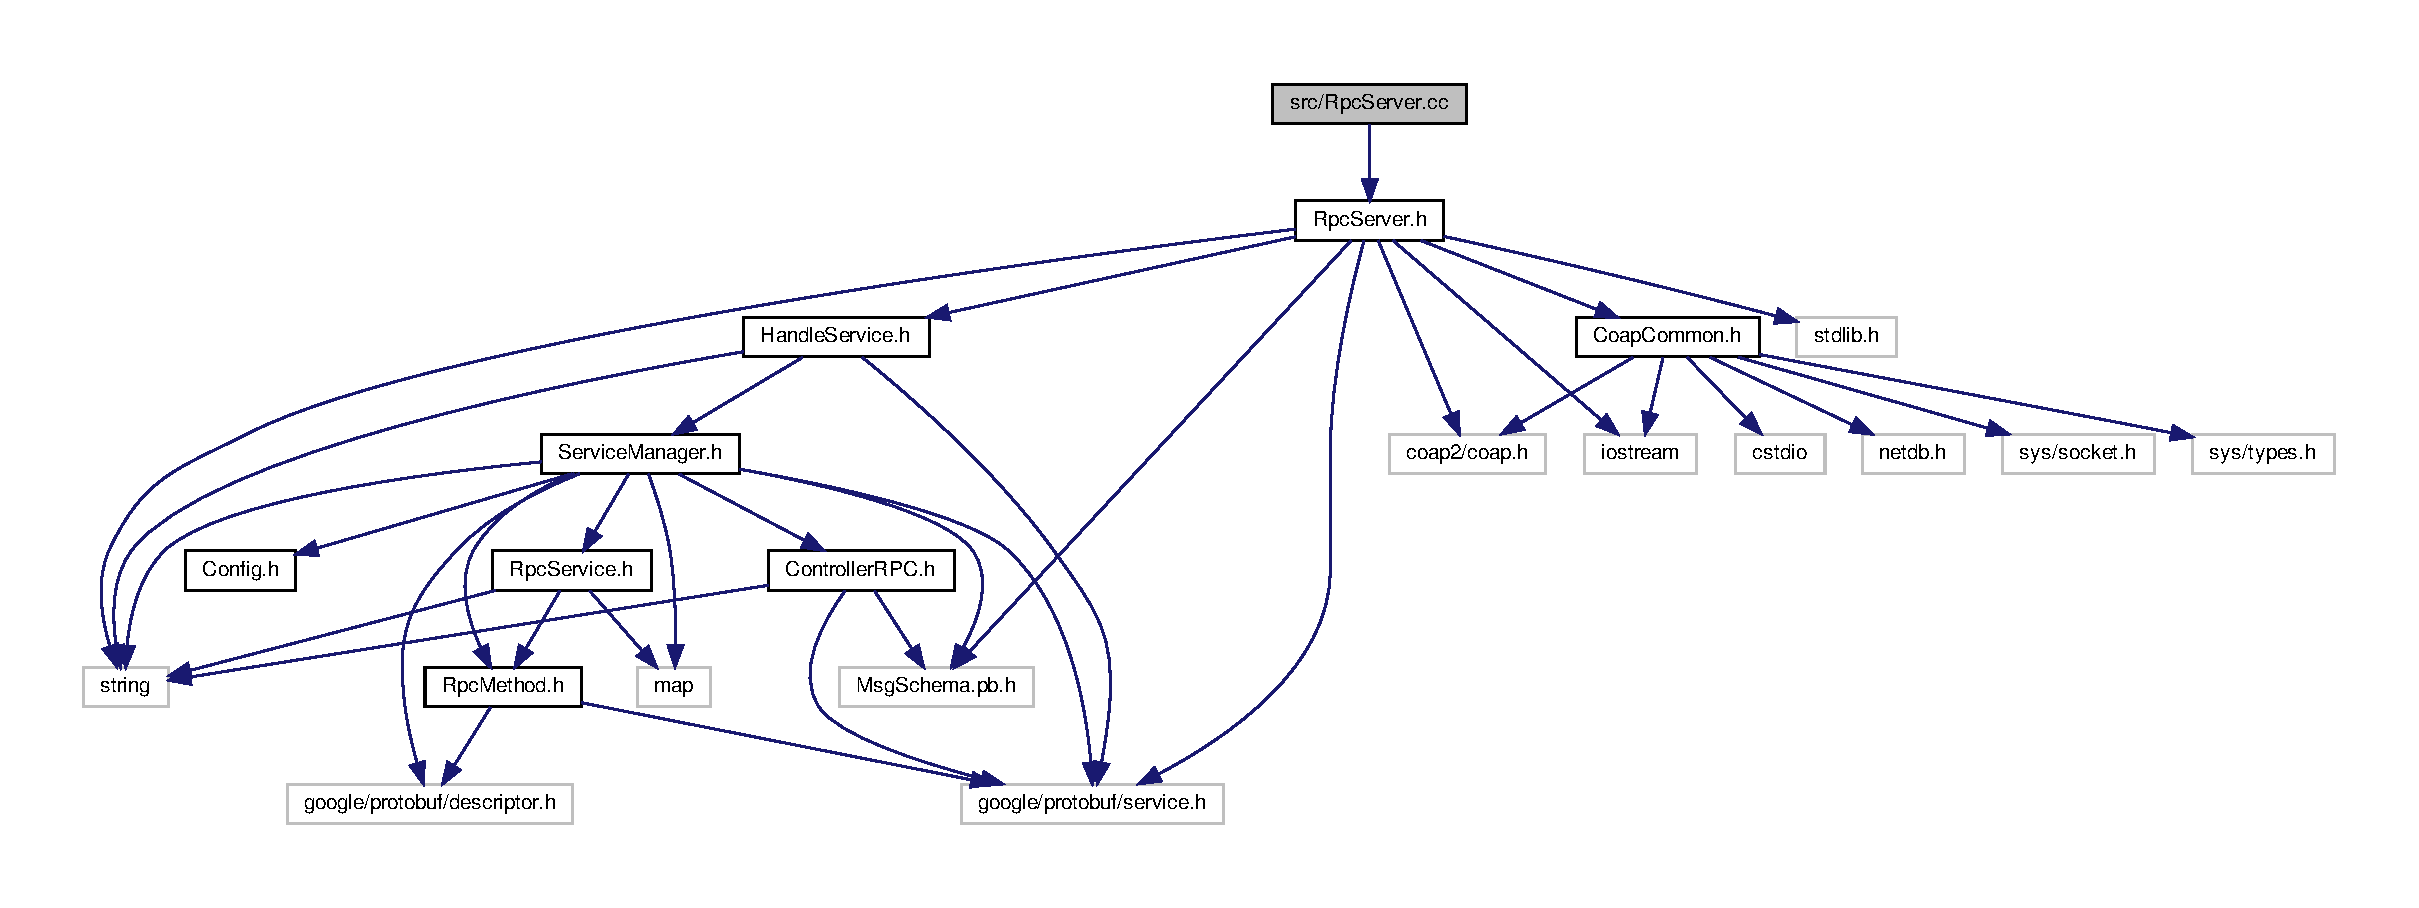
\includegraphics[width=350pt]{RpcServer_8cc__incl}
\end{center}
\end{figure}
\subsection*{Functions}
\begin{DoxyCompactItemize}
\item 
void \hyperlink{RpcServer_8cc_a9e01846fbd4bcab8aacc8f22e7dfb61b}{coappbrpc\+::return\+\_\+handler} (coap\+\_\+context\+\_\+t $\ast$ctx, struct coap\+\_\+resource\+\_\+t $\ast$resource, coap\+\_\+session\+\_\+t $\ast$session, coap\+\_\+pdu\+\_\+t $\ast$request, coap\+\_\+binary\+\_\+t $\ast$token, coap\+\_\+string\+\_\+t $\ast$query, coap\+\_\+pdu\+\_\+t $\ast$response)
\begin{DoxyCompactList}\small\item\em Callback function that sets response data to be sent back to R\+PC client. \end{DoxyCompactList}\end{DoxyCompactItemize}


\subsection{Detailed Description}
Server Handling for Co\+AP protocol. 



\subsection{Function Documentation}
\mbox{\Hypertarget{RpcServer_8cc_file_a9e01846fbd4bcab8aacc8f22e7dfb61b}\label{RpcServer_8cc_file_a9e01846fbd4bcab8aacc8f22e7dfb61b}} 
\index{Rpc\+Server.\+cc@{Rpc\+Server.\+cc}!return\+\_\+handler@{return\+\_\+handler}}
\index{return\+\_\+handler@{return\+\_\+handler}!Rpc\+Server.\+cc@{Rpc\+Server.\+cc}}
\subsubsection{\texorpdfstring{return\+\_\+handler()}{return\_handler()}}
{\footnotesize\ttfamily void coappbrpc\+::return\+\_\+handler (\begin{DoxyParamCaption}\item[{coap\+\_\+context\+\_\+t $\ast$}]{ctx,  }\item[{struct coap\+\_\+resource\+\_\+t $\ast$}]{resource,  }\item[{coap\+\_\+session\+\_\+t $\ast$}]{session,  }\item[{coap\+\_\+pdu\+\_\+t $\ast$}]{request,  }\item[{coap\+\_\+binary\+\_\+t $\ast$}]{token,  }\item[{coap\+\_\+string\+\_\+t $\ast$}]{query,  }\item[{coap\+\_\+pdu\+\_\+t $\ast$}]{response }\end{DoxyParamCaption})}



Callback function that sets response data to be sent back to R\+PC client. 


\begin{DoxyParams}{Parameters}
{\em ctx} & Coap context variable reference of type struct coap\+\_\+context\+\_\+t. \\
\hline
{\em resource} & Coap resource referece. \\
\hline
{\em session} & Coap Session variable reference of type coap\+\_\+session\+\_\+t \\
\hline
{\em request} & Co\+AP P\+DU request received by server \\
\hline
{\em token} & Co\+AP unique token references \\
\hline
{\em query} & Co\+AP query reference \\
\hline
{\em response} & Co\+AP P\+DU response reference for storing data to be returned from Server \\
\hline
\end{DoxyParams}

\hypertarget{ServiceManager_8cc}{}\section{src/\+Service\+Manager.cc File Reference}
\label{ServiceManager_8cc}\index{src/\+Service\+Manager.\+cc@{src/\+Service\+Manager.\+cc}}


Handles Service creation, registration, getting and setting Services, handles R\+PC and validates requests.  


{\ttfamily \#include \char`\"{}Service\+Manager.\+h\char`\"{}}\newline
Include dependency graph for Service\+Manager.\+cc\+:
\nopagebreak
\begin{figure}[H]
\begin{center}
\leavevmode
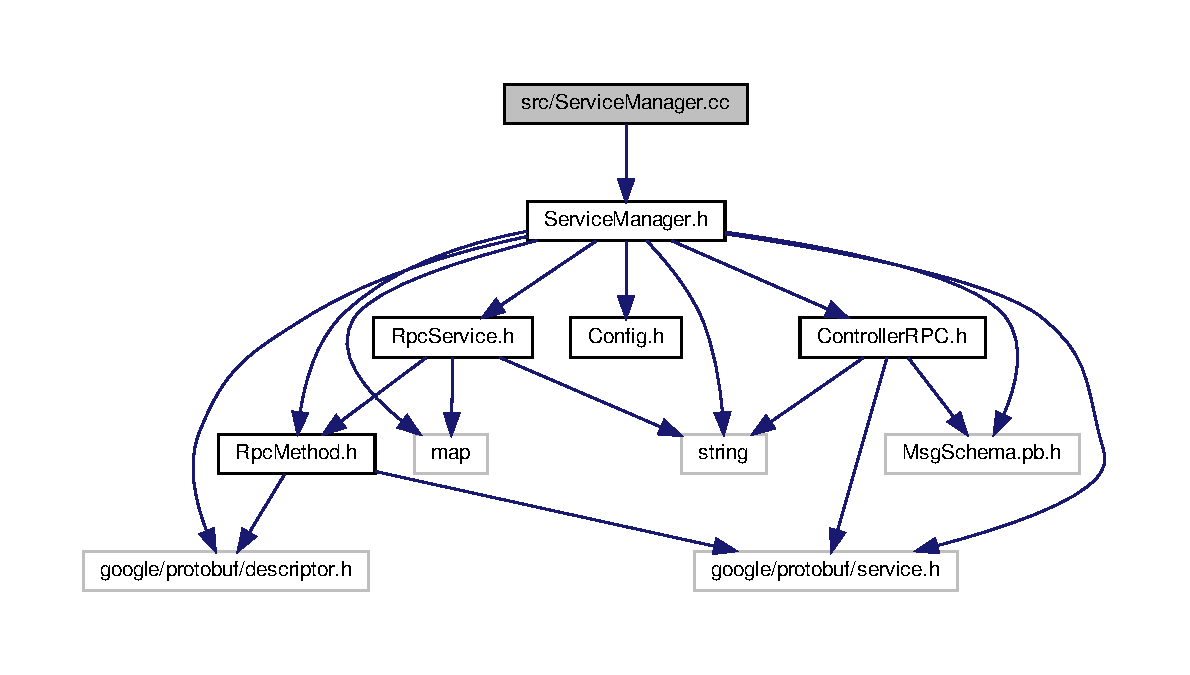
\includegraphics[width=350pt]{ServiceManager_8cc__incl}
\end{center}
\end{figure}
\subsection*{Functions}
\begin{DoxyCompactItemize}
\item 
\mbox{\Hypertarget{ServiceManager_8cc_a301fc8b0fb4b4295f18931bc93ac5fc4}\label{ServiceManager_8cc_a301fc8b0fb4b4295f18931bc93ac5fc4}} 
void {\bfseries coappbrpc\+::gen\+Response} (string \&ret, Response \&rpc\+Response, Message $\ast$response, Controller\+R\+PC $\ast$controller)
\end{DoxyCompactItemize}


\subsection{Detailed Description}
Handles Service creation, registration, getting and setting Services, handles R\+PC and validates requests. 


%--- End generated contents ---

% Index
\backmatter
\newpage
\phantomsection
\clearemptydoublepage
\addcontentsline{toc}{chapter}{Index}
\printindex

\end{document}
